% Options for packages loaded elsewhere
\PassOptionsToPackage{unicode}{hyperref}
\PassOptionsToPackage{hyphens}{url}
%
\documentclass[
]{book}
\usepackage{amsmath,amssymb}
\usepackage{lmodern}
\usepackage{iftex}
\ifPDFTeX
  \usepackage[T1]{fontenc}
  \usepackage[utf8]{inputenc}
  \usepackage{textcomp} % provide euro and other symbols
\else % if luatex or xetex
  \usepackage{unicode-math}
  \defaultfontfeatures{Scale=MatchLowercase}
  \defaultfontfeatures[\rmfamily]{Ligatures=TeX,Scale=1}
\fi
% Use upquote if available, for straight quotes in verbatim environments
\IfFileExists{upquote.sty}{\usepackage{upquote}}{}
\IfFileExists{microtype.sty}{% use microtype if available
  \usepackage[]{microtype}
  \UseMicrotypeSet[protrusion]{basicmath} % disable protrusion for tt fonts
}{}
\makeatletter
\@ifundefined{KOMAClassName}{% if non-KOMA class
  \IfFileExists{parskip.sty}{%
    \usepackage{parskip}
  }{% else
    \setlength{\parindent}{0pt}
    \setlength{\parskip}{6pt plus 2pt minus 1pt}}
}{% if KOMA class
  \KOMAoptions{parskip=half}}
\makeatother
\usepackage{xcolor}
\usepackage[margin=2cm]{geometry}
\usepackage{color}
\usepackage{fancyvrb}
\newcommand{\VerbBar}{|}
\newcommand{\VERB}{\Verb[commandchars=\\\{\}]}
\DefineVerbatimEnvironment{Highlighting}{Verbatim}{commandchars=\\\{\}}
% Add ',fontsize=\small' for more characters per line
\usepackage{framed}
\definecolor{shadecolor}{RGB}{248,248,248}
\newenvironment{Shaded}{\begin{snugshade}}{\end{snugshade}}
\newcommand{\AlertTok}[1]{\textcolor[rgb]{0.94,0.16,0.16}{#1}}
\newcommand{\AnnotationTok}[1]{\textcolor[rgb]{0.56,0.35,0.01}{\textbf{\textit{#1}}}}
\newcommand{\AttributeTok}[1]{\textcolor[rgb]{0.77,0.63,0.00}{#1}}
\newcommand{\BaseNTok}[1]{\textcolor[rgb]{0.00,0.00,0.81}{#1}}
\newcommand{\BuiltInTok}[1]{#1}
\newcommand{\CharTok}[1]{\textcolor[rgb]{0.31,0.60,0.02}{#1}}
\newcommand{\CommentTok}[1]{\textcolor[rgb]{0.56,0.35,0.01}{\textit{#1}}}
\newcommand{\CommentVarTok}[1]{\textcolor[rgb]{0.56,0.35,0.01}{\textbf{\textit{#1}}}}
\newcommand{\ConstantTok}[1]{\textcolor[rgb]{0.00,0.00,0.00}{#1}}
\newcommand{\ControlFlowTok}[1]{\textcolor[rgb]{0.13,0.29,0.53}{\textbf{#1}}}
\newcommand{\DataTypeTok}[1]{\textcolor[rgb]{0.13,0.29,0.53}{#1}}
\newcommand{\DecValTok}[1]{\textcolor[rgb]{0.00,0.00,0.81}{#1}}
\newcommand{\DocumentationTok}[1]{\textcolor[rgb]{0.56,0.35,0.01}{\textbf{\textit{#1}}}}
\newcommand{\ErrorTok}[1]{\textcolor[rgb]{0.64,0.00,0.00}{\textbf{#1}}}
\newcommand{\ExtensionTok}[1]{#1}
\newcommand{\FloatTok}[1]{\textcolor[rgb]{0.00,0.00,0.81}{#1}}
\newcommand{\FunctionTok}[1]{\textcolor[rgb]{0.00,0.00,0.00}{#1}}
\newcommand{\ImportTok}[1]{#1}
\newcommand{\InformationTok}[1]{\textcolor[rgb]{0.56,0.35,0.01}{\textbf{\textit{#1}}}}
\newcommand{\KeywordTok}[1]{\textcolor[rgb]{0.13,0.29,0.53}{\textbf{#1}}}
\newcommand{\NormalTok}[1]{#1}
\newcommand{\OperatorTok}[1]{\textcolor[rgb]{0.81,0.36,0.00}{\textbf{#1}}}
\newcommand{\OtherTok}[1]{\textcolor[rgb]{0.56,0.35,0.01}{#1}}
\newcommand{\PreprocessorTok}[1]{\textcolor[rgb]{0.56,0.35,0.01}{\textit{#1}}}
\newcommand{\RegionMarkerTok}[1]{#1}
\newcommand{\SpecialCharTok}[1]{\textcolor[rgb]{0.00,0.00,0.00}{#1}}
\newcommand{\SpecialStringTok}[1]{\textcolor[rgb]{0.31,0.60,0.02}{#1}}
\newcommand{\StringTok}[1]{\textcolor[rgb]{0.31,0.60,0.02}{#1}}
\newcommand{\VariableTok}[1]{\textcolor[rgb]{0.00,0.00,0.00}{#1}}
\newcommand{\VerbatimStringTok}[1]{\textcolor[rgb]{0.31,0.60,0.02}{#1}}
\newcommand{\WarningTok}[1]{\textcolor[rgb]{0.56,0.35,0.01}{\textbf{\textit{#1}}}}
\usepackage{longtable,booktabs,array}
\usepackage{calc} % for calculating minipage widths
% Correct order of tables after \paragraph or \subparagraph
\usepackage{etoolbox}
\makeatletter
\patchcmd\longtable{\par}{\if@noskipsec\mbox{}\fi\par}{}{}
\makeatother
% Allow footnotes in longtable head/foot
\IfFileExists{footnotehyper.sty}{\usepackage{footnotehyper}}{\usepackage{footnote}}
\makesavenoteenv{longtable}
\usepackage{graphicx}
\makeatletter
\def\maxwidth{\ifdim\Gin@nat@width>\linewidth\linewidth\else\Gin@nat@width\fi}
\def\maxheight{\ifdim\Gin@nat@height>\textheight\textheight\else\Gin@nat@height\fi}
\makeatother
% Scale images if necessary, so that they will not overflow the page
% margins by default, and it is still possible to overwrite the defaults
% using explicit options in \includegraphics[width, height, ...]{}
\setkeys{Gin}{width=\maxwidth,height=\maxheight,keepaspectratio}
% Set default figure placement to htbp
\makeatletter
\def\fps@figure{htbp}
\makeatother
\setlength{\emergencystretch}{3em} % prevent overfull lines
\providecommand{\tightlist}{%
  \setlength{\itemsep}{0pt}\setlength{\parskip}{0pt}}
\setcounter{secnumdepth}{5}
\usepackage{booktabs}
\usepackage{amsthm}
\makeatletter
\def\thm@space@setup{%
  \thm@preskip=8pt plus 2pt minus 4pt
  \thm@postskip=\thm@preskip
}
\makeatother
\usepackage{booktabs}
\usepackage{longtable}
\usepackage{array}
\usepackage{multirow}
\usepackage{wrapfig}
\usepackage{float}
\usepackage{colortbl}
\usepackage{pdflscape}
\usepackage{tabu}
\usepackage{threeparttable}
\usepackage{threeparttablex}
\usepackage[normalem]{ulem}
\usepackage{makecell}
\usepackage{xcolor}
\ifLuaTeX
  \usepackage{selnolig}  % disable illegal ligatures
\fi
\usepackage[]{natbib}
\bibliographystyle{apalike}
\IfFileExists{bookmark.sty}{\usepackage{bookmark}}{\usepackage{hyperref}}
\IfFileExists{xurl.sty}{\usepackage{xurl}}{} % add URL line breaks if available
\urlstyle{same} % disable monospaced font for URLs
\hypersetup{
  pdftitle={The RJafroc Quick Start Book},
  pdfauthor={Dev P. Chakraborty, PhD},
  hidelinks,
  pdfcreator={LaTeX via pandoc}}

\title{The RJafroc Quick Start Book}
\author{Dev P. Chakraborty, PhD}
\date{2023-04-25}

\begin{document}
\maketitle

{
\setcounter{tocdepth}{1}
\tableofcontents
}
\hypertarget{quick-start-index-preface}{%
\chapter{Preface}\label{quick-start-index-preface}}

TBA

\hypertarget{quick-start-index-rationale-and-organization}{%
\section{Rationale and Organization}\label{quick-start-index-rationale-and-organization}}

\begin{itemize}
\tightlist
\item
  See \href{https://dpc10ster.github.io/ai-froc-research/}{here} for an overview of my AI/FROC research websites.
\item
  All references in this book to \texttt{RJafroc} refer to the \texttt{R} package with that name (case sensitive) \citep{R-RJafroc}.
\end{itemize}

\hypertarget{quick-start-index-getting-help}{%
\section{Getting help on the software}\label{quick-start-index-getting-help}}

\begin{itemize}
\tightlist
\item
  If you have installed \texttt{RJafroc} from \texttt{GitHub}:

  \begin{itemize}
  \tightlist
  \item
    Type ?\texttt{RJafroc-package} (RStudio will auto complete \ldots) followed by \texttt{Enter}.
  \item
    Scroll down and click on \texttt{Index}
  \end{itemize}
\item
  Regardless of where you installed from you can use the \texttt{RJafroc} \href{https://dpc10ster.github.io/RJafroc/}{website} to access help.

  \begin{itemize}
  \tightlist
  \item
    Look under the \texttt{Reference} tab.
  \item
    For example, for help on the function \texttt{PlotEmpiricalOperatingCharacteristics} look \href{https://dpc10ster.github.io/RJafroc/reference/PlotEmpiricalOperatingCharacteristics.html}{here}
  \end{itemize}
\end{itemize}

\hypertarget{quick-start-index-acknowledgements}{%
\section{Acknowledgements}\label{quick-start-index-acknowledgements}}

TBA

\hypertarget{persons-who-have-stimulated-my-thinking}{%
\subsection{Persons who have stimulated my thinking:}\label{persons-who-have-stimulated-my-thinking}}

Harold Kundel, MD

Claudia Mello-Thoms, PhD

Dr.~Xuetong Zhai (contributed significantly to the significance testing sections and other chapters of my book).

\hypertarget{quick-start-index-contributors}{%
\section{Contributors to the software}\label{quick-start-index-contributors}}

Dr.~Xuetong Zhai (he developed the first version of \texttt{RJafroc})

Dr.~Peter Phillips

Online Latex Editor at this \href{https://latexeditor.lagrida.com/}{website}. I found this very useful in learning and using Latex to write math equations.

\hypertarget{quick-start-index-dataset-contributors}{%
\section{Dataset contributors}\label{quick-start-index-dataset-contributors}}

TBA

\hypertarget{quick-start-index-how-to-access-files}{%
\section{Accessing files and code}\label{quick-start-index-how-to-access-files}}

You would not normally need to access the files used to create the book. But if you are adventurous, \ldots{}

To access files/code one needs to \texttt{fork} the \texttt{GitHub} repository. This will create, on your computer, a copy of all files used to create this document. To compile the files try \texttt{Build\ Book} and select \texttt{gitbook}. You will probably get errors corresponding to missing packages that are not loaded on your machine. All required packages are listed in the DESCRIPTION file. Install those packages and try again \ldots{}

\hypertarget{part-quick-start}{%
\part*{Quick Start}\label{part-quick-start}}
\addcontentsline{toc}{part}{Quick Start}

\hypertarget{quick-start-roc}{%
\chapter{ROC data format}\label{quick-start-roc}}

\hypertarget{quick-start-roc-how-much-finished}\label{quick-start-roc-how-much-finished}}

(remove duplication)

\hypertarget{quick-start-roc-intro}{%
\section{Introduction}\label{quick-start-roc-intro}}

The JAFROC Excel data format was adopted circa. 2006. The purpose of this chapter is to explain the format of this file and how to read this file into a dataset object suitable for analysis using the \texttt{RJafroc} package.

In the ROC paradigm the observer assigns a rating to each image. A rating is an ordered numeric label, and, in our convention, higher values represent greater certainty or confidence for presence of disease. Location information associated with the disease, if applicable, is not collected.

\hypertarget{quick-start-roc-note}{%
\section{Note to existing users}\label{quick-start-roc-note}}

\begin{itemize}
\item
  The Excel file format has recently undergone changes involving three additional columns in the \texttt{Truth} worksheet. These are needed for generalization to other data collection paradigms and for better data entry error control.
\item
  \texttt{RJafroc} will work with original format Excel files provided the \texttt{NewExcelFileFormat} flag in \texttt{DfReadDataFile} is set to \texttt{FALSE}, which is the default (see help page below).
\item
  Going forward, one should use the new format, described below, and use \texttt{NewExcelFileFormat\ =\ TRUE} to read the file.
\end{itemize}

\begin{Shaded}
\begin{Highlighting}[]
\NormalTok{knitr}\SpecialCharTok{::}\FunctionTok{include\_graphics}\NormalTok{(}\StringTok{"images/roc{-}data{-}format/DfReadDataFile.png"}\NormalTok{)}
\end{Highlighting}
\end{Shaded}

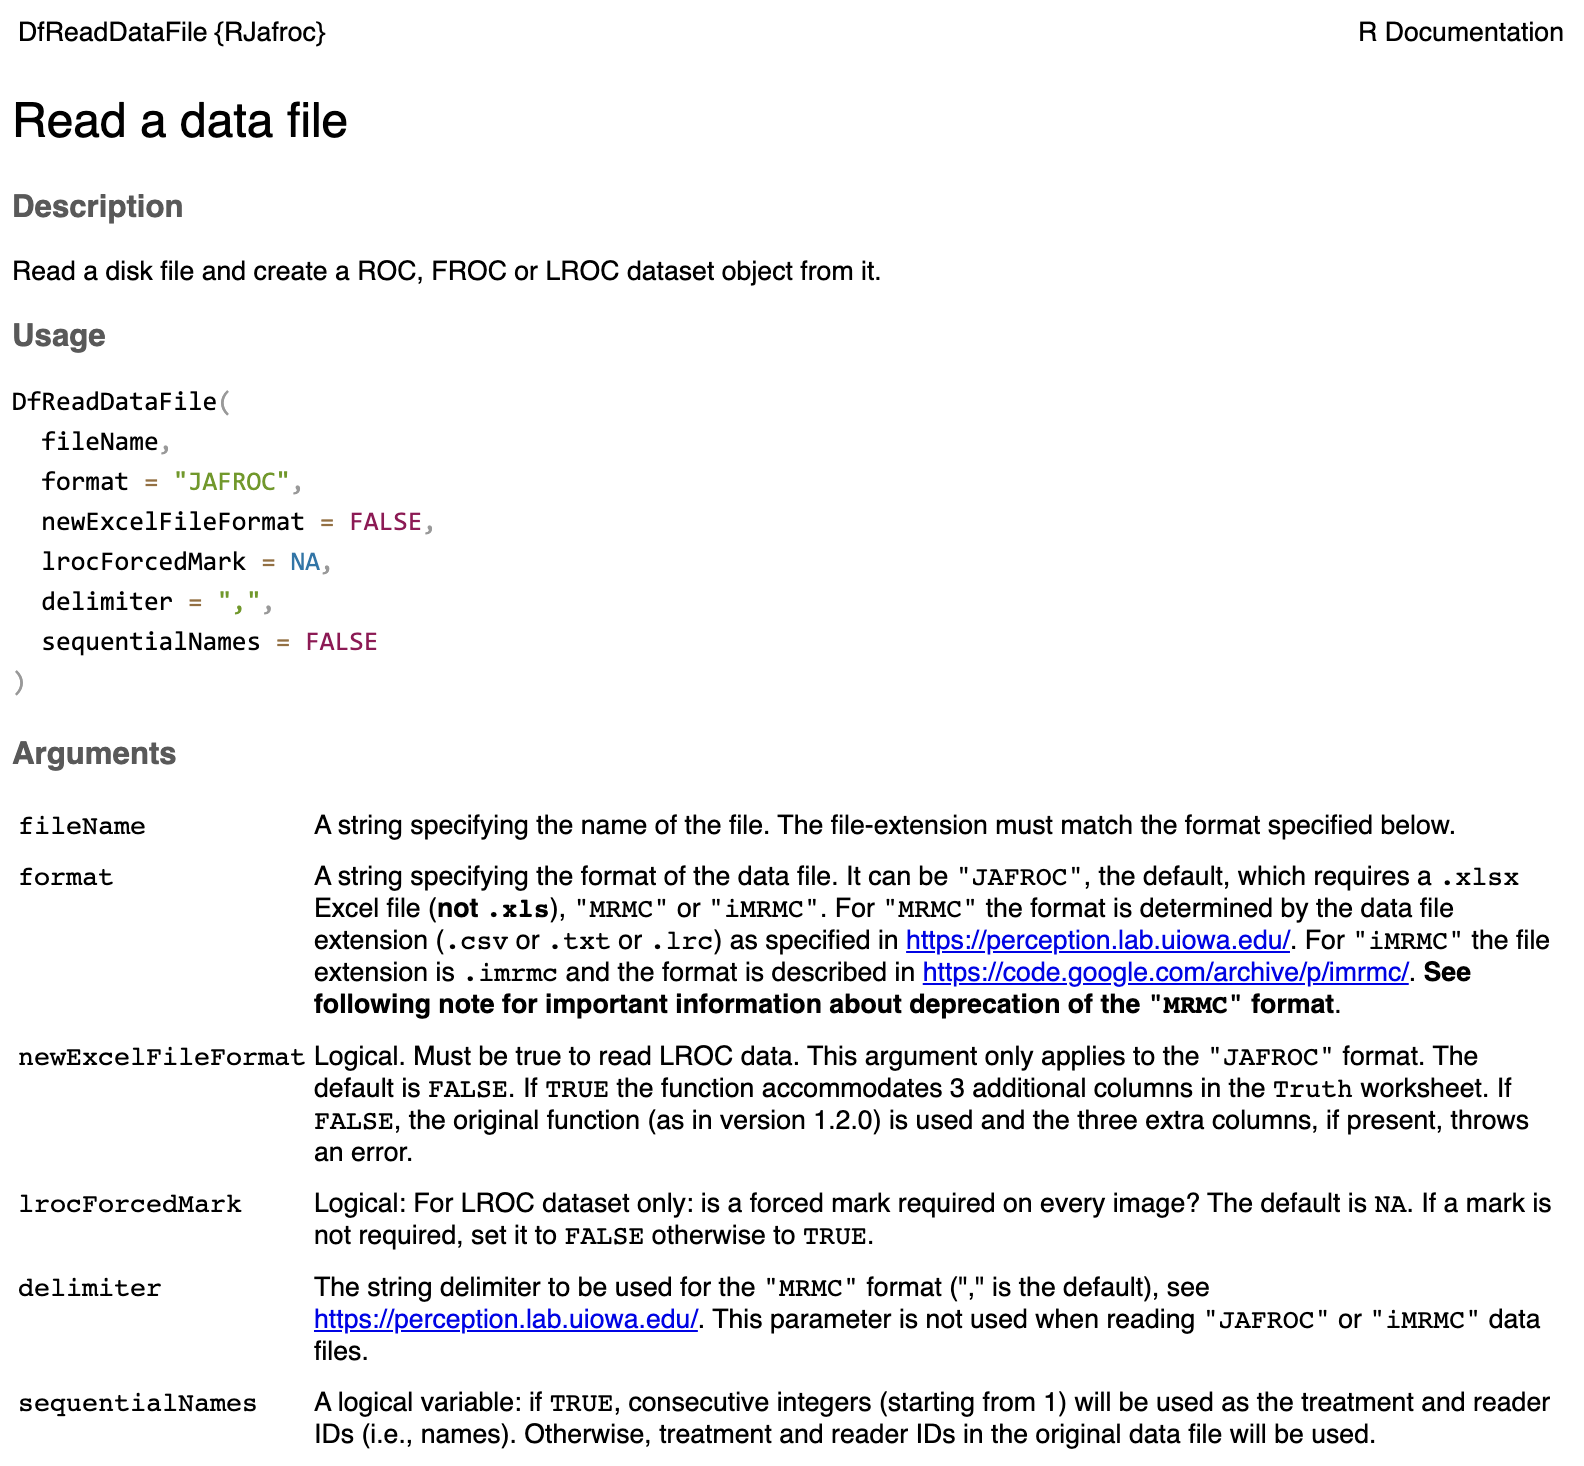
\includegraphics[width=22in]{images/roc-data-format/DfReadDataFile}

\hypertarget{quick-start-roc-excel}{%
\section{Three worksheets in the Excel data file}\label{quick-start-roc-excel}}

\begin{itemize}
\item
  The illustrations in this chapter are for Excel file \texttt{R/quick-start/rocCr.xlsx} in the project directory. I assume the reader has forked the \texttt{RJafrocQuickStart} repository. See Section @ref(\#quick-start-index-how-to-access-files) for how to get this file, and all other files and code in this \texttt{bookdown} book, on your computer.
\item
  This is a \emph{toy file}, i.e., a small made-up dataset used to illustrate essential features of the data format.
\item
  The Excel file has three worksheets: \texttt{Truth}, \texttt{NL} (or \texttt{FP}) and \texttt{LL} (or \texttt{TP}). The worksheet names are case insensitive.
\end{itemize}

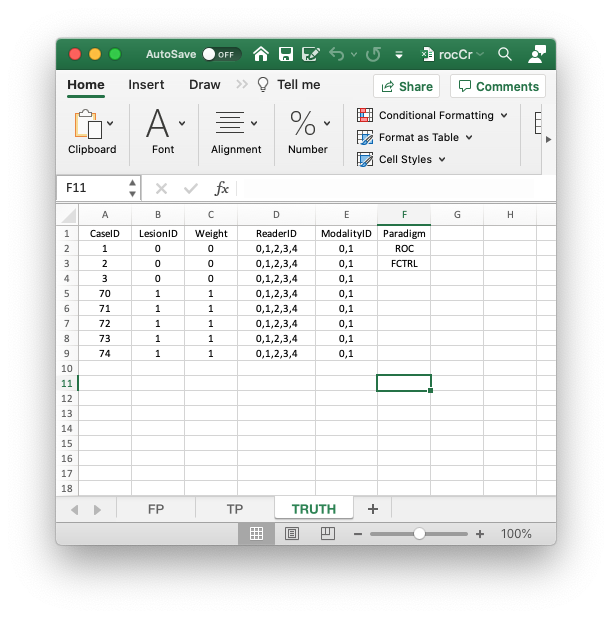
\includegraphics[width=1\textwidth,height=\textheight]{images/quick-start/rocCrTruth.png}

\hypertarget{quick-start-roc-truth}{%
\subsection{\texorpdfstring{The \texttt{Truth} worksheet}{The Truth worksheet}}\label{quick-start-roc-truth}}

The \texttt{Truth} worksheet shown above contains 6 columns: \texttt{CaseID}, \texttt{LesionID}, \texttt{Weight}, \texttt{ReaderID}, \texttt{ModalityID} and \texttt{Paradigm}. These names are case sensitive.

\begin{enumerate}
\def\labelenumi{\arabic{enumi}.}
\item
  \texttt{CaseID}: \textbf{unique integers}, one per case, representing the cases in the dataset. In the current dataset, the non-diseased cases are labeled \texttt{1}, \texttt{2} and \texttt{3}, while the diseased cases are labeled \texttt{70}, \texttt{71}, \texttt{72}, \texttt{73} and \texttt{74}. The values do not have to be consecutive integers; they need not be ordered; the only requirement is that they be unique integers.
\item
  \texttt{LesionID}: integers 0 or 1, with each 0 representing a non-diseased case and each 1 representing a diseased case.
\item
  \texttt{Weight}: this field is not used for ROC data.
\item
  \texttt{ReaderID}: a \textbf{comma-separated} string containing the reader (i.e., radiologist or observer) labels, each represented by a \textbf{unique integer}, that have interpreted the case. In the example shown below each cell has the value \texttt{0,\ 1,\ 2,\ 3,\ 4} meaning each of these readers has interpreted all cases. With multiple readers each cell in this column has to be text formatted as otherwise Excel will not accept it. Select the worksheet, then \texttt{Format} - \texttt{Cells} - \texttt{Number} - \texttt{Text} - \texttt{OK}.
\item
  \texttt{ModalityID}: a comma-separated string containing the modality labels, each represented by a \textbf{unique integer}. In the example each cell has the value \texttt{0,\ 1} meaning this is a two-modality study. As above, with multiple modalities each cell has to be text formatted as otherwise Excel will not accept it.
\item
  \texttt{Paradigm}: this column contains two cells, \texttt{ROC} and \texttt{FCTRL}. It means that this is an ROC dataset and the study design is factorial (or fully-crossed), i.e., each reader interprets each case in each modality.
\end{enumerate}

\hypertarget{quick-start-roc-truth-comments}{%
\subsection{\texorpdfstring{Comments on the \texttt{Truth} worksheet}{Comments on the Truth worksheet}}\label{quick-start-roc-truth-comments}}

There are 5 diseased cases in the dataset (the number of 1's in the \texttt{LesionID} column of the \texttt{Truth} worksheet). There are 3 non-diseased cases in the dataset (the number of 0's in the \texttt{LesionID} column). There are 5 readers in the dataset (each cell in the \texttt{ReaderID} column contains the string \texttt{0,\ 1,\ 2,\ 3,\ 4}). There are 2 modalities in the dataset (each cell in the \texttt{ModalityID} column contains the string \texttt{0,\ 1}).

\hypertarget{quick-start-roc-fp}{%
\subsection{The FP/NL worksheet}\label{quick-start-roc-fp}}

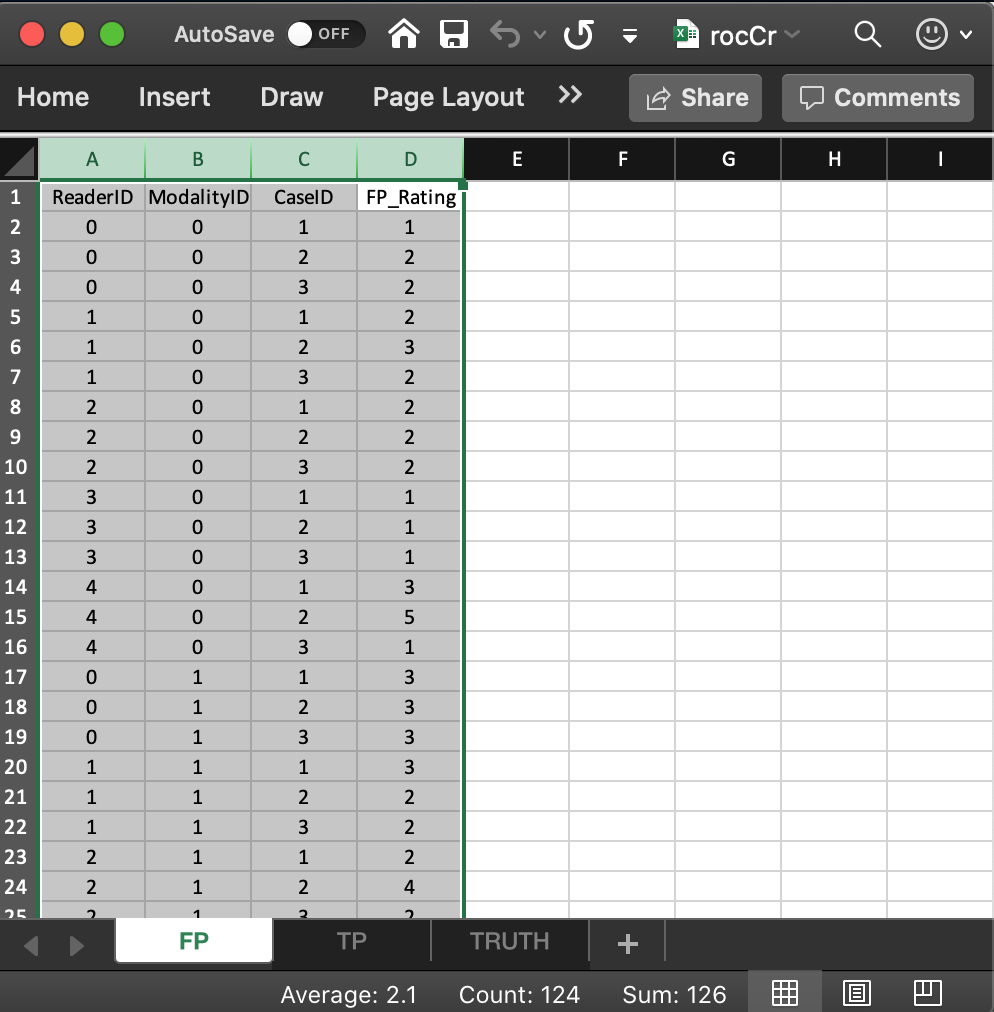
\includegraphics[width=1\textwidth,height=\textheight]{images/quick-start/rocCrFp.png}

It consists of 4 columns, each of length 30 (i.e., \# of modalities x number of readers x number of non-diseased cases). The (case sensitive) column names and meanings are as follows:

\begin{enumerate}
\def\labelenumi{\arabic{enumi}.}
\item
  \texttt{ReaderID}: the reader labels: \texttt{0}, \texttt{1}, \texttt{2}, \texttt{3} and \texttt{4}. Each reader label occurs 6 times (i.e., \# of modalities x number of non-diseased cases).
\item
  \texttt{ModalityID}: the modality or treatment labels: \texttt{0} and \texttt{1}. Each label occurs 15 times (i.e., \# of readers x number of non-diseased cases).
\item
  \texttt{CaseID}: the case labels for non-diseased cases: \texttt{1}, \texttt{2} and \texttt{3}. Each label occurs 10 times (i.e., \# of modalities x \# of readers). The label of a diseased case cannot occur in the FP worksheet. If it does the software generates an error.
\item
  \texttt{FP\_Rating}: the (floating point) ratings of non-diseased cases. Each row of this worksheet contains a rating corresponding to the values of \texttt{ReaderID}, \texttt{ModalityID} and \texttt{CaseID} for that row.
\end{enumerate}

\hypertarget{quick-start-roc-tp}{%
\subsection{The TP/LL worksheet}\label{quick-start-roc-tp}}

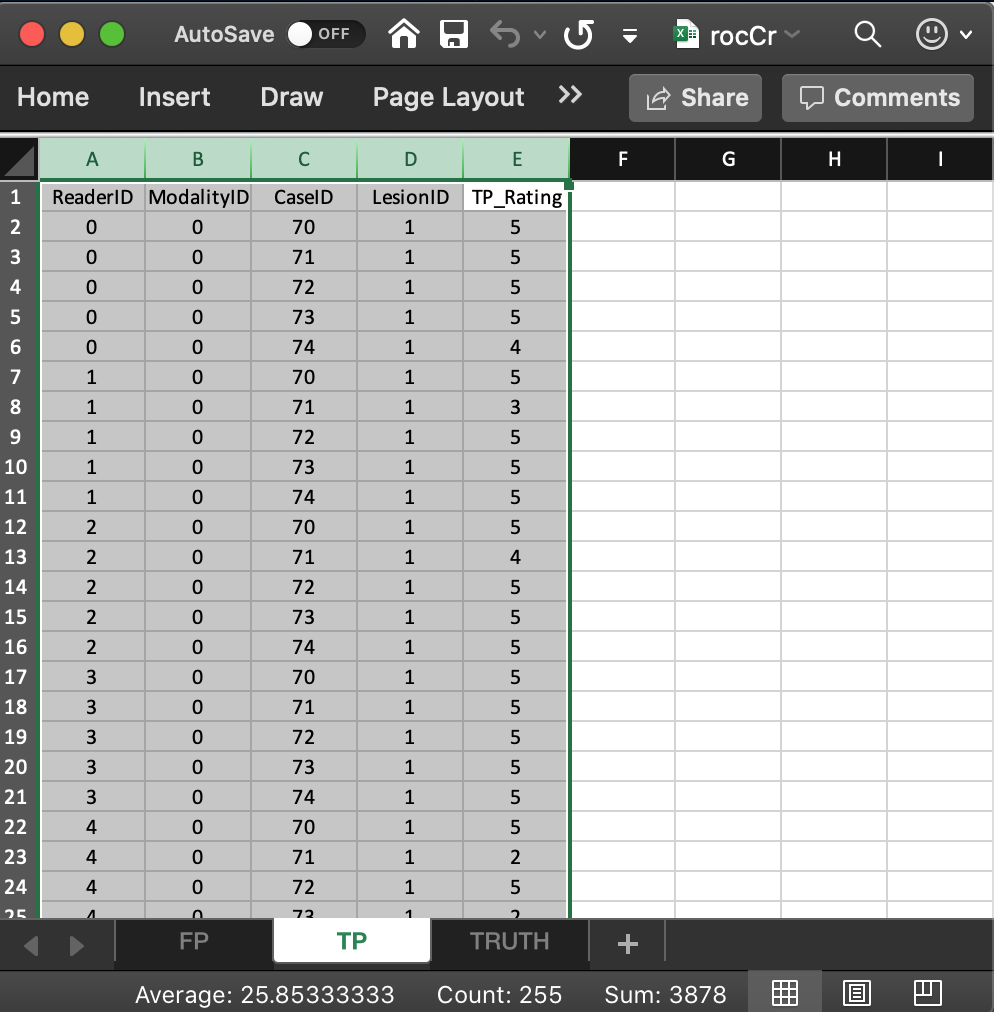
\includegraphics[width=1\textwidth,height=\textheight]{images/quick-start/rocCrTp.png}

It consists of 5 columns, each of length 50 (i.e., \# of modalities x number of readers x number of diseased cases). The (case sensitive) column names and meanings are as follows:

\begin{enumerate}
\def\labelenumi{\arabic{enumi}.}
\item
  \texttt{ReaderID}: the reader labels: \texttt{0}, \texttt{1}, \texttt{2}, \texttt{3} and \texttt{4}. Each reader label occurs 10 times (i.e., \# of modalities x number of diseased cases).
\item
  \texttt{ModalityID}: the modality or treatment labels: \texttt{0} and \texttt{1}. Each label occurs 25 times (i.e., \# of readers x number of diseased cases).
\item
  \texttt{LesionID}: For an ROC dataset this column contains fifty 1's (each diseased case has one lesion).
\item
  \texttt{CaseID}: the case labels for non-diseased cases: \texttt{70}, \texttt{71}, \texttt{72}, \texttt{73} and \texttt{74}. Each label occurs 10 times (i.e., \# of modalities x \# of readers). For an ROC dataset the label of a non-diseased case cannot occur in the TP worksheet. If it does the software generates an error.
\item
  \texttt{TP\_Rating}: the (floating point) ratings of diseased cases. Each row of this worksheet contains a rating corresponding to the values of \texttt{ReaderID}, \texttt{ModalityID}, \texttt{LesionID} and \texttt{CaseID} for that row.
\end{enumerate}

\hypertarget{quick-start-roc-read}{%
\section{Reading the Excel file}\label{quick-start-roc-read}}

The following code uses the function \texttt{DfReadDataFile} to read the Excel file and save it to object \texttt{x}.

\begin{Shaded}
\begin{Highlighting}[]
\NormalTok{x }\OtherTok{\textless{}{-}} \FunctionTok{DfReadDataFile}\NormalTok{(}\StringTok{"R/quick{-}start/rocCr.xlsx"}\NormalTok{, }\AttributeTok{newExcelFileFormat =} \ConstantTok{TRUE}\NormalTok{)}
\end{Highlighting}
\end{Shaded}

\begin{itemize}
\item
  \texttt{newExcelFileFormat} is set to \texttt{TRUE} as otherwise columns D - F in the \texttt{Truth} worksheet are ignored and the dataset is assumed to be factorial, with \texttt{dataType} ``automatically'' determined from the contents of the FP and TP worksheets. \footnote{The assumptions underlying the ``automatic'' determination could be defeated by data entry errors.}
\item
  Flag \texttt{newExcelFileFormat\ =\ FALSE}, the default, is for compatibility with the original JAFROC format Excel format, which did not have columns D - F in the \texttt{Truth} worksheet. Its usage is deprecated.
\end{itemize}

\hypertarget{quick-start-roc-structure-dataset}{%
\section{Structure of dataset object}\label{quick-start-roc-structure-dataset}}

Most users will not need to be concerned with the internal structure of the dataset object \texttt{x}. For those interested in it, for my reference, and for ease of future maintenance of the software, this is deferred to Section \ref{dataset-object-details-structure-roc-dataset}.

\hypertarget{quick-start-froc-data-format}{%
\chapter{FROC data format}\label{quick-start-froc-data-format}}

\hypertarget{quick-start-froc-how-much-finished}\label{quick-start-froc-how-much-finished}}

\hypertarget{quick-start-froc-data-intro}{%
\section{Introduction}\label{quick-start-froc-data-intro}}

The purpose of this chapter is to explain the format of the FROC Excel file and how to read this file into a dataset object suitable for analysis using the \texttt{RJafroc} package.

In the FROC paradigm the observer assigns a rating and a location to suspicious regions in images that exceed the reporting threshold. As an example a CAD algorithm may find tens of suspicious regions in each image but the algorithm designer only shows those regions (typically one or two) whose confidence levels exceed the chosen threshold.

The chapter is illustrated with a toy data file, \texttt{R/quick-start/frocCr.xlsx} in which readers `0', `1' and `2' interpret 8 cases in two modalities, `0' and `1'. The design is `factorial', abbreviated to \texttt{FCTRL} in the software; this is also termed a `fully-crossed' design. The Excel file has three worksheets named \texttt{Truth}, \texttt{NL} (or \texttt{FP}) and \texttt{LL} (or \texttt{TP}). These names are case-insensitive.

\hypertarget{quick-start-froc-data-truth}{%
\section{\texorpdfstring{The \texttt{Truth} worksheet}{The Truth worksheet}}\label{quick-start-froc-data-truth}}

\includegraphics[width=1\textwidth,height=\textheight]{images/quick-start/frocCrTruth.png}

The \texttt{Truth} worksheet contains 6 columns: \texttt{CaseID}, \texttt{LesionID}, \texttt{Weight}, \texttt{ReaderID}, \texttt{ModalityID} and \texttt{Paradigm}. Since a diseased case may have more than one lesion, the first five columns contain \textbf{at least} as many rows as there are cases in the dataset. There are 8 cases (`1',`2',`3',`70',`71',`72',`73' and `74') in the dataset and 12 rows in the \texttt{Truth} worksheet, because some of the diseased cases contain more than one lesion.

\begin{enumerate}
\def\labelenumi{\arabic{enumi}.}
\item
  \texttt{CaseID}: unique \textbf{integers} representing the individual cases in the dataset: e.g., `1', `2', `3', the 3 non-diseased cases and `70', `71', `72', `73', `74', the 5 diseased cases. The ordering of the numbers is inconsequential. \footnote{\texttt{CaseID} should not be so large that it cannot be represented in Excel by an integer; to be safe use unsigned short 8-bit integers.}
\item
  \texttt{LesionID}: non-negative integers 0, 1, 2, \ldots, where:

  \begin{itemize}
  \tightlist
  \item
    Each 0 represents a non-diseased case, e.g., this field is zero for non-diseased cases `1', `2' and `3'.
  \item
    Each 1 represents the \emph{first} lesion in a diseased case, 2 represents the \emph{second} lesion, if present, and so on.
  \end{itemize}
\item
  \texttt{Weight} or clinical importance associated with lesion:

  \begin{itemize}
  \tightlist
  \item
    It is 0 for each non-diseased case,
  \item
    For each diseased case the values must sum to unity.
  \item
    A shortcut to assigning equal weights to all lesions in a case is to fill the \texttt{Weight} column with zeroes.
  \end{itemize}
\item
  \texttt{ReaderID}: see Section \ref{quick-start-roc-truth}.
\item
  \texttt{ModalityID}: see Section \ref{quick-start-roc-truth}.
\item
  \texttt{Paradigm}: see Section \ref{quick-start-roc-truth}.
\end{enumerate}

\hypertarget{quick-start-froc-truth-comments}{%
\subsection{\texorpdfstring{Comments on the \texttt{Truth} worksheet}{Comments on the Truth worksheet}}\label{quick-start-froc-truth-comments}}

There are 3 non-diseased cases in the dataset (the number of 0's in the \texttt{LesionID} column). There are 5 diseased cases in the dataset (the number of 1's in the \texttt{LesionID} column). There are 3 readers in the dataset labeled `0, 1, 2'. There are 2 modalities in the dataset labeled `0, 1'. Diseased case \texttt{70} has two lesions, with \texttt{LesionID}s `1' and `2' and weights 0.3 and 0.7, respectively. Diseased case \texttt{71} has one lesion with \texttt{LesionID} = 1 and \texttt{Weight} = 1. Diseased case \texttt{72} has three lesions with \texttt{LesionID}s 1, 2 and 3 and weights 1/3 each. Diseased case \texttt{73} has two lesions, with \texttt{LesionID}s 1, and 2 and weights 0.1 and 0.9, respectively. Diseased case \texttt{74} has one lesion, with \texttt{LesionID} = 1 and \texttt{Weight} = 1. Note that \texttt{LesionID}s \emph{identify} the lesions - for example, a lesion with high morbidity may be labeled \texttt{LesionID} = 1 and assigned weight 0.9 while a second lower morbidity lesion on the same case may be assigned \texttt{LesionID} = 2 and weight 0.1. In this example reversing the lesion IDs would lead to incorrect weight assignments.

\hypertarget{quick-start-froc-data-fp}{%
\section{The FP ratings}\label{quick-start-froc-data-fp}}

These are found in the \texttt{FP} or \texttt{NL} worksheet.

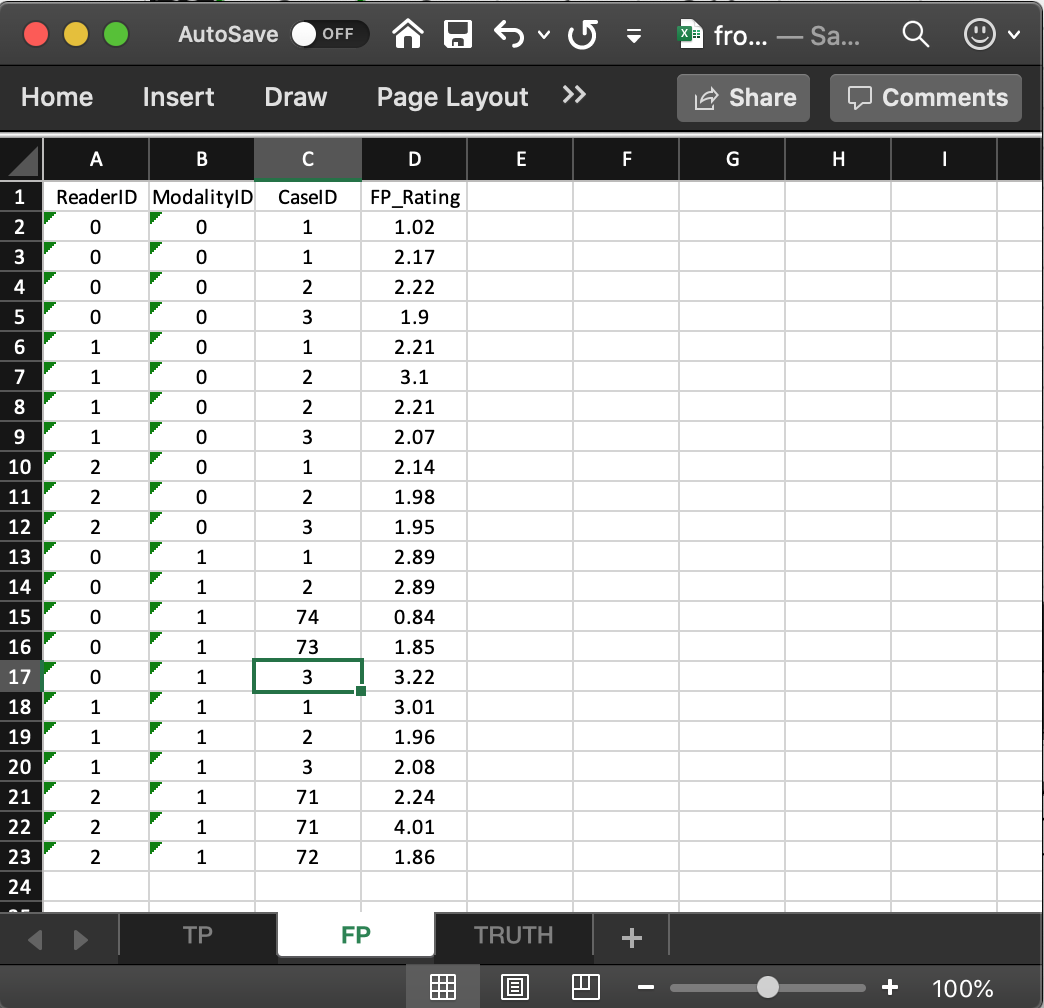
\includegraphics[width=1\textwidth,height=\textheight]{images/quick-start/frocCrNL.png}

It consists of 4 columns of equal length. The common length is an integer random variable \(\ge 0\). It could be zero if the dataset has no NL marks (a possibility if the lesions are easy to find or the observer has perfect performance). In this example the common length is 22. The common length is a-priori unpredictable; for example if the dataset has many FPs it could be large.

\begin{enumerate}
\def\labelenumi{\arabic{enumi}.}
\item
  \texttt{ReaderID}: the reader labels: these must be one of \texttt{0}, \texttt{1}, or \texttt{2} as declared in the \texttt{Truth} worksheet.
\item
  \texttt{ModalityID}: the modality labels: must be one of \texttt{0} or \texttt{1} as declared in the \texttt{Truth} worksheet.
\item
  \texttt{CaseID}: the labels of cases with \texttt{NL} marks. These must be one of \texttt{1}, \texttt{2}, \texttt{3}, \texttt{70}, \texttt{71}, \texttt{72}, \texttt{73}, \texttt{74} as declared in the \texttt{Truth} worksheet. In the FROC paradigm \texttt{NL} events can occur on non-diseased \textbf{and} diseased cases.
\item
  \texttt{FP\_Rating}: the floating point ratings of \texttt{NL} marks. Each cell contains the rating corresponding to the values of \texttt{ReaderID}, \texttt{ModalityID} and \texttt{CaseID} for that row.
\end{enumerate}

\hypertarget{quick-start-roc-fp-comments}{%
\subsection{\texorpdfstring{Comments on the \texttt{FP} worksheet}{Comments on the FP worksheet}}\label{quick-start-roc-fp-comments}}

\begin{itemize}
\item
  For \texttt{ModalityID} 0, \texttt{ReaderID} 0 and \texttt{CaseID} 1 (the first non-diseased case declared in the \texttt{Truth} worksheet), there is a single \texttt{NL} mark that was rated 1.02, corresponding to row 2 of the \texttt{FP} worksheet.
\item
  Diseased cases with \texttt{NL} marks are also recorded in the \texttt{FP} worksheet. Some examples are seen at rows 15, 16 and 21, 22, 23. Rows 21 and 22 show that \texttt{caseID} = 71 got two \texttt{NL} marks, rated 2.24, 4.01.
\item
  Since this is the \emph{only} case with two NL marks, it determines the length of the fourth dimension of the \texttt{x\$ratings\$NL}, which is 2 in this example. Absent this case, the length would have been one. The case with the most \texttt{NL} marks determines the length of the fourth dimension of \texttt{x\$ratings\$NL}. The reader should confirm that the ratings in \texttt{x\$ratings\$NL} reflect the contents of the \texttt{FP} worksheet.
\end{itemize}

\hypertarget{quick-start-froc-data-tp}{%
\section{The TP ratings}\label{quick-start-froc-data-tp}}

These are found in the \texttt{TP} or \texttt{LL} worksheet, see below.

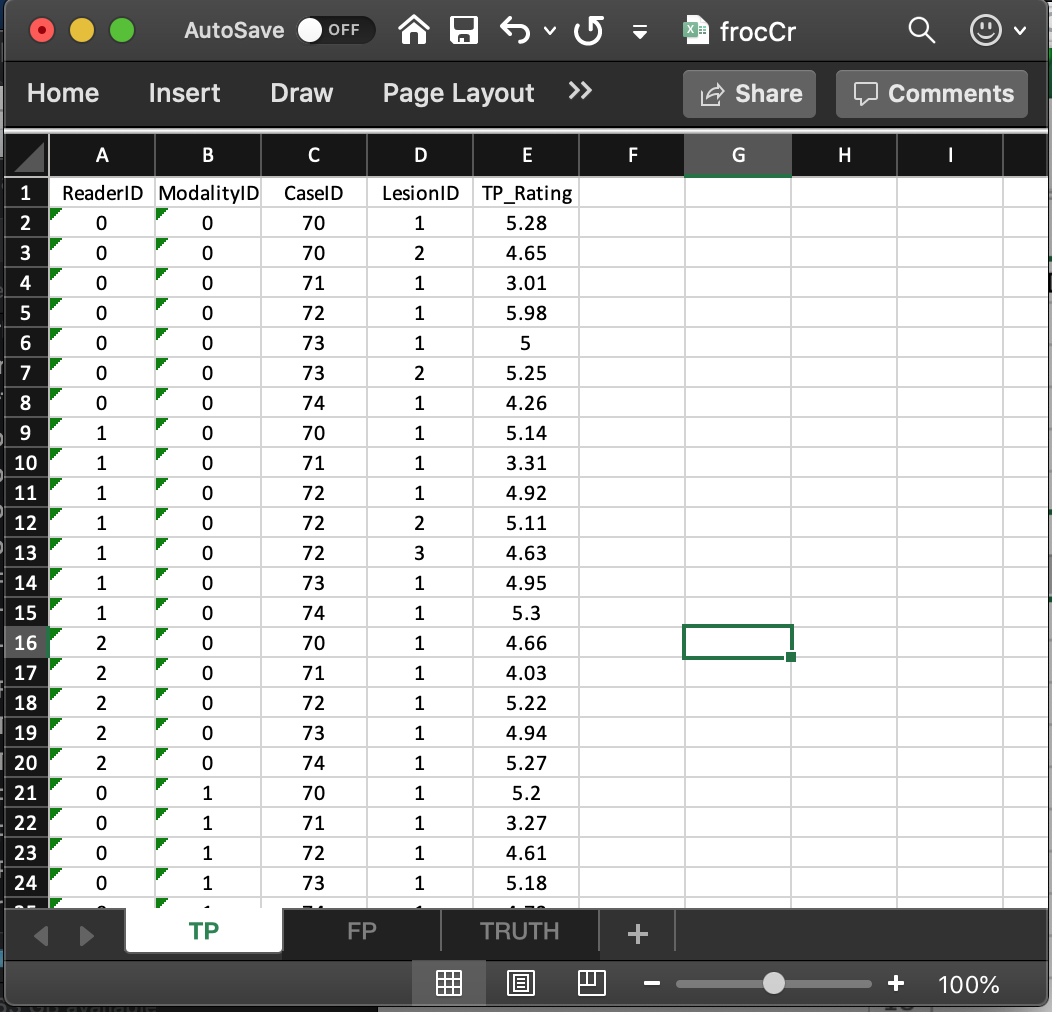
\includegraphics[width=1\textwidth,height=\textheight]{images/quick-start/frocCrLL.png}

This worksheet can only have diseased cases. The presence of a non-diseased case will generate an error. The common vertical length, 31 in this example, is a-priori unpredictable (as some lesions may not be marked). The maximum possible length, assuming every lesion is marked for each modality, reader and diseased case, is 9 X 2 X 3 = 54. The 9 comes from the total number of non-zero entries in the \texttt{LesionID} column of the \texttt{Truth} worksheet, the 2 from the number of modalities and 3 from the number of readers.

The fact that the actual length (31) is smaller than the maximum length (54) means that there are combinations of modality, reader and diseased cases on which some lesions were not marked.

As examples, line 2 in the worksheet, the first lesion in \texttt{CaseID} equal to \texttt{70} was marked (and rated 5.28) in \texttt{ModalityID} \texttt{0} and \texttt{ReaderID} \texttt{0}. Line 3 in the worksheet, the second lesion in \texttt{CaseID} equal to \texttt{70} was also marked (and rated 4.65) in \texttt{ModalityID} \texttt{0} and \texttt{ReaderID} \texttt{0}. However, lesions 2 and 3 in \texttt{CaseID} = 72 were not marked (line 5 in the worksheet indicates that for this modality-reader-case combination only the first lesion was marked). The reader should confirm that the ratings in \texttt{x\$ratings\$LL} reflect the contents of the \texttt{TP} worksheet.

\hypertarget{quick-start-froc-data-structure}{%
\section{Reading the FROC dataset}\label{quick-start-froc-data-structure}}

The example shown above corresponds to file \texttt{R/quick-start/frocCr.xlsx} in the project directory. The next code reads this file into an \texttt{R} object \texttt{x}.

\begin{Shaded}
\begin{Highlighting}[]
\NormalTok{frocCr }\OtherTok{\textless{}{-}} \StringTok{"R/quick{-}start/frocCr.xlsx"}
\NormalTok{x }\OtherTok{\textless{}{-}} \FunctionTok{DfReadDataFile}\NormalTok{(frocCr, }\AttributeTok{newExcelFileFormat =} \ConstantTok{TRUE}\NormalTok{)}
\FunctionTok{str}\NormalTok{(x)}
\CommentTok{\#\textgreater{} List of 3}
\CommentTok{\#\textgreater{}  $ ratings     :List of 3}
\CommentTok{\#\textgreater{}   ..$ NL   : num [1:2, 1:3, 1:8, 1:2] 1.02 2.89 2.21 3.01 2.14 ...}
\CommentTok{\#\textgreater{}   ..$ LL   : num [1:2, 1:3, 1:5, 1:3] 5.28 5.2 5.14 4.77 4.66 4.87 3.01 3.27 3.31 3.19 ...}
\CommentTok{\#\textgreater{}   ..$ LL\_IL: logi NA}
\CommentTok{\#\textgreater{}  $ lesions     :List of 3}
\CommentTok{\#\textgreater{}   ..$ perCase: int [1:5] 2 1 3 2 1}
\CommentTok{\#\textgreater{}   ..$ IDs    : num [1:5, 1:3] 1 1 1 1 1 ...}
\CommentTok{\#\textgreater{}   ..$ weights: num [1:5, 1:3] 0.3 1 0.333 0.1 1 ...}
\CommentTok{\#\textgreater{}  $ descriptions:List of 7}
\CommentTok{\#\textgreater{}   ..$ fileName     : chr "frocCr"}
\CommentTok{\#\textgreater{}   ..$ type         : chr "FROC"}
\CommentTok{\#\textgreater{}   ..$ name         : logi NA}
\CommentTok{\#\textgreater{}   ..$ truthTableStr: num [1:2, 1:3, 1:8, 1:4] 1 1 1 1 1 1 1 1 1 1 ...}
\CommentTok{\#\textgreater{}   ..$ design       : chr "FCTRL"}
\CommentTok{\#\textgreater{}   ..$ modalityID   : Named chr [1:2] "0" "1"}
\CommentTok{\#\textgreater{}   .. ..{-} attr(*, "names")= chr [1:2] "0" "1"}
\CommentTok{\#\textgreater{}   ..$ readerID     : Named chr [1:3] "0" "1" "2"}
\CommentTok{\#\textgreater{}   .. ..{-} attr(*, "names")= chr [1:3] "0" "1" "2"}
\end{Highlighting}
\end{Shaded}

This follows the general description in Chapter \ref{quick-start-roc}. The differences are described below.

\begin{itemize}
\item
  The \texttt{x\$descriptions\$type} member indicates that this is an \texttt{FROC} dataset.
\item
  The \texttt{x\$lesions\$perCase} member is a vector whose contents reflect the number of lesions in each diseased case, i.e., 2, 1, 3, 2, 1 in the current example.
\item
  The \texttt{x\$lesions\$IDs} member indicates the labeling of the lesions in each diseased case.
\end{itemize}

\begin{Shaded}
\begin{Highlighting}[]
\NormalTok{x}\SpecialCharTok{$}\NormalTok{lesions}\SpecialCharTok{$}\NormalTok{IDs}
\CommentTok{\#\textgreater{}      [,1] [,2] [,3]}
\CommentTok{\#\textgreater{} [1,]    1    2 {-}Inf}
\CommentTok{\#\textgreater{} [2,]    1 {-}Inf {-}Inf}
\CommentTok{\#\textgreater{} [3,]    1    2    3}
\CommentTok{\#\textgreater{} [4,]    1    2 {-}Inf}
\CommentTok{\#\textgreater{} [5,]    1 {-}Inf {-}Inf}
\end{Highlighting}
\end{Shaded}

\begin{itemize}
\item
  This shows that the lesions on the first diseased case are labeled `1' and `2'. The \texttt{-Inf} is a filler used to denote a missing value. The second diseased case has one lesion labeled `1'. The third diseased case has three lesions labeled `1', `2' and `3', etc.
\item
  The \texttt{lesionWeight} member is the clinical importance of each lesion. Lacking specific clinical reasons, the lesions should be equally weighted; this is \emph{not} true for this toy dataset.
\end{itemize}

\begin{Shaded}
\begin{Highlighting}[]
\NormalTok{x}\SpecialCharTok{$}\NormalTok{lesions}\SpecialCharTok{$}\NormalTok{weights}
\CommentTok{\#\textgreater{}           [,1]      [,2]      [,3]}
\CommentTok{\#\textgreater{} [1,] 0.3000000 0.7000000      {-}Inf}
\CommentTok{\#\textgreater{} [2,] 1.0000000      {-}Inf      {-}Inf}
\CommentTok{\#\textgreater{} [3,] 0.3333333 0.3333333 0.3333333}
\CommentTok{\#\textgreater{} [4,] 0.1000000 0.9000000      {-}Inf}
\CommentTok{\#\textgreater{} [5,] 1.0000000      {-}Inf      {-}Inf}
\end{Highlighting}
\end{Shaded}

\begin{itemize}
\item
  The first diseased case has two lesions, the first has weight 0.3 and the second has weight 0.7.
\item
  The second diseased case has one lesion with weight 1.
\item
  The third diseased case has three equally weighted lesions, each with weight 1/3. Etc.
\end{itemize}

\hypertarget{quick-start-froc-data-distribution-diseased-cases}{%
\section{On the distribution of numbers of lesions in diseased cases}\label{quick-start-froc-data-distribution-diseased-cases}}

Consider a much larger real dataset, \texttt{dataset11}, with structure as shown below (for descriptions of all embedded datasets see Chapter \ref{datasets}):

\begin{Shaded}
\begin{Highlighting}[]
\NormalTok{x }\OtherTok{\textless{}{-}}\NormalTok{ dataset11}
\FunctionTok{str}\NormalTok{(x)}
\CommentTok{\#\textgreater{} List of 3}
\CommentTok{\#\textgreater{}  $ ratings     :List of 3}
\CommentTok{\#\textgreater{}   ..$ NL   : num [1:4, 1:5, 1:158, 1:4] {-}Inf {-}Inf {-}Inf {-}Inf {-}Inf ...}
\CommentTok{\#\textgreater{}   ..$ LL   : num [1:4, 1:5, 1:115, 1:20] {-}Inf {-}Inf {-}Inf {-}Inf {-}Inf ...}
\CommentTok{\#\textgreater{}   ..$ LL\_IL: logi NA}
\CommentTok{\#\textgreater{}  $ lesions     :List of 3}
\CommentTok{\#\textgreater{}   ..$ perCase: int [1:115] 6 4 7 1 3 3 3 8 11 2 ...}
\CommentTok{\#\textgreater{}   ..$ IDs    : num [1:115, 1:20] 1 1 1 1 1 1 1 1 1 1 ...}
\CommentTok{\#\textgreater{}   ..$ weights: num [1:115, 1:20] 0.167 0.25 0.143 1 0.333 ...}
\CommentTok{\#\textgreater{}  $ descriptions:List of 7}
\CommentTok{\#\textgreater{}   ..$ fileName     : chr "dataset11"}
\CommentTok{\#\textgreater{}   ..$ type         : chr "FROC"}
\CommentTok{\#\textgreater{}   ..$ name         : chr "DOBBINS{-}1"}
\CommentTok{\#\textgreater{}   ..$ truthTableStr: num [1:4, 1:5, 1:158, 1:21] 1 1 1 1 1 1 1 1 1 1 ...}
\CommentTok{\#\textgreater{}   ..$ design       : chr "FCTRL"}
\CommentTok{\#\textgreater{}   ..$ modalityID   : Named chr [1:4] "1" "2" "3" "4"}
\CommentTok{\#\textgreater{}   .. ..{-} attr(*, "names")= chr [1:4] "1" "2" "3" "4"}
\CommentTok{\#\textgreater{}   ..$ readerID     : Named chr [1:5] "1" "2" "3" "4" ...}
\CommentTok{\#\textgreater{}   .. ..{-} attr(*, "names")= chr [1:5] "1" "2" "3" "4" ...}
\end{Highlighting}
\end{Shaded}

Focus for now in the 115 diseased cases. The numbers of lesions in these cases is contained in \texttt{x\$lesions\$perCase}.

\begin{Shaded}
\begin{Highlighting}[]
\NormalTok{x}\SpecialCharTok{$}\NormalTok{lesions}\SpecialCharTok{$}\NormalTok{perCase}
\CommentTok{\#\textgreater{}   [1]  6  4  7  1  3  3  3  8 11  2  4  6  2 16  5  2  8  3  4  7 11  1  4  3  4}
\CommentTok{\#\textgreater{}  [26]  4  7  3  2  5  2  2  7  6  6  4 10 20 12  6  4  7 12  5  1  1  5  1  2  8}
\CommentTok{\#\textgreater{}  [51]  3  1  2  2  3  2  8 16 10  1  2  2  6  3  2  2  4  6 10 11  1  2  6  2  4}
\CommentTok{\#\textgreater{}  [76]  5  2  9  6  6  8  3  8  7  1  1  6  3  2  1  9  8  8  2  2 12  1  1  1  1}
\CommentTok{\#\textgreater{} [101]  1  3  1  2  2  1  1  1  1  3  1  1  1  2  1}
\end{Highlighting}
\end{Shaded}

For example, the first diseased case contains 6 lesions, the second contains 4 lesions, the third contains 7 lesions, etc. and the last diseased case contains 1 lesion. To get an idea of the distribution of the numbers of lesions per diseased cases, one could use the \texttt{which()} function:

\begin{Shaded}
\begin{Highlighting}[]
\ControlFlowTok{for}\NormalTok{ (el }\ControlFlowTok{in} \DecValTok{1}\SpecialCharTok{:}\FunctionTok{max}\NormalTok{(x}\SpecialCharTok{$}\NormalTok{lesions}\SpecialCharTok{$}\NormalTok{perCase)) }\FunctionTok{cat}\NormalTok{(}
  \StringTok{"number of diseased cases with"}\NormalTok{, el, }\StringTok{"lesions = "}\NormalTok{, }
  \FunctionTok{length}\NormalTok{(}\FunctionTok{which}\NormalTok{(x}\SpecialCharTok{$}\NormalTok{lesions}\SpecialCharTok{$}\NormalTok{perCase }\SpecialCharTok{==}\NormalTok{ el)), }\StringTok{"}\SpecialCharTok{\textbackslash{}n}\StringTok{"}\NormalTok{)}
\CommentTok{\#\textgreater{} number of diseased cases with 1 lesions =  25 }
\CommentTok{\#\textgreater{} number of diseased cases with 2 lesions =  23 }
\CommentTok{\#\textgreater{} number of diseased cases with 3 lesions =  13 }
\CommentTok{\#\textgreater{} number of diseased cases with 4 lesions =  10 }
\CommentTok{\#\textgreater{} number of diseased cases with 5 lesions =  5 }
\CommentTok{\#\textgreater{} number of diseased cases with 6 lesions =  11 }
\CommentTok{\#\textgreater{} number of diseased cases with 7 lesions =  6 }
\CommentTok{\#\textgreater{} number of diseased cases with 8 lesions =  8 }
\CommentTok{\#\textgreater{} number of diseased cases with 9 lesions =  2 }
\CommentTok{\#\textgreater{} number of diseased cases with 10 lesions =  3 }
\CommentTok{\#\textgreater{} number of diseased cases with 11 lesions =  3 }
\CommentTok{\#\textgreater{} number of diseased cases with 12 lesions =  3 }
\CommentTok{\#\textgreater{} number of diseased cases with 13 lesions =  0 }
\CommentTok{\#\textgreater{} number of diseased cases with 14 lesions =  0 }
\CommentTok{\#\textgreater{} number of diseased cases with 15 lesions =  0 }
\CommentTok{\#\textgreater{} number of diseased cases with 16 lesions =  2 }
\CommentTok{\#\textgreater{} number of diseased cases with 17 lesions =  0 }
\CommentTok{\#\textgreater{} number of diseased cases with 18 lesions =  0 }
\CommentTok{\#\textgreater{} number of diseased cases with 19 lesions =  0 }
\CommentTok{\#\textgreater{} number of diseased cases with 20 lesions =  1}
\end{Highlighting}
\end{Shaded}

This tells us that 25 cases contain 1 lesion. Likewise, 23 cases contain 2 lesions, etc.

\hypertarget{quick-start-froc-data-lesion-distribution}{%
\subsection{\texorpdfstring{Definition of \texttt{lesDistr} array}{Definition of lesDistr array}}\label{quick-start-froc-data-lesion-distribution}}

The histogram of the number of lesions per case, i.e., what is the fraction of (diseased) cases with 1 lesion, 2 lesions etc, can be calculated as follows:

\begin{Shaded}
\begin{Highlighting}[]
\ControlFlowTok{for}\NormalTok{ (el }\ControlFlowTok{in} \DecValTok{1}\SpecialCharTok{:}\FunctionTok{max}\NormalTok{(x}\SpecialCharTok{$}\NormalTok{lesions}\SpecialCharTok{$}\NormalTok{perCase)) }
  \FunctionTok{cat}\NormalTok{(}\StringTok{"fraction of diseased cases with"}\NormalTok{, el, }\StringTok{"lesions = "}\NormalTok{, }
  \FunctionTok{length}\NormalTok{(}\FunctionTok{which}\NormalTok{(x}\SpecialCharTok{$}\NormalTok{lesions}\SpecialCharTok{$}\NormalTok{perCase }\SpecialCharTok{==}\NormalTok{ el))}\SpecialCharTok{/}\FunctionTok{length}\NormalTok{(x}\SpecialCharTok{$}\NormalTok{ratings}\SpecialCharTok{$}\NormalTok{LL[}\DecValTok{1}\NormalTok{,}\DecValTok{1}\NormalTok{,,}\DecValTok{1}\NormalTok{]), }\StringTok{"}\SpecialCharTok{\textbackslash{}n}\StringTok{"}\NormalTok{)}
\CommentTok{\#\textgreater{} fraction of diseased cases with 1 lesions =  0.2173913 }
\CommentTok{\#\textgreater{} fraction of diseased cases with 2 lesions =  0.2 }
\CommentTok{\#\textgreater{} fraction of diseased cases with 3 lesions =  0.1130435 }
\CommentTok{\#\textgreater{} fraction of diseased cases with 4 lesions =  0.08695652 }
\CommentTok{\#\textgreater{} fraction of diseased cases with 5 lesions =  0.04347826 }
\CommentTok{\#\textgreater{} fraction of diseased cases with 6 lesions =  0.09565217 }
\CommentTok{\#\textgreater{} fraction of diseased cases with 7 lesions =  0.05217391 }
\CommentTok{\#\textgreater{} fraction of diseased cases with 8 lesions =  0.06956522 }
\CommentTok{\#\textgreater{} fraction of diseased cases with 9 lesions =  0.0173913 }
\CommentTok{\#\textgreater{} fraction of diseased cases with 10 lesions =  0.02608696 }
\CommentTok{\#\textgreater{} fraction of diseased cases with 11 lesions =  0.02608696 }
\CommentTok{\#\textgreater{} fraction of diseased cases with 12 lesions =  0.02608696 }
\CommentTok{\#\textgreater{} fraction of diseased cases with 13 lesions =  0 }
\CommentTok{\#\textgreater{} fraction of diseased cases with 14 lesions =  0 }
\CommentTok{\#\textgreater{} fraction of diseased cases with 15 lesions =  0 }
\CommentTok{\#\textgreater{} fraction of diseased cases with 16 lesions =  0.0173913 }
\CommentTok{\#\textgreater{} fraction of diseased cases with 17 lesions =  0 }
\CommentTok{\#\textgreater{} fraction of diseased cases with 18 lesions =  0 }
\CommentTok{\#\textgreater{} fraction of diseased cases with 19 lesions =  0 }
\CommentTok{\#\textgreater{} fraction of diseased cases with 20 lesions =  0.008695652}
\end{Highlighting}
\end{Shaded}

Fraction 0.217 of (diseased) cases contain 1 lesion, fraction 0.2 of (diseased) cases contain 2 lesions, etc.

This information is more readily obtained using the \texttt{RJafroc} function \texttt{UtilLesionDistrVector()} as shown next:

\begin{Shaded}
\begin{Highlighting}[]
\NormalTok{lesDistr }\OtherTok{\textless{}{-}} \FunctionTok{UtilLesionDistrVector}\NormalTok{(x)}
\NormalTok{lesDistr}
\CommentTok{\#\textgreater{}  [1] 0.217391304 0.200000000 0.113043478 0.086956522 0.043478261 0.095652174}
\CommentTok{\#\textgreater{}  [7] 0.052173913 0.069565217 0.017391304 0.026086957 0.026086957 0.026086957}
\CommentTok{\#\textgreater{} [13] 0.017391304 0.008695652}
\end{Highlighting}
\end{Shaded}

\begin{itemize}
\tightlist
\item
  TBA The \texttt{UtilLesionDistrVector()} function returns an array with two columns and number of rows equal to the number of \emph{distinct non-zero} values of lesions per case.
\item
  The first column contains the number of distinct non-zero values of lesions per case, 14 in the current example.
\item
  The second column contains the fraction of diseased cases with the number of lesions indicated in the first column.
\item
  The second column must sum to unity
\end{itemize}

\begin{Shaded}
\begin{Highlighting}[]
\FunctionTok{sum}\NormalTok{(}\FunctionTok{UtilLesionDistrVector}\NormalTok{(x))}
\CommentTok{\#\textgreater{} [1] 1}
\end{Highlighting}
\end{Shaded}

\begin{itemize}
\tightlist
\item
  The lesion distribution array will come in handy when it comes to predicting the operating characteristics from using the Radiological Search Model (RSM), as detailed in TBA Chapter 17.
\end{itemize}

\hypertarget{quick-start-froc-data-lesion-weights}{%
\section{\texorpdfstring{TBA Definition of \texttt{lesWghtDistr} array}{TBA Definition of lesWghtDistr array}}\label{quick-start-froc-data-lesion-weights}}

\begin{itemize}
\tightlist
\item
  This is returned by \texttt{UtilLesionWeightsDistr()}.
\item
  This contains the same number of rows as \texttt{lesDistr}.
\item
  The number of columns is one plus the number of rows as \texttt{lesDistr}.
\item
  The first column contains the number of distinct non-zero values of lesions per case, 14 in the current example.
\item
  The second through the last columns contain the weights of cases with number of lesions per case corresponding to row 1.
\item
  Missing values are filled with \texttt{-Inf}.
\end{itemize}

\begin{Shaded}
\begin{Highlighting}[]
\NormalTok{lesWghtDistr }\OtherTok{\textless{}{-}} \FunctionTok{UtilLesionWeightsMatrixDataset}\NormalTok{(x, }\AttributeTok{relWeights =} \DecValTok{0}\NormalTok{)}
\FunctionTok{cat}\NormalTok{(}\StringTok{"dim(lesDistr) ="}\NormalTok{, }\FunctionTok{dim}\NormalTok{(lesDistr),}\StringTok{"}\SpecialCharTok{\textbackslash{}n}\StringTok{"}\NormalTok{)}
\CommentTok{\#\textgreater{} dim(lesDistr) =}
\FunctionTok{cat}\NormalTok{(}\StringTok{"dim(lesWghtDistr) ="}\NormalTok{, }\FunctionTok{dim}\NormalTok{(lesWghtDistr),}\StringTok{"}\SpecialCharTok{\textbackslash{}n}\StringTok{"}\NormalTok{)}
\CommentTok{\#\textgreater{} dim(lesWghtDistr) = 14 15}
\FunctionTok{cat}\NormalTok{(}\StringTok{"lesWghtDistr = }\SpecialCharTok{\textbackslash{}n\textbackslash{}n}\StringTok{"}\NormalTok{)}
\CommentTok{\#\textgreater{} lesWghtDistr =}
\NormalTok{lesWghtDistr}
\CommentTok{\#\textgreater{}       [,1]       [,2]       [,3]       [,4]       [,5]       [,6]       [,7]}
\CommentTok{\#\textgreater{}  [1,]    1 1.00000000       {-}Inf       {-}Inf       {-}Inf       {-}Inf       {-}Inf}
\CommentTok{\#\textgreater{}  [2,]    2 0.50000000 0.50000000       {-}Inf       {-}Inf       {-}Inf       {-}Inf}
\CommentTok{\#\textgreater{}  [3,]    3 0.33333333 0.33333333 0.33333333       {-}Inf       {-}Inf       {-}Inf}
\CommentTok{\#\textgreater{}  [4,]    4 0.25000000 0.25000000 0.25000000 0.25000000       {-}Inf       {-}Inf}
\CommentTok{\#\textgreater{}  [5,]    5 0.20000000 0.20000000 0.20000000 0.20000000 0.20000000       {-}Inf}
\CommentTok{\#\textgreater{}  [6,]    6 0.16666667 0.16666667 0.16666667 0.16666667 0.16666667 0.16666667}
\CommentTok{\#\textgreater{}  [7,]    7 0.14285714 0.14285714 0.14285714 0.14285714 0.14285714 0.14285714}
\CommentTok{\#\textgreater{}  [8,]    8 0.12500000 0.12500000 0.12500000 0.12500000 0.12500000 0.12500000}
\CommentTok{\#\textgreater{}  [9,]    9 0.11111111 0.11111111 0.11111111 0.11111111 0.11111111 0.11111111}
\CommentTok{\#\textgreater{} [10,]   10 0.10000000 0.10000000 0.10000000 0.10000000 0.10000000 0.10000000}
\CommentTok{\#\textgreater{} [11,]   11 0.09090909 0.09090909 0.09090909 0.09090909 0.09090909 0.09090909}
\CommentTok{\#\textgreater{} [12,]   12 0.08333333 0.08333333 0.08333333 0.08333333 0.08333333 0.08333333}
\CommentTok{\#\textgreater{} [13,]   13 0.07692308 0.07692308 0.07692308 0.07692308 0.07692308 0.07692308}
\CommentTok{\#\textgreater{} [14,]   14 0.07142857 0.07142857 0.07142857 0.07142857 0.07142857 0.07142857}
\CommentTok{\#\textgreater{}             [,8]       [,9]      [,10]      [,11]      [,12]      [,13]}
\CommentTok{\#\textgreater{}  [1,]       {-}Inf       {-}Inf       {-}Inf       {-}Inf       {-}Inf       {-}Inf}
\CommentTok{\#\textgreater{}  [2,]       {-}Inf       {-}Inf       {-}Inf       {-}Inf       {-}Inf       {-}Inf}
\CommentTok{\#\textgreater{}  [3,]       {-}Inf       {-}Inf       {-}Inf       {-}Inf       {-}Inf       {-}Inf}
\CommentTok{\#\textgreater{}  [4,]       {-}Inf       {-}Inf       {-}Inf       {-}Inf       {-}Inf       {-}Inf}
\CommentTok{\#\textgreater{}  [5,]       {-}Inf       {-}Inf       {-}Inf       {-}Inf       {-}Inf       {-}Inf}
\CommentTok{\#\textgreater{}  [6,]       {-}Inf       {-}Inf       {-}Inf       {-}Inf       {-}Inf       {-}Inf}
\CommentTok{\#\textgreater{}  [7,] 0.14285714       {-}Inf       {-}Inf       {-}Inf       {-}Inf       {-}Inf}
\CommentTok{\#\textgreater{}  [8,] 0.12500000 0.12500000       {-}Inf       {-}Inf       {-}Inf       {-}Inf}
\CommentTok{\#\textgreater{}  [9,] 0.11111111 0.11111111 0.11111111       {-}Inf       {-}Inf       {-}Inf}
\CommentTok{\#\textgreater{} [10,] 0.10000000 0.10000000 0.10000000 0.10000000       {-}Inf       {-}Inf}
\CommentTok{\#\textgreater{} [11,] 0.09090909 0.09090909 0.09090909 0.09090909 0.09090909       {-}Inf}
\CommentTok{\#\textgreater{} [12,] 0.08333333 0.08333333 0.08333333 0.08333333 0.08333333 0.08333333}
\CommentTok{\#\textgreater{} [13,] 0.07692308 0.07692308 0.07692308 0.07692308 0.07692308 0.07692308}
\CommentTok{\#\textgreater{} [14,] 0.07142857 0.07142857 0.07142857 0.07142857 0.07142857 0.07142857}
\CommentTok{\#\textgreater{}            [,14]      [,15]}
\CommentTok{\#\textgreater{}  [1,]       {-}Inf       {-}Inf}
\CommentTok{\#\textgreater{}  [2,]       {-}Inf       {-}Inf}
\CommentTok{\#\textgreater{}  [3,]       {-}Inf       {-}Inf}
\CommentTok{\#\textgreater{}  [4,]       {-}Inf       {-}Inf}
\CommentTok{\#\textgreater{}  [5,]       {-}Inf       {-}Inf}
\CommentTok{\#\textgreater{}  [6,]       {-}Inf       {-}Inf}
\CommentTok{\#\textgreater{}  [7,]       {-}Inf       {-}Inf}
\CommentTok{\#\textgreater{}  [8,]       {-}Inf       {-}Inf}
\CommentTok{\#\textgreater{}  [9,]       {-}Inf       {-}Inf}
\CommentTok{\#\textgreater{} [10,]       {-}Inf       {-}Inf}
\CommentTok{\#\textgreater{} [11,]       {-}Inf       {-}Inf}
\CommentTok{\#\textgreater{} [12,]       {-}Inf       {-}Inf}
\CommentTok{\#\textgreater{} [13,] 0.07692308       {-}Inf}
\CommentTok{\#\textgreater{} [14,] 0.07142857 0.07142857}
\end{Highlighting}
\end{Shaded}

\begin{itemize}
\tightlist
\item
  Row 3 corresponds to 3 lesions per case and the weights are 1/3, 1/3 and 1/3.
\item
  Row 13 corresponds to 16 lesions per case and the weights are 0.06250000, 0.06250000, \ldots, repeated 13 times.
\item
  Note that the number of rows is less than the maximum number of lesions per case (20).
\item
  This is because some configurations of lesions per case (e.g., cases with 13 lesions per case) do not occur in this dataset.
\end{itemize}

\hypertarget{quick-start-lroc}{%
\chapter{LROC data format}\label{quick-start-lroc}}

\hypertarget{quick-start-lroc-data-how-much-finished}{%
\section{TBA How much finished}\label{quick-start-lroc-data-how-much-finished}}

70\%

\hypertarget{quick-start-lroc-data-intro}{%
\section{Introduction}\label{quick-start-lroc-data-intro}}

In the Localization Receiver Operating Characteristic (LROC) paradigm \citep{starr1977comments, starr1975visual, swensson1996unified} the observer is restricted to at most one mark-rating pair per case. Additionally, each diseased case has \emph{exactly} one lesion. On a diseased case and if the mark is close to the real lesion the investigator classifies the mark as a correct-localization (\texttt{CL}). Otherwise it is classified as an incorrect-localization (\texttt{IL}). On a non-diseased case the mark is always classified as a false-positive (\texttt{FP}).

The paradigm is illustrated with a few toy data files, \texttt{R/quick-start/lroc?.xlsx}, where \texttt{?} is \texttt{1} or \texttt{2}. These files illustrate two-modality three-reader LROC datasets with 3 non-diseased and 5 diseased cases.

File \texttt{lroc1.xlsx} illustrates the classic (i.e., as originally introduced) LROC paradigm where \emph{one mark per case is forced}.

File \texttt{lroc2.xlsx} illustrates the paradigm when one mark-rating pair per case is not forced. There is some history behind this: the basic issue was what was the observer supposed to do when there there was nothing to report? Swensson initially thought that even if there was nothing to report, there must be a region, selected from the set of very low confidence regions, which was most likely to be a lesion. Most radiologists had difficulty with the forced localization requirement - if they saw nothing suspicious, why should they be forced to indicate a location. The paradigm was subsequently altered so that if the confidence level was below a certain value, say 12 percent on a 0 to 100 scale, the radiologist did not have to report a location. LROCFIT software was modified accordingly, and internal to the software the mark was assigned a random location - which ended up being classified as an incorrect-localization in most cases. The fact that there are cases with nothing to report is accounted for in the radiological search model.

\hypertarget{quick-start-lroc-truth}{%
\section{\texorpdfstring{\texttt{Truth} worksheet}{Truth worksheet}}\label{quick-start-lroc-truth}}

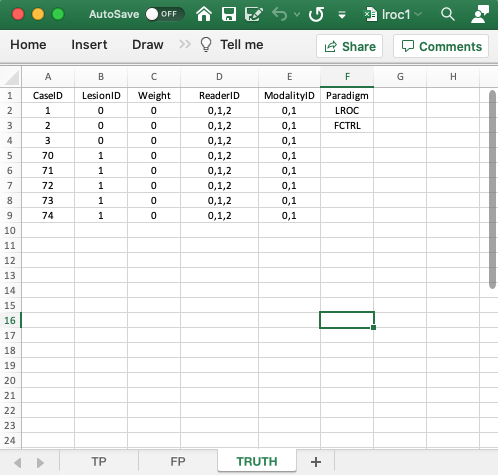
\includegraphics[width=1\textwidth,height=\textheight]{images/quick-start/lroc1Truth.png}

\begin{itemize}
\tightlist
\item
  The \texttt{Truth} worksheet is similar to that described previously for the ROC and LROC paradigms. The only difference is the first entry in the Paradigm column, which is \texttt{LROC}.
\item
  Since a diseased case has one lesion, the first five columns contain as many rows as there are cases in the dataset. There being 8 cases in the dataset, there are 8 rows of data.
\item
  \texttt{CaseID}: unique \textbf{integers} representing the cases in the dataset: `1', `2', `3', the 3 non-diseased cases, and `70', `71', `72', `73', `74', the 5 diseased cases.\\
\item
  \texttt{LesionID}: integers 0 or 1.

  \begin{itemize}
  \tightlist
  \item
    Each 0 represents a non-diseased case,
  \item
    Each 1 represents the solitary lesion in the diseased case.
  \end{itemize}
\item
  There are 3 non-diseased cases in the dataset (the number of 0's in the \texttt{LesionID} column).
\item
  There are 5 diseased cases in the dataset (the number of 1's in the \texttt{LesionID} column).
\item
  \texttt{Weight}: this column is filled with zeroes. With one lesion per case, the weights are irrelevant.
\item
  \texttt{ReaderID}: In the example shown each cell has the value `0, 1, 2'. There are 3 readers in the dataset, labeled \texttt{0}, \texttt{1} and \texttt{2}.
\item
  \texttt{ModalityID}: In the example each cell has the value \texttt{0,\ 1}. There are 2 modalities in the dataset, labeled \texttt{0} and \texttt{1}.
\item
  \texttt{Paradigm}: The contents are \texttt{LROC} and \texttt{FCTRL}: this is an \texttt{LROC} dataset and the design is ``factorial''.
\end{itemize}

\hypertarget{quick-start-lroc-tp1}{%
\section{\texorpdfstring{\texttt{TP} worksheet, forced localization true}{TP worksheet, forced localization true}}\label{quick-start-lroc-tp1}}

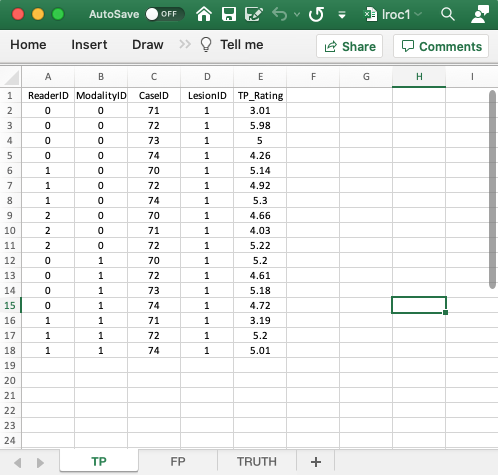
\includegraphics[width=1\textwidth,height=\textheight]{images/quick-start/lroc1TP.png}

\begin{itemize}
\tightlist
\item
  The \texttt{TP} worksheet is similar to that described previously for the ROC and FROC paradigms.
\item
  This worksheet can only have diseased cases. The presence of a non-diseased case in this worksheet will generate an error.
\item
  The key difference is that for each modality-reader and diseased-case combination there can be at most one entry. Also, if a particular combination is missing in the TP worksheet then it must appear in the FP worksheet. This is because this is a forced-mark-per-case dataset.
\item
  There can be at most 30 rows of data in this worksheet: 2 modalities times 3 readers times 5 diseased cases. Since there in fact only 17 rows of data, the missing 13 rows must occur in the FP worksheet.
\item
  Recall that each entry in the TP worksheet represents a correct localization while each missing entry represents an incorrect localization. The incorrect localizations are recorded in the FP worksheet.
\end{itemize}

\hypertarget{quick-start-lroc-fp1}{%
\section{\texorpdfstring{\texttt{FP} worksheet, forced localization true}{FP worksheet, forced localization true}}\label{quick-start-lroc-fp1}}

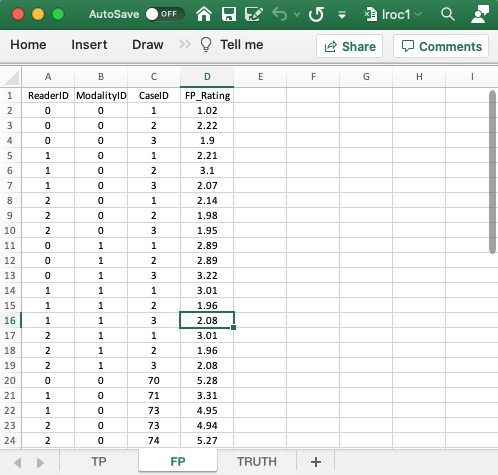
\includegraphics[width=1\textwidth,height=\textheight]{images/quick-start/lroc1FP1.png}

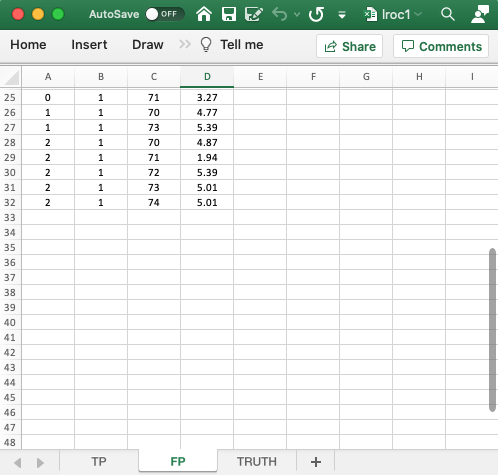
\includegraphics[width=1\textwidth,height=\textheight]{images/quick-start/lroc1FP2.png}

\begin{itemize}
\tightlist
\item
  The \texttt{FP} worksheet is similar to that described previously for the ROC and FROC paradigms.
\item
  Because of the forced mark requirement, there are 18 rows of data corresponding to non-diseased cases: 2 modalities times 3 readers times 3 non-diseased cases. The missing 13 rows from the TP worksheet are listed next; these correspond to the incorrect localizations on diseased cases. Therefore, the total number of rows in this worksheet is 18 + 13 = 31.
\item
  As an example, it is seen that for \texttt{modalityID} = 0 and \texttt{readerID} = 0, \texttt{caseID} = 70 does not appear in the TP worksheet. The lesion on this case was not localized; therefore it must appear in the FP worksheet as an incorrect localization, which is seen to be true in the FP worksheet.
\item
  As another example, for \texttt{modalityID} = 0 and \texttt{readerID} = 1, \texttt{caseID} = 71 does not appear in the TP worksheet; instead it appears in the FP worksheet.
\item
  As a final example, for \texttt{modalityID} = 1 and \texttt{readerID} = 2, none of the diseased cases appears in the TP worksheet; instead they all appear in the FP worksheet.
\end{itemize}

\hypertarget{quick-start-lroc-data-1}{%
\section{Reading forced localization true LROC dataset}\label{quick-start-lroc-data-1}}

The images shown above correspond to file \texttt{R/quick-start/lroc1.xlsx}. The next code reads this file into an \texttt{R} object \texttt{x1}. Note the usage of the \texttt{lrocForcedMark} flag, which is set to \texttt{TRUE}, because this is a forced localization LROC dataset.

\begin{Shaded}
\begin{Highlighting}[]
\NormalTok{lroc1 }\OtherTok{\textless{}{-}} \StringTok{"R/quick{-}start/lroc1.xlsx"}
\NormalTok{x1 }\OtherTok{\textless{}{-}} \FunctionTok{DfReadDataFile}\NormalTok{(lroc1, }\AttributeTok{newExcelFileFormat =} \ConstantTok{TRUE}\NormalTok{, }\AttributeTok{lrocForcedMark =}\NormalTok{ T)}
\FunctionTok{str}\NormalTok{(x1)}
\CommentTok{\#\textgreater{} List of 3}
\CommentTok{\#\textgreater{}  $ ratings     :List of 3}
\CommentTok{\#\textgreater{}   ..$ NL   : num [1:2, 1:3, 1:8, 1] 1.02 2.89 2.21 3.01 2.14 3.01 2.22 2.89 3.1 1.96 ...}
\CommentTok{\#\textgreater{}   ..$ LL   : num [1:2, 1:3, 1:5, 1] {-}Inf 5.2 5.14 {-}Inf 4.66 ...}
\CommentTok{\#\textgreater{}   ..$ LL\_IL: num [1:2, 1:3, 1:5, 1] 5.28 {-}Inf {-}Inf 4.77 {-}Inf ...}
\CommentTok{\#\textgreater{}  $ lesions     :List of 3}
\CommentTok{\#\textgreater{}   ..$ perCase: int [1:5] 1 1 1 1 1}
\CommentTok{\#\textgreater{}   ..$ IDs    : num [1:5, 1] 1 1 1 1 1}
\CommentTok{\#\textgreater{}   ..$ weights: num [1:5, 1] 1 1 1 1 1}
\CommentTok{\#\textgreater{}  $ descriptions:List of 7}
\CommentTok{\#\textgreater{}   ..$ fileName     : chr "lroc1"}
\CommentTok{\#\textgreater{}   ..$ type         : chr "LROC"}
\CommentTok{\#\textgreater{}   ..$ name         : logi NA}
\CommentTok{\#\textgreater{}   ..$ truthTableStr: num [1:2, 1:3, 1:8, 1:2] 1 1 1 1 1 1 1 1 1 1 ...}
\CommentTok{\#\textgreater{}   ..$ design       : chr "FCTRL"}
\CommentTok{\#\textgreater{}   ..$ modalityID   : Named chr [1:2] "0" "1"}
\CommentTok{\#\textgreater{}   .. ..{-} attr(*, "names")= chr [1:2] "0" "1"}
\CommentTok{\#\textgreater{}   ..$ readerID     : Named chr [1:3] "0" "1" "2"}
\CommentTok{\#\textgreater{}   .. ..{-} attr(*, "names")= chr [1:3] "0" "1" "2"}
\end{Highlighting}
\end{Shaded}

This follows the general description in Chapter \ref{quick-start-roc}. The differences are described below.

\begin{itemize}
\tightlist
\item
  \texttt{x1\$ratings\$NL} is a {[}2,3,8,1{]} dimension vector. For each modality and reader, only the first three elements, corresponding to the three non-diseased cases, are finite, the rest are \texttt{-Inf}.
\end{itemize}

For example:

\begin{Shaded}
\begin{Highlighting}[]
\NormalTok{x1}\SpecialCharTok{$}\NormalTok{ratings}\SpecialCharTok{$}\NormalTok{NL[}\DecValTok{1}\NormalTok{,}\DecValTok{1}\NormalTok{,,}\DecValTok{1}\NormalTok{]}
\CommentTok{\#\textgreater{} [1] 1.02 2.22 1.90 {-}Inf {-}Inf {-}Inf {-}Inf {-}Inf}
\end{Highlighting}
\end{Shaded}

\begin{itemize}
\tightlist
\item
  x1\(ratings\)LL\texttt{is\ a\ {[}2,3,5,1{]}\ dimension\ vector.\ For\ each\ modality\ and\ reader,\ only\ the\ first\ three\ elements,\ corresponding\ to\ the\ three\ non-diseased\ cases,\ are\ finite,\ the\ rest\ are}-Inf`.
\end{itemize}

For example, since none of the lesions are localized for \texttt{modalityID} = 1 (second modality) and \texttt{readerID} = 2 (third reader), the following code yields a vector consisting of five \texttt{-Inf} values:

\begin{Shaded}
\begin{Highlighting}[]
\NormalTok{x1}\SpecialCharTok{$}\NormalTok{ratings}\SpecialCharTok{$}\NormalTok{LL[}\DecValTok{2}\NormalTok{,}\DecValTok{3}\NormalTok{,,}\DecValTok{1}\NormalTok{]}
\CommentTok{\#\textgreater{} [1] {-}Inf {-}Inf {-}Inf {-}Inf {-}Inf}
\end{Highlighting}
\end{Shaded}

\begin{itemize}
\tightlist
\item
  \texttt{x1\$ratings\$LL\_IL} is a {[}2,3,5,1{]} dimension vector. These contain the ratings of incorrect localizations on diseased cases. For the just preceding modality-reader combination, this yields a vector with 5 finite values, the ratings of incorrect localizations for \texttt{modalityID} = 1 and \texttt{readerID} = 2.
\end{itemize}

\begin{Shaded}
\begin{Highlighting}[]
\NormalTok{x1}\SpecialCharTok{$}\NormalTok{ratings}\SpecialCharTok{$}\NormalTok{LL\_IL[}\DecValTok{2}\NormalTok{,}\DecValTok{3}\NormalTok{,,}\DecValTok{1}\NormalTok{]}
\CommentTok{\#\textgreater{} [1] 4.87 1.94 5.39 5.01 5.01}
\end{Highlighting}
\end{Shaded}

\hypertarget{quick-start-lroc-tp2}{%
\section{\texorpdfstring{\texttt{TP} worksheet, forced localization false}{TP worksheet, forced localization false}}\label{quick-start-lroc-tp2}}

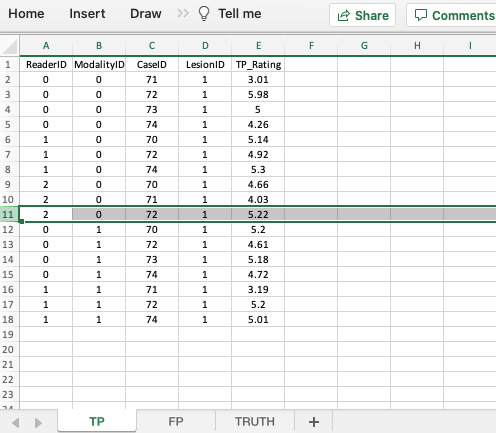
\includegraphics[width=1\textwidth,height=\textheight]{images/quick-start/lroc2TP.png}

\hypertarget{quick-start-lroc-fp2}{%
\section{\texorpdfstring{\texttt{FP} worksheet, forced localization false}{FP worksheet, forced localization false}}\label{quick-start-lroc-fp2}}

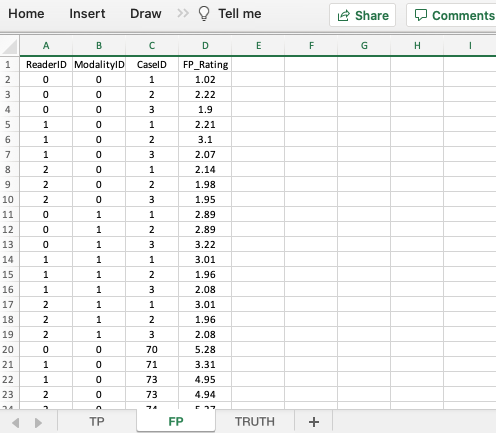
\includegraphics[width=1\textwidth,height=\textheight]{images/quick-start/lroc2FP1.png}

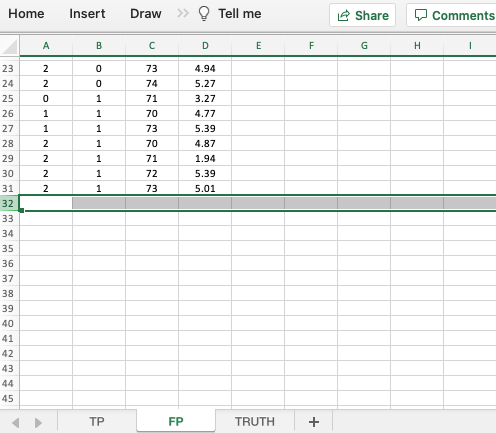
\includegraphics[width=1\textwidth,height=\textheight]{images/quick-start/lroc2FP2.png}

\begin{itemize}
\tightlist
\item
  If a particular modality-reader-case combination is missing in the TP worksheet then it need not appear in the FP worksheet. This is because this is not a forced-mark-per-case dataset.
\item
  As an example, \texttt{modalityID} = 1, \texttt{readerID} = 2 and \texttt{caseID} = 74 does not appear in either TP or FP worksheets.
\end{itemize}

\hypertarget{quick-start-lroc-data-2}{%
\section{Reading forced localization false LROC dataset}\label{quick-start-lroc-data-2}}

The next example is for file \texttt{R/quick-start/lroc2.xlsx}. The following code reads this file into an \texttt{R} object \texttt{x2}. Note that for this dataset one must set the \texttt{lrocForcedMark} flag to \texttt{FALSE}, because this is \emph{not} a forced localization LROC dataset. Setting \texttt{lrocForcedMark} flag to \texttt{TRUE} will generate an error.

\begin{Shaded}
\begin{Highlighting}[]
\NormalTok{lroc2 }\OtherTok{\textless{}{-}} \StringTok{"R/quick{-}start/lroc2.xlsx"}
\NormalTok{x2 }\OtherTok{\textless{}{-}} \FunctionTok{DfReadDataFile}\NormalTok{(lroc2, }\AttributeTok{newExcelFileFormat =} \ConstantTok{TRUE}\NormalTok{, }\AttributeTok{lrocForcedMark =}\NormalTok{ F)}
\FunctionTok{str}\NormalTok{(x2)}
\CommentTok{\#\textgreater{} List of 3}
\CommentTok{\#\textgreater{}  $ ratings     :List of 3}
\CommentTok{\#\textgreater{}   ..$ NL   : num [1:2, 1:3, 1:8, 1] 1.02 2.89 2.21 3.01 2.14 3.01 2.22 2.89 3.1 1.96 ...}
\CommentTok{\#\textgreater{}   ..$ LL   : num [1:2, 1:3, 1:5, 1] {-}Inf 5.2 5.14 {-}Inf 4.66 ...}
\CommentTok{\#\textgreater{}   ..$ LL\_IL: num [1:2, 1:3, 1:5, 1] 5.28 {-}Inf {-}Inf 4.77 {-}Inf ...}
\CommentTok{\#\textgreater{}  $ lesions     :List of 3}
\CommentTok{\#\textgreater{}   ..$ perCase: int [1:5] 1 1 1 1 1}
\CommentTok{\#\textgreater{}   ..$ IDs    : num [1:5, 1] 1 1 1 1 1}
\CommentTok{\#\textgreater{}   ..$ weights: num [1:5, 1] 1 1 1 1 1}
\CommentTok{\#\textgreater{}  $ descriptions:List of 7}
\CommentTok{\#\textgreater{}   ..$ fileName     : chr "lroc2"}
\CommentTok{\#\textgreater{}   ..$ type         : chr "LROC"}
\CommentTok{\#\textgreater{}   ..$ name         : logi NA}
\CommentTok{\#\textgreater{}   ..$ truthTableStr: num [1:2, 1:3, 1:8, 1:2] 1 1 1 1 1 1 1 1 1 1 ...}
\CommentTok{\#\textgreater{}   ..$ design       : chr "FCTRL"}
\CommentTok{\#\textgreater{}   ..$ modalityID   : Named chr [1:2] "0" "1"}
\CommentTok{\#\textgreater{}   .. ..{-} attr(*, "names")= chr [1:2] "0" "1"}
\CommentTok{\#\textgreater{}   ..$ readerID     : Named chr [1:3] "0" "1" "2"}
\CommentTok{\#\textgreater{}   .. ..{-} attr(*, "names")= chr [1:3] "0" "1" "2"}
\end{Highlighting}
\end{Shaded}

\begin{itemize}
\tightlist
\item
  The \texttt{x2\$ratings\$LL} array is a {[}2,3,5,1{]} dimension vector. For each modality and reader, only the first three elements, corresponding to the three non-diseased cases, are finite, the rest are \texttt{-Inf}.
\end{itemize}

For example, since none of the lesions are localized for \texttt{modalityID} = 1 (second modality) and \texttt{readerID} = 2 (third reader), the following code yields a vector consisting of five \texttt{-Inf} values:

\begin{Shaded}
\begin{Highlighting}[]
\NormalTok{x2}\SpecialCharTok{$}\NormalTok{ratings}\SpecialCharTok{$}\NormalTok{LL[}\DecValTok{2}\NormalTok{,}\DecValTok{3}\NormalTok{,,}\DecValTok{1}\NormalTok{]}
\CommentTok{\#\textgreater{} [1] {-}Inf {-}Inf {-}Inf {-}Inf {-}Inf}
\end{Highlighting}
\end{Shaded}

\begin{itemize}
\tightlist
\item
  The \texttt{x2\$ratings\$LL\_IL} is a {[}2,3,5,1{]} dimension vector. These contain the ratings of incorrect localizations on diseased cases. For the just preceding modality-reader combination, this yields a vector with 4 finite values, the ratings of incorrect localizations for \texttt{modalityID} = 1 and \texttt{readerID} = 2.
\end{itemize}

\begin{Shaded}
\begin{Highlighting}[]
\NormalTok{x2}\SpecialCharTok{$}\NormalTok{ratings}\SpecialCharTok{$}\NormalTok{LL\_IL[}\DecValTok{2}\NormalTok{,}\DecValTok{3}\NormalTok{,,}\DecValTok{1}\NormalTok{]}
\CommentTok{\#\textgreater{} [1] 4.87 1.94 5.39 5.01 {-}Inf}
\end{Highlighting}
\end{Shaded}

For this modality-reader combination case 74 (i.e., the fifth diseased case) was unmarked. It does not appear in either the TP or the FP worksheet.

\hypertarget{quick-start-lroc-data-summary}{%
\section{Summary}\label{quick-start-lroc-data-summary}}

The difference from the previous data structures is the existence of \texttt{LL\_IL} in the \texttt{ratings} list, which contains the ratings of incorrect localizations. Recall that for ROC and FROC paradigms this member was \texttt{NA}. When the data obeys forced localization, the corresponding flag should be set to \texttt{TRUE}, otherwise it should be set to \texttt{FALSE}. The default value of this flag is \texttt{NA}, which will work for ROC or FROC datasets. For LROC datasets it should be set to \texttt{T/F}.

\hypertarget{quick-start-dbm-text}{%
\chapter{DBM analysis text output}\label{quick-start-dbm-text}}

\hypertarget{quick-start-dbm-text-how-much-finished}{%
\section{TBA How much finished}\label{quick-start-dbm-text-how-much-finished}}

50\%

\hypertarget{quick-start-dbm-text-intro}{%
\section{Introduction}\label{quick-start-dbm-text-intro}}

This chapter illustrates significance testing using the DBM method.

\hypertarget{quick-start-dbm-text-analyze-dataset}{%
\section{Analyzing the ROC dataset}\label{quick-start-dbm-text-analyze-dataset}}

This illustrates the \texttt{StSignificanceTesting()} function. The significance testing method is specified as \texttt{"DBM"} and the figure of merit \texttt{FOM} is specified as ``Wilcoxon''. The embedded dataset \texttt{dataset03} is used.

\begin{Shaded}
\begin{Highlighting}[]
\NormalTok{ret }\OtherTok{\textless{}{-}} \FunctionTok{StSignificanceTesting}\NormalTok{(dataset03, }\AttributeTok{FOM =} \StringTok{"Wilcoxon"}\NormalTok{, }\AttributeTok{method =} \StringTok{"DBM"}\NormalTok{)}
\end{Highlighting}
\end{Shaded}

\hypertarget{quick-start-dbm-text-explanation}{%
\section{Explanation of the output}\label{quick-start-dbm-text-explanation}}

The function returns a list with 5 members:

\begin{itemize}
\tightlist
\item
  \texttt{FOMs}: figures of merit.
\item
  \texttt{ANOVA}: ANOVA tables.
\item
  \texttt{RRRC}: random-reader random-case analyses results.
\item
  \texttt{FRRC}: fixed-reader random-case analyses results.
\item
  \texttt{RRFC}'' random-reader fixed-case analyses results.
\end{itemize}

Let us consider them individually.

\begin{Shaded}
\begin{Highlighting}[]
\FunctionTok{str}\NormalTok{(ret}\SpecialCharTok{$}\NormalTok{FOMs)}
\CommentTok{\#\textgreater{} List of 3}
\CommentTok{\#\textgreater{}  $ foms        :\textquotesingle{}data.frame\textquotesingle{}:    2 obs. of  4 variables:}
\CommentTok{\#\textgreater{}   ..$ rdrREADER\_1: num [1:2] 0.853 0.85}
\CommentTok{\#\textgreater{}   ..$ rdrREADER\_2: num [1:2] 0.865 0.844}
\CommentTok{\#\textgreater{}   ..$ rdrREADER\_3: num [1:2] 0.857 0.84}
\CommentTok{\#\textgreater{}   ..$ rdrREADER\_4: num [1:2] 0.815 0.814}
\CommentTok{\#\textgreater{}  $ trtMeans    :\textquotesingle{}data.frame\textquotesingle{}:    2 obs. of  1 variable:}
\CommentTok{\#\textgreater{}   ..$ Estimate: num [1:2] 0.848 0.837}
\CommentTok{\#\textgreater{}  $ trtMeanDiffs:\textquotesingle{}data.frame\textquotesingle{}:    1 obs. of  1 variable:}
\CommentTok{\#\textgreater{}   ..$ Estimate: num 0.0109}
\end{Highlighting}
\end{Shaded}

\begin{itemize}
\tightlist
\item
  \texttt{FOMs} is a list of 3

  \begin{itemize}
  \tightlist
  \item
    \texttt{foms} is a {[}2x4{]} dataframe: the figure of merit for each of of the four observers in the two treatments.
  \item
    \texttt{trtMeans} is a {[}2x1{]} dataframe: the average figure of merit over all readers for each treatment.
  \item
    \texttt{trtMeanDiffs} a {[}1x1{]} dataframe: the difference(s) of the reader-averaged figures of merit for all different-treatment pairings. In this example, with only two treatments, there is only one different-treatment pairing.
  \end{itemize}
\end{itemize}

\begin{Shaded}
\begin{Highlighting}[]
\NormalTok{ret}\SpecialCharTok{$}\NormalTok{FOMs}\SpecialCharTok{$}\NormalTok{foms}
\CommentTok{\#\textgreater{}           rdrREADER\_1 rdrREADER\_2 rdrREADER\_3 rdrREADER\_4}
\CommentTok{\#\textgreater{} trtTREAT1  0.85345997  0.86499322  0.85730439  0.81524197}
\CommentTok{\#\textgreater{} trtTREAT2  0.84961556  0.84350972  0.84011759  0.81433740}
\NormalTok{ret}\SpecialCharTok{$}\NormalTok{FOMs}\SpecialCharTok{$}\NormalTok{trtMeans}
\CommentTok{\#\textgreater{}             Estimate}
\CommentTok{\#\textgreater{} trtTREAT1 0.84774989}
\CommentTok{\#\textgreater{} trtTREAT2 0.83689507}
\NormalTok{ret}\SpecialCharTok{$}\NormalTok{FOMs}\SpecialCharTok{$}\NormalTok{trtMeanDiffs}
\CommentTok{\#\textgreater{}                        Estimate}
\CommentTok{\#\textgreater{} trtTREAT1{-}trtTREAT2 0.010854817}
\end{Highlighting}
\end{Shaded}

\begin{Shaded}
\begin{Highlighting}[]
\FunctionTok{str}\NormalTok{(ret}\SpecialCharTok{$}\NormalTok{ANOVA)}
\CommentTok{\#\textgreater{} List of 4}
\CommentTok{\#\textgreater{}  $ TRCanova     :\textquotesingle{}data.frame\textquotesingle{}:   8 obs. of  3 variables:}
\CommentTok{\#\textgreater{}   ..$ SS: num [1:8] 0.0236 0.2052 52.5284 0.0151 6.41 ...}
\CommentTok{\#\textgreater{}   ..$ DF: num [1:8] 1 3 99 3 99 297 297 799}
\CommentTok{\#\textgreater{}   ..$ MS: num [1:8] 0.02357 0.06841 0.53059 0.00502 0.06475 ...}
\CommentTok{\#\textgreater{}  $ VarCom       :\textquotesingle{}data.frame\textquotesingle{}:   6 obs. of  1 variable:}
\CommentTok{\#\textgreater{}   ..$ Estimates: num [1:6] 3.78e{-}05 5.13e{-}02 {-}7.13e{-}04 {-}2.89e{-}03 2.79e{-}02 ...}
\CommentTok{\#\textgreater{}  $ IndividualTrt:\textquotesingle{}data.frame\textquotesingle{}:   3 obs. of  3 variables:}
\CommentTok{\#\textgreater{}   ..$ DF       : num [1:3] 3 99 297}
\CommentTok{\#\textgreater{}   ..$ TrtTREAT1: num [1:3] 0.0493 0.294 0.105}
\CommentTok{\#\textgreater{}   ..$ TrtTREAT2: num [1:3] 0.0242 0.3014 0.1034}
\CommentTok{\#\textgreater{}  $ IndividualRdr:\textquotesingle{}data.frame\textquotesingle{}:   3 obs. of  5 variables:}
\CommentTok{\#\textgreater{}   ..$ DF         : num [1:3] 1 99 99}
\CommentTok{\#\textgreater{}   ..$ rdrREADER\_1: num [1:3] 0.000739 0.203875 0.091559}
\CommentTok{\#\textgreater{}   ..$ rdrREADER\_2: num [1:3] 0.0231 0.2234 0.0803}
\CommentTok{\#\textgreater{}   ..$ rdrREADER\_3: num [1:3] 0.0148 0.2142 0.0612}
\CommentTok{\#\textgreater{}   ..$ rdrREADER\_4: num [1:3] 4.09e{-}05 2.85e{-}01 6.06e{-}02}
\end{Highlighting}
\end{Shaded}

\begin{itemize}
\tightlist
\item
  ANOVA is a list of 4

  \begin{itemize}
  \tightlist
  \item
    \texttt{TRCanova} is a {[}8x3{]} dataframe: the treatment-reader-case ANOVA table, see below, where SS is the sum of squares, DF is the denominator degrees of freedom and MS is the mean squares, and T = treatment, R = reader, C = case, TR = treatment-reader, TC = treatment-case, RC = reader-case, TRC = treatment-reader-case.\\
  \item
    \texttt{VarCom} is a {[}6x1{]} dataframe: the variance components, see below, where \texttt{varR} is the reader variance, \texttt{varC} is the case variance, \texttt{varTR} is the treatment-reader variance, \texttt{varTC} is the treatment-case variance, \texttt{varRC} is the reader-case variance, and \texttt{varTRC} is the treatment-reader-case variance.
  \item
    \texttt{IndividualTrt} is a {[}3x3{]} dataframe: the individual treatment variance components averaged over all readers, see below, where \texttt{msR} is the mean square reader, \texttt{msC} is the mean square case and \texttt{msRC} is the mean square reader-case.
  \item
    \texttt{IndividualRdr} is a {[}3x5{]} dataframe: the individual reader variance components averaged over treatments, see below, where \texttt{msT} is the mean square treatment, \texttt{msC} is the mean square case and \texttt{msTC} is the mean square treatment-case.
  \end{itemize}
\end{itemize}

\begin{Shaded}
\begin{Highlighting}[]
\NormalTok{ret}\SpecialCharTok{$}\NormalTok{ANOVA}\SpecialCharTok{$}\NormalTok{TRCanova}
\CommentTok{\#\textgreater{}                  SS  DF           MS}
\CommentTok{\#\textgreater{} T       0.023565410   1 0.0235654097}
\CommentTok{\#\textgreater{} R       0.205217999   3 0.0684059998}
\CommentTok{\#\textgreater{} C      52.528398680  99 0.5305898857}
\CommentTok{\#\textgreater{} TR      0.015060792   3 0.0050202641}
\CommentTok{\#\textgreater{} TC      6.410048814  99 0.0647479678}
\CommentTok{\#\textgreater{} RC     39.242953812 297 0.1321311576}
\CommentTok{\#\textgreater{} TRC    22.660077641 297 0.0762965577}
\CommentTok{\#\textgreater{} Total 121.085323149 799           NA}
\NormalTok{ret}\SpecialCharTok{$}\NormalTok{ANOVA}\SpecialCharTok{$}\NormalTok{VarCom}
\CommentTok{\#\textgreater{}             Estimates}
\CommentTok{\#\textgreater{} VarR    3.7755679e{-}05}
\CommentTok{\#\textgreater{} VarC    5.1250915e{-}02}
\CommentTok{\#\textgreater{} VarTR  {-}7.1276294e{-}04}
\CommentTok{\#\textgreater{} VarTC  {-}2.8871475e{-}03}
\CommentTok{\#\textgreater{} VarRC   2.7917300e{-}02}
\CommentTok{\#\textgreater{} VarErr  7.6296558e{-}02}
\NormalTok{ret}\SpecialCharTok{$}\NormalTok{ANOVA}\SpecialCharTok{$}\NormalTok{IndividualTrt}
\CommentTok{\#\textgreater{}       DF   TrtTREAT1   TrtTREAT2}
\CommentTok{\#\textgreater{} msR    3 0.049266349 0.024159915}
\CommentTok{\#\textgreater{} msC   99 0.293967531 0.301370323}
\CommentTok{\#\textgreater{} msRC 297 0.105047872 0.103379843}
\NormalTok{ret}\SpecialCharTok{$}\NormalTok{ANOVA}\SpecialCharTok{$}\NormalTok{IndividualRdr}
\CommentTok{\#\textgreater{}      DF   rdrREADER\_1 rdrREADER\_2 rdrREADER\_3   rdrREADER\_4}
\CommentTok{\#\textgreater{} msT   1 0.00073897606 0.023077021 0.014769293 0.00004091217}
\CommentTok{\#\textgreater{} msC  99 0.20387477465 0.223441908 0.214246773 0.28541990211}
\CommentTok{\#\textgreater{} msTC 99 0.09155873437 0.080279256 0.061228980 0.06057067104}
\end{Highlighting}
\end{Shaded}

\begin{Shaded}
\begin{Highlighting}[]
\FunctionTok{str}\NormalTok{(ret}\SpecialCharTok{$}\NormalTok{RRRC)}
\CommentTok{\#\textgreater{} List of 3}
\CommentTok{\#\textgreater{}  $ FTests         :\textquotesingle{}data.frame\textquotesingle{}: 2 obs. of  4 variables:}
\CommentTok{\#\textgreater{}   ..$ DF   : num [1:2] 1 3}
\CommentTok{\#\textgreater{}   ..$ MS   : num [1:2] 0.02357 0.00502}
\CommentTok{\#\textgreater{}   ..$ FStat: num [1:2] 4.69 NA}
\CommentTok{\#\textgreater{}   ..$ p    : num [1:2] 0.119 NA}
\CommentTok{\#\textgreater{}  $ ciDiffTrt      :\textquotesingle{}data.frame\textquotesingle{}: 1 obs. of  7 variables:}
\CommentTok{\#\textgreater{}   ..$ Estimate: num 0.0109}
\CommentTok{\#\textgreater{}   ..$ StdErr  : num 0.00501}
\CommentTok{\#\textgreater{}   ..$ DF      : num 3}
\CommentTok{\#\textgreater{}   ..$ t       : num 2.17}
\CommentTok{\#\textgreater{}   ..$ PrGTt   : num 0.119}
\CommentTok{\#\textgreater{}   ..$ CILower : num {-}0.00509}
\CommentTok{\#\textgreater{}   ..$ CIUpper : num 0.0268}
\CommentTok{\#\textgreater{}  $ ciAvgRdrEachTrt:\textquotesingle{}data.frame\textquotesingle{}: 2 obs. of  5 variables:}
\CommentTok{\#\textgreater{}   ..$ Estimate: num [1:2] 0.848 0.837}
\CommentTok{\#\textgreater{}   ..$ StdErr  : num [1:2] 0.0244 0.0236}
\CommentTok{\#\textgreater{}   ..$ DF      : num [1:2] 70.1 253.6}
\CommentTok{\#\textgreater{}   ..$ CILower : num [1:2] 0.799 0.79}
\CommentTok{\#\textgreater{}   ..$ CIUpper : num [1:2] 0.896 0.883}
\end{Highlighting}
\end{Shaded}

\begin{itemize}
\tightlist
\item
  RRRC, a list of 3 containing results of random-reader random-case analyses

  \begin{itemize}
  \tightlist
  \item
    \texttt{FTtests}: is a {[}2x4{]} dataframe: results of the F-tests, see below, where \texttt{FStat} is the F-statistic and \texttt{p} is the p-value. The first row is the treatment effect and the second is the error term.
  \item
    \texttt{ciDiffTrt}: is a {[}1x7{]} dataframe: the confidence intervals between different-treatments, see below, where \texttt{StdErr} is the standard error of the estimate, \texttt{t} is the t-statistic and \texttt{PrGTt} is the p-value.
  \item
    \texttt{ciAvgRdrEachTrt}: is a {[}2x5{]} dataframe: the confidence intervals for each treatment, averaged over all readers in the treatment, see below, where \texttt{CILower} is the lower 95\% confidence interval and \texttt{CIUpper} is the upper 95\% confidence interval.
  \end{itemize}
\end{itemize}

\begin{Shaded}
\begin{Highlighting}[]
\NormalTok{ret}\SpecialCharTok{$}\NormalTok{RRRC}\SpecialCharTok{$}\NormalTok{FTests}
\CommentTok{\#\textgreater{}           DF           MS     FStat          p}
\CommentTok{\#\textgreater{} Treatment  1 0.0235654097 4.6940577 0.11883786}
\CommentTok{\#\textgreater{} Error      3 0.0050202641        NA         NA}
\NormalTok{ret}\SpecialCharTok{$}\NormalTok{RRRC}\SpecialCharTok{$}\NormalTok{ciDiffTrt}
\CommentTok{\#\textgreater{}                        Estimate       StdErr DF         t      PrGTt}
\CommentTok{\#\textgreater{} trtTREAT1{-}trtTREAT2 0.010854817 0.0050101218  3 2.1665774 0.11883786}
\CommentTok{\#\textgreater{}                           CILower     CIUpper}
\CommentTok{\#\textgreater{} trtTREAT1{-}trtTREAT2 {-}0.0050896269 0.026799261}
\NormalTok{ret}\SpecialCharTok{$}\NormalTok{RRRC}\SpecialCharTok{$}\NormalTok{ciAvgRdrEachTrt}
\CommentTok{\#\textgreater{}             Estimate      StdErr         DF    CILower    CIUpper}
\CommentTok{\#\textgreater{} trtTREAT1 0.84774989 0.024402152  70.121788 0.79908282 0.89641696}
\CommentTok{\#\textgreater{} trtTREAT2 0.83689507 0.023566416 253.644028 0.79048429 0.88330585}
\end{Highlighting}
\end{Shaded}

\begin{Shaded}
\begin{Highlighting}[]
\FunctionTok{str}\NormalTok{(ret}\SpecialCharTok{$}\NormalTok{FRRC)}
\CommentTok{\#\textgreater{} List of 4}
\CommentTok{\#\textgreater{}  $ FTests          :\textquotesingle{}data.frame\textquotesingle{}:    2 obs. of  4 variables:}
\CommentTok{\#\textgreater{}   ..$ DF   : num [1:2] 1 99}
\CommentTok{\#\textgreater{}   ..$ MS   : num [1:2] 0.0236 0.0647}
\CommentTok{\#\textgreater{}   ..$ FStat: num [1:2] 0.364 NA}
\CommentTok{\#\textgreater{}   ..$ p    : num [1:2] 0.548 NA}
\CommentTok{\#\textgreater{}  $ ciDiffTrt       :\textquotesingle{}data.frame\textquotesingle{}:    1 obs. of  7 variables:}
\CommentTok{\#\textgreater{}   ..$ Estimate: num 0.0109}
\CommentTok{\#\textgreater{}   ..$ StdErr  : num 0.018}
\CommentTok{\#\textgreater{}   ..$ DF      : num 99}
\CommentTok{\#\textgreater{}   ..$ t       : num 0.603}
\CommentTok{\#\textgreater{}   ..$ PrGTt   : num 0.548}
\CommentTok{\#\textgreater{}   ..$ CILower : num {-}0.0248}
\CommentTok{\#\textgreater{}   ..$ CIUpper : num 0.0466}
\CommentTok{\#\textgreater{}  $ ciAvgRdrEachTrt :\textquotesingle{}data.frame\textquotesingle{}:    2 obs. of  5 variables:}
\CommentTok{\#\textgreater{}   ..$ Estimate: num [1:2] 0.848 0.837}
\CommentTok{\#\textgreater{}   ..$ StdErr  : num [1:2] 0.0271 0.0274}
\CommentTok{\#\textgreater{}   ..$ DF      : num [1:2] 99 99}
\CommentTok{\#\textgreater{}   ..$ CILower : num [1:2] 0.794 0.782}
\CommentTok{\#\textgreater{}   ..$ CIUpper : num [1:2] 0.902 0.891}
\CommentTok{\#\textgreater{}  $ ciDiffTrtEachRdr:\textquotesingle{}data.frame\textquotesingle{}:    4 obs. of  7 variables:}
\CommentTok{\#\textgreater{}   ..$ Estimate: num [1:4] 0.003844 0.021483 0.017187 0.000905}
\CommentTok{\#\textgreater{}   ..$ StdErr  : num [1:4] 0.0428 0.0401 0.035 0.0348}
\CommentTok{\#\textgreater{}   ..$ DF      : num [1:4] 99 99 99 99}
\CommentTok{\#\textgreater{}   ..$ t       : num [1:4] 0.0898 0.5362 0.4911 0.026}
\CommentTok{\#\textgreater{}   ..$ PrGTt   : num [1:4] 0.929 0.593 0.624 0.979}
\CommentTok{\#\textgreater{}   ..$ CILower : num [1:4] {-}0.0811 {-}0.058 {-}0.0522 {-}0.0682}
\CommentTok{\#\textgreater{}   ..$ CIUpper : num [1:4] 0.0888 0.101 0.0866 0.07}
\end{Highlighting}
\end{Shaded}

\begin{itemize}
\tightlist
\item
  FRRC, a list of 4 containing results of fixed-reader random-case analyses

  \begin{itemize}
  \tightlist
  \item
    \texttt{FTtests}: is a {[}2x4{]} dataframe: results of the F-tests, see below.
  \item
    \texttt{ciDiffTrt}: is a {[}1x7{]} dataframe: the confidence intervals between different-treatments, see below.
  \item
    \texttt{ciAvgRdrEachTrt}: is a {[}2x5{]} dataframe: the confidence intervals for the average reader over each treatment
  \item
    \texttt{ciDiffTrtEachRdr}: is a {[}4x7{]} dataframe: the confidence intervals for each different-treatment pairing for each reader.
  \end{itemize}
\end{itemize}

\begin{Shaded}
\begin{Highlighting}[]
\NormalTok{ret}\SpecialCharTok{$}\NormalTok{FRRC}\SpecialCharTok{$}\NormalTok{FTests}
\CommentTok{\#\textgreater{}           DF          MS      FStat          p}
\CommentTok{\#\textgreater{} Treatment  1 0.023565410 0.36395597 0.54769704}
\CommentTok{\#\textgreater{} Error     99 0.064747968         NA         NA}
\NormalTok{ret}\SpecialCharTok{$}\NormalTok{FRRC}\SpecialCharTok{$}\NormalTok{ciDiffTrt}
\CommentTok{\#\textgreater{}                        Estimate      StdErr DF          t      PrGTt}
\CommentTok{\#\textgreater{} trtTREAT1{-}trtTREAT2 0.010854817 0.017992772 99 0.60328764 0.54769704}
\CommentTok{\#\textgreater{}                          CILower    CIUpper}
\CommentTok{\#\textgreater{} trtTREAT1{-}trtTREAT2 {-}0.024846746 0.04655638}
\NormalTok{ret}\SpecialCharTok{$}\NormalTok{FRRC}\SpecialCharTok{$}\NormalTok{ciAvgRdrEachTrt}
\CommentTok{\#\textgreater{}             Estimate      StdErr DF    CILower    CIUpper}
\CommentTok{\#\textgreater{} trtTREAT1 0.84774989 0.027109386 99 0.79395898 0.90154079}
\CommentTok{\#\textgreater{} trtTREAT2 0.83689507 0.027448603 99 0.78243109 0.89135905}
\NormalTok{ret}\SpecialCharTok{$}\NormalTok{FRRC}\SpecialCharTok{$}\NormalTok{ciDiffTrtEachRdr}
\CommentTok{\#\textgreater{}                                       Estimate      StdErr DF           t}
\CommentTok{\#\textgreater{} rdrREADER\_1::trtTREAT1{-}trtTREAT2 0.00384441429 0.042792227 99 0.089839080}
\CommentTok{\#\textgreater{} rdrREADER\_2::trtTREAT1{-}trtTREAT2 0.02148349163 0.040069753 99 0.536152334}
\CommentTok{\#\textgreater{} rdrREADER\_3::trtTREAT1{-}trtTREAT2 0.01718679331 0.034993994 99 0.491135520}
\CommentTok{\#\textgreater{} rdrREADER\_4::trtTREAT1{-}trtTREAT2 0.00090456807 0.034805365 99 0.025989329}
\CommentTok{\#\textgreater{}                                       PrGTt      CILower     CIUpper}
\CommentTok{\#\textgreater{} rdrREADER\_1::trtTREAT1{-}trtTREAT2 0.92859660 {-}0.081064648 0.088753476}
\CommentTok{\#\textgreater{} rdrREADER\_2::trtTREAT1{-}trtTREAT2 0.59305592 {-}0.058023592 0.100990575}
\CommentTok{\#\textgreater{} rdrREADER\_3::trtTREAT1{-}trtTREAT2 0.62441761 {-}0.052248882 0.086622469}
\CommentTok{\#\textgreater{} rdrREADER\_4::trtTREAT1{-}trtTREAT2 0.97931817 {-}0.068156827 0.069965963}
\end{Highlighting}
\end{Shaded}

\begin{Shaded}
\begin{Highlighting}[]
\FunctionTok{str}\NormalTok{(ret}\SpecialCharTok{$}\NormalTok{RRFC)}
\CommentTok{\#\textgreater{} List of 3}
\CommentTok{\#\textgreater{}  $ FTests         :\textquotesingle{}data.frame\textquotesingle{}: 2 obs. of  4 variables:}
\CommentTok{\#\textgreater{}   ..$ DF   : num [1:2] 1 3}
\CommentTok{\#\textgreater{}   ..$ MS   : num [1:2] 0.02357 0.00502}
\CommentTok{\#\textgreater{}   ..$ FStat: num [1:2] 4.69 NA}
\CommentTok{\#\textgreater{}   ..$ p    : num [1:2] 0.119 NA}
\CommentTok{\#\textgreater{}  $ ciDiffTrt      :\textquotesingle{}data.frame\textquotesingle{}: 1 obs. of  7 variables:}
\CommentTok{\#\textgreater{}   ..$ Estimate: num 0.0109}
\CommentTok{\#\textgreater{}   ..$ StdErr  : num 0.00501}
\CommentTok{\#\textgreater{}   ..$ DF      : num 3}
\CommentTok{\#\textgreater{}   ..$ t       : num 2.17}
\CommentTok{\#\textgreater{}   ..$ PrGTt   : num 0.119}
\CommentTok{\#\textgreater{}   ..$ CILower : num {-}0.00509}
\CommentTok{\#\textgreater{}   ..$ CIUpper : num 0.0268}
\CommentTok{\#\textgreater{}  $ ciAvgRdrEachTrt:\textquotesingle{}data.frame\textquotesingle{}: 2 obs. of  5 variables:}
\CommentTok{\#\textgreater{}   ..$ Estimate: num [1:2] 0.848 0.837}
\CommentTok{\#\textgreater{}   ..$ StdErr  : num [1:2] 0.0111 0.00777}
\CommentTok{\#\textgreater{}   ..$ DF      : num [1:2] 3 3}
\CommentTok{\#\textgreater{}   ..$ CILower : num [1:2] 0.812 0.812}
\CommentTok{\#\textgreater{}   ..$ CIUpper : num [1:2] 0.883 0.862}
\end{Highlighting}
\end{Shaded}

\begin{itemize}
\tightlist
\item
  RRFC, a list of 3 containing results of random-reader fixed-case analyses

  \begin{itemize}
  \tightlist
  \item
    \texttt{FTtests}: is a {[}2x4{]} dataframe: results of the F-tests, see below.
  \item
    \texttt{ciDiffTrt}: is a {[}1x7{]} dataframe: the confidence intervals between different-treatments, see below.
  \item
    \texttt{ciAvgRdrEachTrt}: is a {[}2x5{]} dataframe: the confidence intervals for the average reader over each over each treatment.
  \end{itemize}
\end{itemize}

\begin{Shaded}
\begin{Highlighting}[]
\NormalTok{ret}\SpecialCharTok{$}\NormalTok{RRFC}\SpecialCharTok{$}\NormalTok{FTests}
\CommentTok{\#\textgreater{}           DF           MS     FStat          p}
\CommentTok{\#\textgreater{} Treatment  1 0.0235654097 4.6940577 0.11883786}
\CommentTok{\#\textgreater{} Error      3 0.0050202641        NA         NA}
\NormalTok{ret}\SpecialCharTok{$}\NormalTok{RRFC}\SpecialCharTok{$}\NormalTok{ciDiffTrt}
\CommentTok{\#\textgreater{}                        Estimate       StdErr DF         t      PrGTt}
\CommentTok{\#\textgreater{} trtTREAT1{-}trtTREAT2 0.010854817 0.0050101218  3 2.1665774 0.11883786}
\CommentTok{\#\textgreater{}                           CILower     CIUpper}
\CommentTok{\#\textgreater{} trtTREAT1{-}trtTREAT2 {-}0.0050896269 0.026799261}
\NormalTok{ret}\SpecialCharTok{$}\NormalTok{RRFC}\SpecialCharTok{$}\NormalTok{ciAvgRdrEachTrt}
\CommentTok{\#\textgreater{}             Estimate      StdErr DF    CILower    CIUpper}
\CommentTok{\#\textgreater{} trtTREAT1 0.84774989 0.011098012  3 0.81243106 0.88306871}
\CommentTok{\#\textgreater{} trtTREAT2 0.83689507 0.007771730  3 0.81216196 0.86162818}
\end{Highlighting}
\end{Shaded}

\hypertarget{quick-start-or-text}{%
\chapter{OR analysis text output}\label{quick-start-or-text}}

\hypertarget{quick-start-or-text-how-much-finished}{%
\section{TBA How much finished}\label{quick-start-or-text-how-much-finished}}

90\%

\hypertarget{quick-start-or-text-intro}{%
\section{Introduction}\label{quick-start-or-text-intro}}

This chapter illustrates significance testing using the DBM and OR methods.

\hypertarget{quick-start-or-text-analyze-dataset}{%
\section{Analyzing the ROC dataset}\label{quick-start-or-text-analyze-dataset}}

The only change is to specify \texttt{method\ =\ "OR"} in the significance testing function. The same dataset is used as was used in the previous chapter.

\begin{Shaded}
\begin{Highlighting}[]
\NormalTok{ret }\OtherTok{\textless{}{-}} \FunctionTok{StSignificanceTesting}\NormalTok{(dataset03, }\AttributeTok{FOM =} \StringTok{"Wilcoxon"}\NormalTok{, }\AttributeTok{method =} \StringTok{"OR"}\NormalTok{)}
\end{Highlighting}
\end{Shaded}

\hypertarget{quick-start-or-text-explanation}{%
\section{Explanation of the output}\label{quick-start-or-text-explanation}}

The function returns a list with 5 members.

\begin{itemize}
\tightlist
\item
  \texttt{FOMs}: figures of merit, identical to that in the DBM method.
\item
  \texttt{ANOVA}: ANOVA tables.
\item
  \texttt{RRRC}: random-reader random-case analyses results.
\item
  \texttt{FRRC}: fixed-reader random-case analyses results.
\item
  \texttt{RRFC}'' random-reader fixed-case analyses results.
\end{itemize}

Let us consider the ones that are different from the DBM method.

\begin{itemize}
\tightlist
\item
  ANOVA is a list of 4

  \begin{itemize}
  \tightlist
  \item
    \texttt{TRanova} is a {[}3x3{]} dataframe: the treatment-reader ANOVA table, see below, where SS is the sum of squares, DF is the denominator degrees of freedom and MS is the mean squares, and T = treatment, R = reader, TR = treatment-reader.\\
  \item
    \texttt{VarCom} is a {[}6x2{]} dataframe: the variance components, see below, where \texttt{varR} is the reader variance, \texttt{varTR} is the treatment-reader variance, \texttt{Cov1}, \texttt{Cov2},\texttt{Cov3} and \texttt{Var} are as defined in the OR model. The second column lists the correlations defined in the OR model.
  \item
    \texttt{IndividualTrt} is a {[}2x4{]} dataframe: the individual treatment mean-squares, variances and \(Cov_2\), averaged over all readers, see below, where \texttt{msREachTrt} is the mean square reader, \texttt{varEachTrt} is the variance and \texttt{cov2EachTrt} is \texttt{Cov2EachTrt} in each treatment.
  \item
    \texttt{IndividualRdr} is a {[}2x4{]} dataframe: the individual reader variance components averaged over treatments, see below, where \texttt{msTEachRdr} is the mean square treatment, \texttt{varEachRdr} is the variance and \texttt{cov1EachRdr} is \(Cov_1\) for each reader.
  \end{itemize}
\end{itemize}

\begin{Shaded}
\begin{Highlighting}[]
\NormalTok{ret}\SpecialCharTok{$}\NormalTok{ANOVA}\SpecialCharTok{$}\NormalTok{TRanova}
\CommentTok{\#\textgreater{}               SS DF            MS}
\CommentTok{\#\textgreater{} T  0.00023565410  1 2.3565410e{-}04}
\CommentTok{\#\textgreater{} R  0.00205217999  3 6.8406000e{-}04}
\CommentTok{\#\textgreater{} TR 0.00015060792  3 5.0202641e{-}05}
\NormalTok{ret}\SpecialCharTok{$}\NormalTok{ANOVA}\SpecialCharTok{$}\NormalTok{VarCom}
\CommentTok{\#\textgreater{}            Estimates       Rhos}
\CommentTok{\#\textgreater{} VarR   2.3319942e{-}05         NA}
\CommentTok{\#\textgreater{} VarTR {-}6.8389146e{-}04         NA}
\CommentTok{\#\textgreater{} Cov1   7.9168215e{-}04 0.51887172}
\CommentTok{\#\textgreater{} Cov2   4.8363767e{-}04 0.31697811}
\CommentTok{\#\textgreater{} Cov3   5.1250915e{-}04 0.33590059}
\CommentTok{\#\textgreater{} Var    1.5257762e{-}03         NA}
\NormalTok{ret}\SpecialCharTok{$}\NormalTok{ANOVA}\SpecialCharTok{$}\NormalTok{IndividualTrt}
\CommentTok{\#\textgreater{}           DF    msREachTrt   varEachTrt   cov2EachTrt}
\CommentTok{\#\textgreater{} trtTREAT1  3 0.00049266349 0.0015227779 0.00047229915}
\CommentTok{\#\textgreater{} trtTREAT2  3 0.00024159915 0.0015287746 0.00049497620}
\NormalTok{ret}\SpecialCharTok{$}\NormalTok{ANOVA}\SpecialCharTok{$}\NormalTok{IndividualRdr}
\CommentTok{\#\textgreater{}             DF    msTEachRdr   varEachRdr   cov1EachRdr}
\CommentTok{\#\textgreater{} rdrREADER\_1  1 7.3897606e{-}06 0.0014771675 0.00056158020}
\CommentTok{\#\textgreater{} rdrREADER\_2  1 2.3077021e{-}04 0.0015186058 0.00071581326}
\CommentTok{\#\textgreater{} rdrREADER\_3  1 1.4769293e{-}04 0.0013773788 0.00076508897}
\CommentTok{\#\textgreater{} rdrREADER\_4  1 4.0912170e{-}07 0.0017299529 0.00112424616}
\end{Highlighting}
\end{Shaded}

\begin{itemize}
\tightlist
\item
  RRRC, a list of 3 containing results of random-reader random-case analyses

  \begin{itemize}
  \tightlist
  \item
    \texttt{FTtests}: is a {[}2x4{]} dataframe: results of the F-tests, see below, where \texttt{FStat} is the F-statistic and \texttt{p} is the p-value. The first row is the treatment effect and the second is the error term.
  \item
    \texttt{ciDiffTrt}: is a {[}1x7{]} dataframe: the confidence intervals between different treatments, see below, where \texttt{StdErr} is the standard error of the estimate, \texttt{t} is the t-statistic and \texttt{PrGTt} is the p-value.
  \item
    \texttt{ciAvgRdrEachTrt}: is a {[}2x5{]} dataframe: the confidence intervals for the average reader over each treatment, see below, where \texttt{CILower} is the lower 95\% confidence interval and \texttt{CIUpper} is the upper 95\% confidence interval.
  \end{itemize}
\end{itemize}

\begin{Shaded}
\begin{Highlighting}[]
\NormalTok{ret}\SpecialCharTok{$}\NormalTok{RRRC}\SpecialCharTok{$}\NormalTok{FTests}
\CommentTok{\#\textgreater{}           DF            MS     FStat          p}
\CommentTok{\#\textgreater{} Treatment  1 2.3565410e{-}04 4.6940577 0.11883786}
\CommentTok{\#\textgreater{} Error      3 5.0202641e{-}05        NA         NA}
\NormalTok{ret}\SpecialCharTok{$}\NormalTok{RRRC}\SpecialCharTok{$}\NormalTok{ciDiffTrt}
\CommentTok{\#\textgreater{}                        Estimate       StdErr DF         t      PrGTt}
\CommentTok{\#\textgreater{} trtTREAT1{-}trtTREAT2 0.010854817 0.0050101218  3 2.1665774 0.11883786}
\CommentTok{\#\textgreater{}                           CILower     CIUpper}
\CommentTok{\#\textgreater{} trtTREAT1{-}trtTREAT2 {-}0.0050896269 0.026799261}
\NormalTok{ret}\SpecialCharTok{$}\NormalTok{RRRC}\SpecialCharTok{$}\NormalTok{ciAvgRdrEachTrt}
\CommentTok{\#\textgreater{}             Estimate      StdErr         DF    CILower    CIUpper          Cov2}
\CommentTok{\#\textgreater{} trtTREAT1 0.84774989 0.024402152  70.121788 0.79908282 0.89641696 0.00047229915}
\CommentTok{\#\textgreater{} trtTREAT2 0.83689507 0.023566416 253.644028 0.79048429 0.88330585 0.00049497620}
\end{Highlighting}
\end{Shaded}

\begin{itemize}
\tightlist
\item
  FRRC, a list of 5 containing results of fixed-reader random-case analyses

  \begin{itemize}
  \tightlist
  \item
    \texttt{FTtests}: is a {[}2x4{]} dataframe: results of the chisquare-tests, see below. Here is a difference from DBM: in the OR method for FRRC the denominator degrees of freedom of the F-statistic is infinite, and the test becomes equivalent to a chisquare test with the degrees of freedom equal to \(I-1\), where \(I\) is the number of treatments.
  \item
    \texttt{ciDiffTrt}: is a {[}1x6{]} dataframe: the confidence intervals between different treatments, see below. An additional column lists
  \item
    \texttt{ciAvgRdrEachTrt}: is a {[}2x5{]} dataframe: the confidence intervals for the average reader over each treatment
  \item
    \texttt{ciDiffTrtEachRdr}: is a {[}4x6{]} dataframe: the confidence intervals for each different-treatment pairing for each reader.
  \item
    \texttt{IndividualRdrVarCov1}: is a {[}4x2{]} dataframe: \(Var\) and \(Cov_1\) for individual readers.
  \end{itemize}
\end{itemize}

\begin{Shaded}
\begin{Highlighting}[]
\NormalTok{ret}\SpecialCharTok{$}\NormalTok{FRRC}\SpecialCharTok{$}\NormalTok{FTests}
\CommentTok{\#\textgreater{}                     MS      Chisq DF          p}
\CommentTok{\#\textgreater{} Treatment 0.0002356541 0.32101347  1 0.57099922}
\CommentTok{\#\textgreater{} Error     0.0007340941         NA NA         NA}
\NormalTok{ret}\SpecialCharTok{$}\NormalTok{FRRC}\SpecialCharTok{$}\NormalTok{ciDiffTrt}
\CommentTok{\#\textgreater{}                        Estimate      StdErr          z      PrGTz      CILower}
\CommentTok{\#\textgreater{} trtTREAT1{-}trtTREAT2 0.010854817 0.019158472 0.56658051 0.57099922 {-}0.026695098}
\CommentTok{\#\textgreater{}                         CIUpper}
\CommentTok{\#\textgreater{} trtTREAT1{-}trtTREAT2 0.048404732}
\NormalTok{ret}\SpecialCharTok{$}\NormalTok{FRRC}\SpecialCharTok{$}\NormalTok{ciAvgRdrEachTrt}
\CommentTok{\#\textgreater{}             Estimate      StdErr DF    CILower    CIUpper}
\CommentTok{\#\textgreater{} trtTREAT1 0.84774989 0.027109386 99 0.79461647 0.90088331}
\CommentTok{\#\textgreater{} trtTREAT2 0.83689507 0.027448603 99 0.78309680 0.89069334}
\NormalTok{ret}\SpecialCharTok{$}\NormalTok{FRRC}\SpecialCharTok{$}\NormalTok{ciDiffTrtEachRdr}
\CommentTok{\#\textgreater{}                                       Estimate      StdErr           z}
\CommentTok{\#\textgreater{} rdrREADER\_1::trtTREAT1{-}trtTREAT2 0.00384441429 0.042792227 0.089839080}
\CommentTok{\#\textgreater{} rdrREADER\_2::trtTREAT1{-}trtTREAT2 0.02148349163 0.040069753 0.536152334}
\CommentTok{\#\textgreater{} rdrREADER\_3::trtTREAT1{-}trtTREAT2 0.01718679331 0.034993994 0.491135520}
\CommentTok{\#\textgreater{} rdrREADER\_4::trtTREAT1{-}trtTREAT2 0.00090456807 0.034805365 0.025989329}
\CommentTok{\#\textgreater{}                                       PrGTz      CILower     CIUpper}
\CommentTok{\#\textgreater{} rdrREADER\_1::trtTREAT1{-}trtTREAT2 0.92841509 {-}0.080026809 0.087715638}
\CommentTok{\#\textgreater{} rdrREADER\_2::trtTREAT1{-}trtTREAT2 0.59185327 {-}0.057051781 0.100018765}
\CommentTok{\#\textgreater{} rdrREADER\_3::trtTREAT1{-}trtTREAT2 0.62333060 {-}0.051400174 0.085773761}
\CommentTok{\#\textgreater{} rdrREADER\_4::trtTREAT1{-}trtTREAT2 0.97926585 {-}0.067312693 0.069121830}
\NormalTok{ret}\SpecialCharTok{$}\NormalTok{FRRC}\SpecialCharTok{$}\NormalTok{IndividualRdrVarCov1}
\CommentTok{\#\textgreater{}               varEachRdr   cov1EachRdr}
\CommentTok{\#\textgreater{} rdrREADER\_1 0.0014771675 0.00056158020}
\CommentTok{\#\textgreater{} rdrREADER\_2 0.0015186058 0.00071581326}
\CommentTok{\#\textgreater{} rdrREADER\_3 0.0013773788 0.00076508897}
\CommentTok{\#\textgreater{} rdrREADER\_4 0.0017299529 0.00112424616}
\end{Highlighting}
\end{Shaded}

\begin{itemize}
\tightlist
\item
  RRFC, a list of 3 containing results of random-reader fixed-case analyses

  \begin{itemize}
  \tightlist
  \item
    \texttt{FTtests}: is a {[}2x4{]} dataframe: results of the F-tests, see below.
  \item
    \texttt{ciDiffTrt}: is a {[}1x7{]} dataframe: the confidence intervals between different treatments, see below.
  \item
    \texttt{ciAvgRdrEachTrt}: is a {[}2x5{]} dataframe: the confidence intervals for the average reader over each over each treatment.
  \end{itemize}
\end{itemize}

\begin{Shaded}
\begin{Highlighting}[]
\NormalTok{ret}\SpecialCharTok{$}\NormalTok{RRFC}\SpecialCharTok{$}\NormalTok{FTests}
\CommentTok{\#\textgreater{}    DF            MS         F          p}
\CommentTok{\#\textgreater{} T   1 2.3565410e{-}04 4.6940577 0.11883786}
\CommentTok{\#\textgreater{} TR  3 5.0202641e{-}05        NA         NA}
\NormalTok{ret}\SpecialCharTok{$}\NormalTok{RRFC}\SpecialCharTok{$}\NormalTok{ciDiffTrt}
\CommentTok{\#\textgreater{}                        Estimate       StdErr DF         t      PrGTt}
\CommentTok{\#\textgreater{} trtTREAT1{-}trtTREAT2 0.010854817 0.0050101218  3 2.1665774 0.11883786}
\CommentTok{\#\textgreater{}                           CILower     CIUpper}
\CommentTok{\#\textgreater{} trtTREAT1{-}trtTREAT2 {-}0.0050896269 0.026799261}
\NormalTok{ret}\SpecialCharTok{$}\NormalTok{RRFC}\SpecialCharTok{$}\NormalTok{ciAvgRdrEachTrt}
\CommentTok{\#\textgreater{}             Estimate      StdErr DF    CILower    CIUpper}
\CommentTok{\#\textgreater{} TrtTREAT1 0.84774989 0.011098012  3 0.81243106 0.88306871}
\CommentTok{\#\textgreater{} TrtTREAT2 0.83689507 0.007771730  3 0.81216196 0.86162818}
\end{Highlighting}
\end{Shaded}

\hypertarget{quick-start-or-excel}{%
\chapter{OR analysis Excel output}\label{quick-start-or-excel}}

\hypertarget{quick-start-or-excel-how-much-finished}{%
\section{TBA How much finished}\label{quick-start-or-excel-how-much-finished}}

90\%

\hypertarget{quick-start-or-excel-intro}{%
\section{Introduction}\label{quick-start-or-excel-intro}}

This chapter illustrates significance testing using the OR method. But, instead of the perhaps unwieldy output in Chapter \ref{quick-start-or-text}, it generates an Excel output file containing the following worksheets:

\begin{itemize}
\tightlist
\item
  \texttt{Summary}
\item
  \texttt{FOMs}
\item
  \texttt{ANOVA}
\item
  \texttt{RRRC}
\item
  \texttt{FRRC}
\item
  \texttt{RRFC}
\end{itemize}

\hypertarget{quick-start-or-excel-output}{%
\section{Generating the Excel output file}\label{quick-start-or-excel-output}}

This illustrates the \texttt{UtilOutputReport()} function. The arguments are the embedded dataset, \texttt{dataset03}, the same dataset as in the previous two chapters, the report file base name \texttt{ReportFileBaseName} is set to \texttt{R/quick-start/MyResults}, the report file extension \texttt{ReportFileExt} is set to \texttt{xlsx}, the \texttt{FOM} is set to ``Wilcoxon'', the \texttt{method} of analysis is set to ``OR'', and the flag \texttt{overWrite\ =\ TRUE} overwrites any existing file with the same name, as otherwise the program will pause for user input.

\begin{Shaded}
\begin{Highlighting}[]
\NormalTok{ret }\OtherTok{\textless{}{-}} \FunctionTok{UtilOutputReport}\NormalTok{(}\FunctionTok{get}\NormalTok{(}\StringTok{"dataset03"}\NormalTok{), }
                        \AttributeTok{ReportFileBaseName =} \StringTok{"R/quick{-}start/MyResults"}\NormalTok{, }
                        \AttributeTok{ReportFileExt =} \StringTok{"xlsx"}\NormalTok{,  }
                        \AttributeTok{FOM =} \StringTok{"Wilcoxon"}\NormalTok{, }
                        \AttributeTok{method =} \StringTok{"OR"}\NormalTok{, }
                        \AttributeTok{overWrite =} \ConstantTok{TRUE}\NormalTok{)}
\end{Highlighting}
\end{Shaded}

The following screen shots display the contents of the created file \texttt{"R/quick-start/MyResults.xlsx"}.

\begin{figure}

{\centering 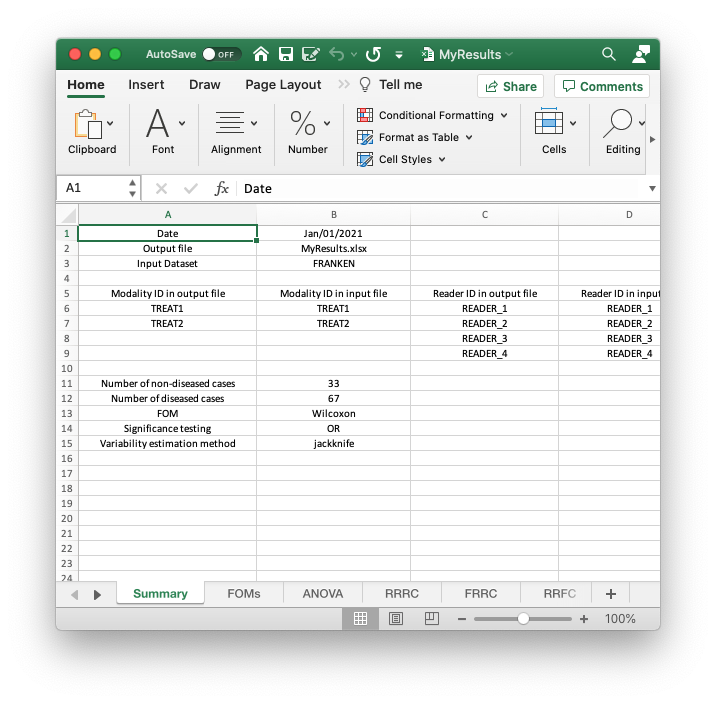
\includegraphics[width=0.5\linewidth,height=0.2\textheight]{R/quick-start/MyResultsSummary} 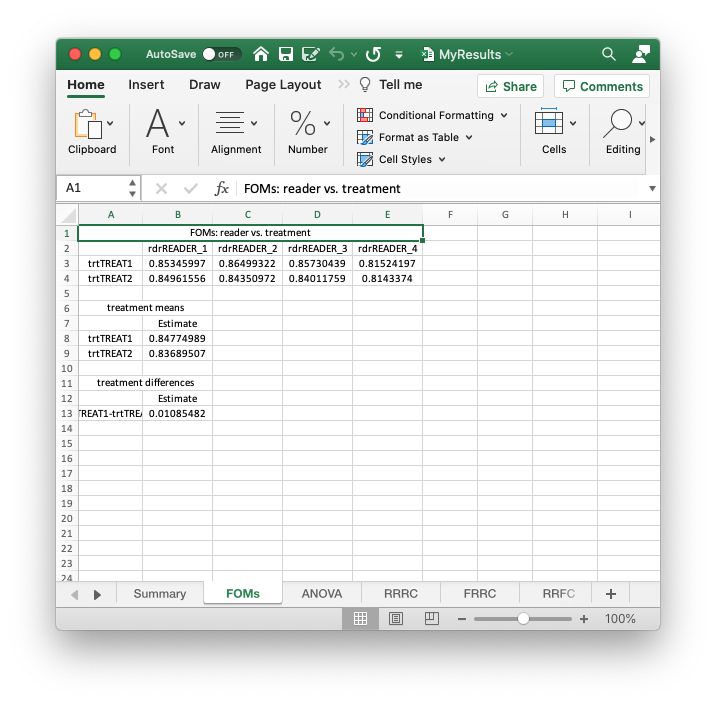
\includegraphics[width=0.5\linewidth,height=0.2\textheight]{R/quick-start/MyResultsFOMs} 

}

\caption{`Summary` and `FOMs` worksheets of Excel file `R/quick-start/MyResults.xlsx`}\label{fig:quick-start-or-xlsx1}
\end{figure}

\begin{figure}

{\centering 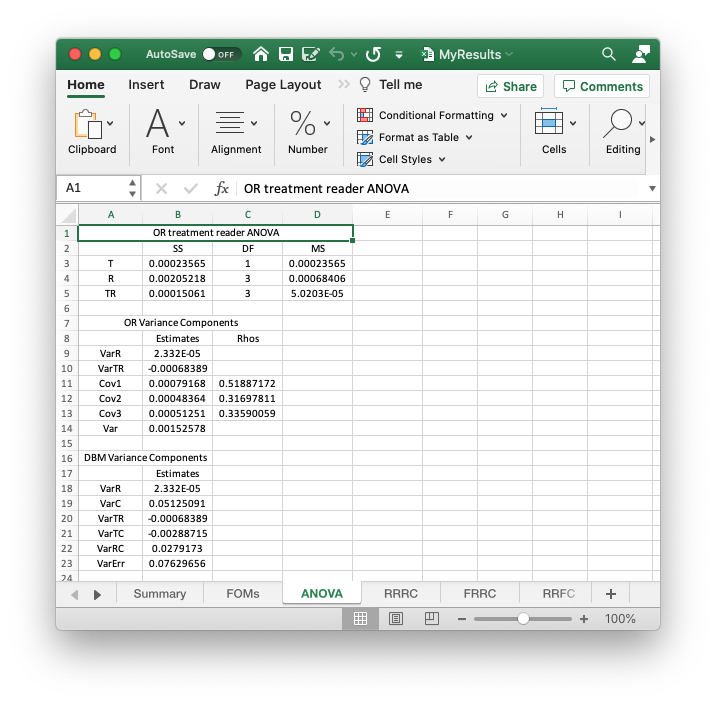
\includegraphics[width=0.5\linewidth,height=0.2\textheight]{R/quick-start/MyResultsANOVA1} 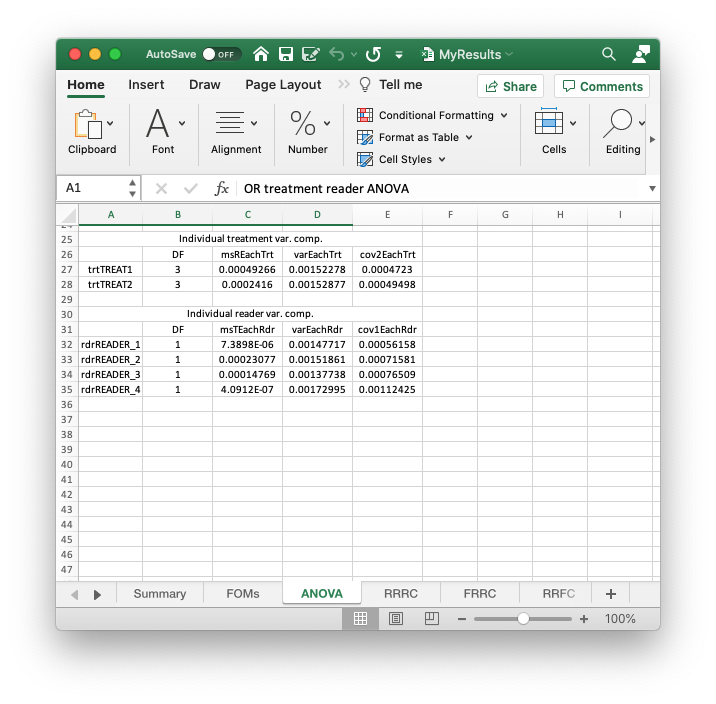
\includegraphics[width=0.5\linewidth,height=0.2\textheight]{R/quick-start/MyResultsANOVA2} 

}

\caption{`ANOVA` worksheet of Excel file `R/quick-start/MyResults.xlsx`}\label{fig:quick-start-or-xlsx2}
\end{figure}

\begin{figure}

{\centering 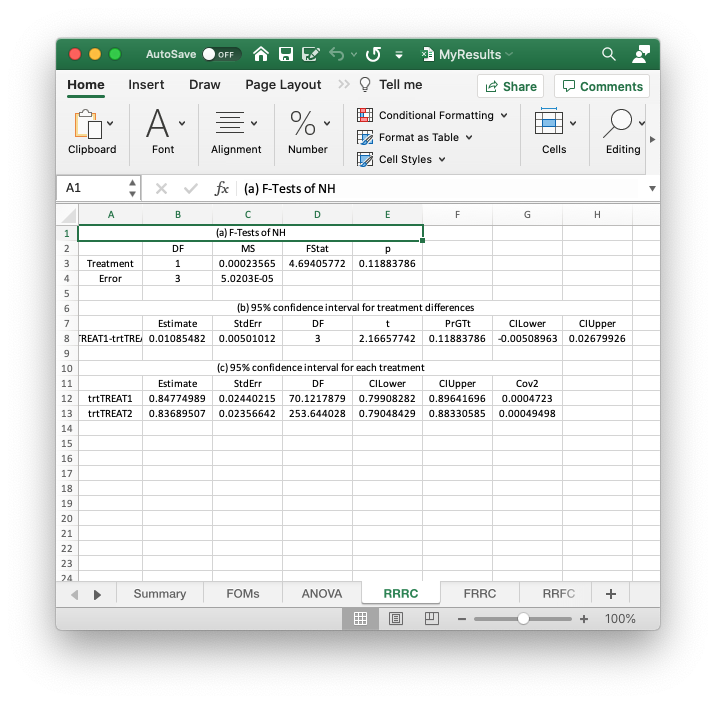
\includegraphics[width=0.5\linewidth,height=0.2\textheight]{R/quick-start/MyResultsRRRC} 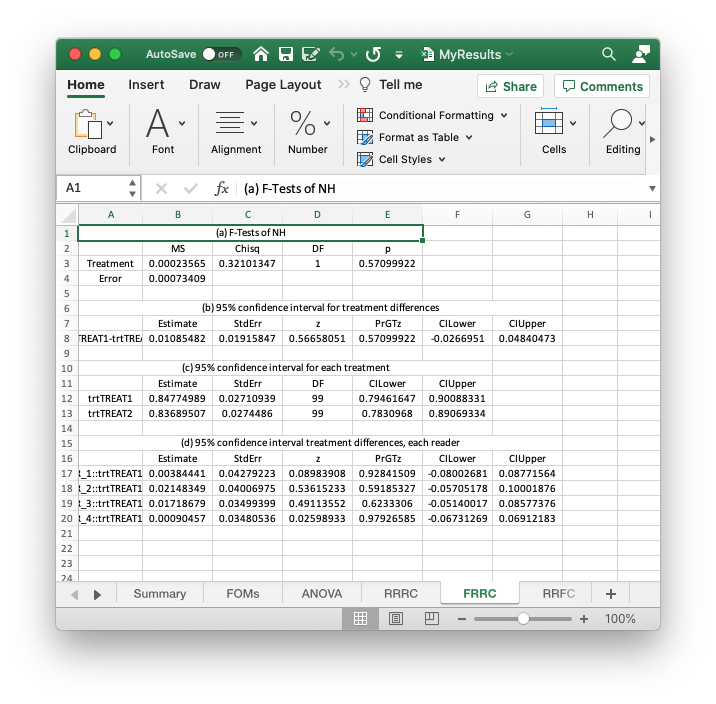
\includegraphics[width=0.5\linewidth,height=0.2\textheight]{R/quick-start/MyResultsFRRC} 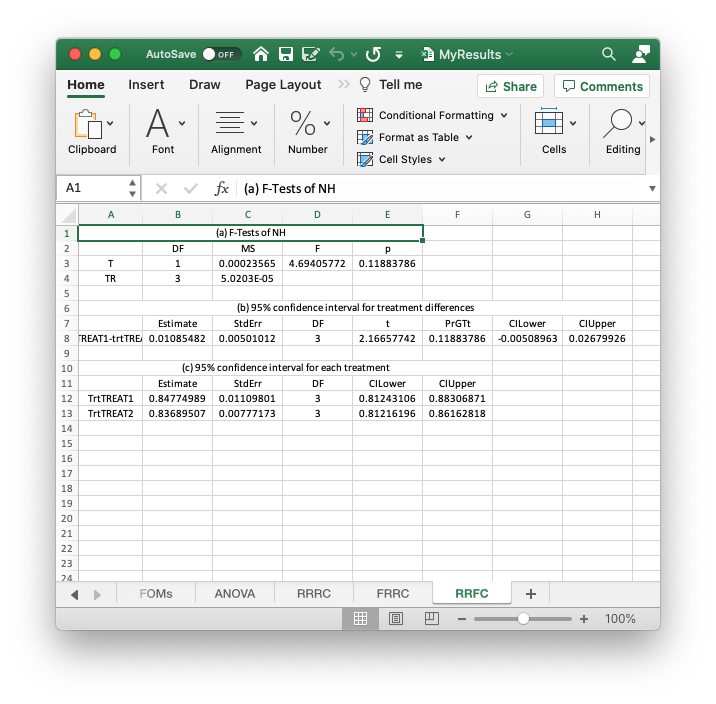
\includegraphics[width=0.5\linewidth,height=0.2\textheight]{R/quick-start/MyResultsRRFC} 

}

\caption{`RRRC`, `FRRC` and `RRFC` worksheets of Excel file `R/quick-start/MyResults.xlsx`}\label{fig:quick-start-or-xlsx3}
\end{figure}

\hypertarget{part-roc-sample-size}{%
\part*{ROC sample size}\label{part-roc-sample-size}}
\addcontentsline{toc}{part}{ROC sample size}

\hypertarget{roc-sample-size-dbm}{%
\chapter{ROC-DBM sample size}\label{roc-sample-size-dbm}}

\hypertarget{roc-sample-size-dbm-how-much-finished}{%
\section{TBA How much finished}\label{roc-sample-size-dbm-how-much-finished}}

80\%

\hypertarget{roc-sample-size-dbm-introduction}{%
\section{Introduction}\label{roc-sample-size-dbm-introduction}}

The question addressed here is ``how many readers and cases'', usually abbreviated to \emph{sample-size}, should one employ to conduct a ``well-planned'' ROC study. The reasons for the quotes will shortly become clear. If cost were no concern, the reply would be: ``as many readers and cases as one can get''. While there are other considerations affecting sample-size, e.g., the data collection paradigm and the the analysis method, this chapter is restricted to the MRMC ROC data collection paradigm with data analyzed by the DBM method described in a previous chapter.

It turns out that provided one can specify conceptually valid effect-sizes between different paradigms (i.e., in the same ``units''), the methods described in this chapter are extensible to other paradigms; see TBA Chapter 19 for sample size estimation for FROC studies. \emph{For this reason it is important to understand the concepts of sample-size estimation in the simpler ROC context.}

For simplicity and practicality, this chapter, and the next, is restricted to analysis of two-treatment data (\(I = 2\)). The purpose of most imaging system assessment studies is to determine, for a given diagnostic task, whether radiologists perform better using a new treatment over the conventional treatment, and whether the difference is statistically significant. Therefore, the two-treatment case is the most common one encountered. While it is possible to extend the methods to more than two treatments, the extensions are not, in my opinion, clinically interesting.

Assume the figure of merit (FOM) \(\theta\) is chosen to be the area AUC under the ROC curve (empirical or fitted is immaterial as far as the formulae are concerned; however, the choice will affect statistical power). The statistical analysis determines the significance level of the study, i.e., the probability or p-value for incorrectly rejecting the null hypothesis (NH) that the two \(\theta\)s are equal: \(NH: \theta_1 = \theta_2\), where the subscripts refer to the two treatments and the bullet represents the average over the reader index. If the p-value is smaller than a pre-specified \(\alpha\), typically set at 5\%, one rejects the NH and declares the treatments different at the \(\alpha\) significance level. Statistical power is the probability of correctly rejecting the null hypothesis when the alternative hypothesis \(AH: \theta_1 \neq \theta_2\) is true, (TBA Chapter 08).

The value of the \emph{true} difference between the treatments, known as the \emph{true effect-size} is, of course, unknown. If it were known, there would be no need to conduct the ROC study. One would simply adopt the treatment with the higher \(\theta\). Sample-size estimation involves making an educated guess regarding the true effect-size , called the \emph{anticipated effect size}, and denoted by \(d\). To quote Harold Kundel \citep{RN1383}: ``any calculation of power amounts to specification of the anticipated effect-size''. Increasing the anticipated effect size will increase statistical power but may represent an unrealistic expectation of the true difference between the treatments, in the sense that it overestimates the ability of technology to achieve this much improvement. Conversely, an unduly small \(d\) might be clinically insignificant, besides requiring a very large sample-size to achieve sufficient statistical power.

Statistical power depends on the magnitude of \(d\) divided by the standard deviation \(\sigma(d)\) of \(d\), i.e.~\(D=\frac{\left | d \right |}{\sigma (d)}\). The sign is relevant as it determines whether the project is worth pursuing at all (see TBA §11.8.4). The ratio is termed \citep{cohen1988statistical} Cohen's D. When this signal-to-noise-ratio-like quantity is large, statistical power approaches 100\%. Reader and case variability and data correlations determine \(\sigma(d)\). No matter how small the anticipated \(d\), as long as it is finite, then, using sufficiently large numbers of readers and cases \(\sigma(d)\) can be made sufficiently small to achieve near 100\% statistical power. Of course, a very small effect-size may not be clinically significant. There is a key difference between \emph{statistical significance} and \emph{clinical significance}. An effect-size in AUC units could be so small, e.g., 0.001, as to be clinically insignificant, but by employing a sufficiently large sample size one could design a study to detect this small - and clinically meaningless - difference with near unit probability, i.e., high statistical power.

What determines clinical significance? A small effect-size, e.g., 0.01 AUC units, could be clinically significant if it applies to a large population, where the small benefit in detection rate is amplified by the number of patients benefiting from the new treatment. In contrast, for an ``orphan'' disease, i.e., one with very low prevalence, an effect-size of 0.05 might not be enough to justify the additional cost of the new treatment. The improvement might have to be 0.1 before it is worth it for a new treatment to be brought to market. One hates to monetize life and death issues, but there is no getting away from it, as cost/benefit issues determine clinical significance. The arbiters of clinical significance are engineers, imaging scientists, clinicians, epidemiologists, insurance companies and those who set government health care policies. The engineers and imaging scientists determine whether the effect-size the clinicians would like is feasible from technical and scientific viewpoints. The clinician determines, based on incidence of disease and other considerations, e.g., altruistic, malpractice, cost of the new device and insurance reimbursement, what effect-size is justifiable. Cohen has suggested that d values of 0.2, 0.5, and 0.8 be considered small, medium, and large, respectively, but he has also argued against their indiscriminate usage. However, after a study is completed, clinicians often find that an effect-size that biostatisticians label as small may, in certain circumstances, be clinically significant and an effect-size that they label as large may in other circumstances be clinically insignificant. Clearly, this is a complex issue. Some suggestions on choosing a clinically significant effect size are made in (TBA §11.12).

Having developed a new imaging modality the R\&D team wishes to compare it to the existing standard with the short-term goal of making a submission to the FDA to allow them to perform pre-market testing of the device. The long-term goal is to commercialize the device. Assume the R\&D team has optimized the device based on physical measurements, (TBA Chapter 01), perhaps supplemented with anecdotal feedback from clinicians based on a few images. Needed at this point is a pilot study. A pilot study, conducted with a relatively small and practical sample size, is intended to provide estimates of different sources of variability and correlations. It also provides an initial estimate of the effect-size, termed the \emph{observed effect-size}, \(d\). Based on results from the pilot the sample-size tools described in this chapter permit estimation of the numbers of readers and cases that will reduce \(\sigma(d)\) sufficiently to achieve the desired power for the larger ``pivotal'' study. {[}A distinction could be made in the notation between observed and anticipated effect sizes, but it will be clear from the context. Later, it will be shown how one can make an educated guess about the anticipated effect size from an observed effect size.{]}

This chapter is concerned with multiple-reader MRMC studies that follow the fully crossed factorial design meaning that each reader interprets a common case-set in all treatments. Since the resulting pairings (i.e., correlations) tend to decrease \(\sigma(d)\) (since the variations occur in tandem, they tend to cancel out in the difference, see (TBA Chapter 09, Introduction), for Dr.~Robert Wagner's sailboat analogy) it yields more statistical power compared to an unpaired design, and consequently this design is frequently used. Two sample-size estimation procedures for MRMC are the Hillis-Berbaum method \citep{RN1476} and the Obuchowski-Rockette \citep{RN1971} method. With recent work by Hillis, the two methods have been shown to be substantially equivalent.

This chapter will focus on the DBM approach. Since it is based on a standard ANOVA model, it is easier to extend the NH testing procedure described in Chapter 09 to the alternative hypothesis, which is relevant for sample size estimation. {[}TBA Online Appendix 11.A shows how to translate the DBM formulae to the OR method \citep{RN2137}.{]}

Given an effect-size, and choosing this wisely is the most difficult part of the process, the method described in this chapter uses pseudovalue variance components estimated by the DBM method to predict sample-sizes (i.e., different combinations of numbers of readers and cases) necessary to achieve a desired power.

\hypertarget{StatPower1}{%
\section{Statistical Power}\label{StatPower1}}

The concept of statistical power was introduced in {[}TBA Chapter 08{]} but is worth repeating. There are two possible decisions following a test of a null hypothesis (NH): reject or fail to reject the NH. Each decision is associated with a probability on an erroneous conclusion. If the NH is true and one rejects it, the probability of the ensuing Type-I error is denoted \(\alpha\). If the NH is false and one fails to reject it, the probability of the ensuing Type II- error is denoted \(\beta\). Statistical power is the complement of \(\beta\), i.e.,

\begin{equation}
Power = 1 - \beta
\label{eq:DefinitionStatPower}
\end{equation}

Typically, one aims for \(\beta = 0.2\) or less, i.e., a statistical power of 80\% or more. Like \(\alpha\) = 0.05, this is a \emph{convention} and more nuanced cost-benefit considerations may cause the researcher to adopt a different value.

\hypertarget{observed-vs.-anticipated-effect-size}{%
\subsection{Observed vs.~anticipated effect-size}\label{observed-vs.-anticipated-effect-size}}

\emph{Assuming no other similar studies have already been conducted with the treatments in question, the observed effect-size, although ``merely an estimate'', is the best information available at the end of the pilot study regarding the value of the true effect-size. From the two previous chapters one knows that the significance testing software will report not only the observed effect-size, but also a 95\% confidence interval associate with it. It will be shown later how one can use this information to make an educated guess regarding the value of the anticipated effect-size.}

\hypertarget{roc-sample-size-dbm-dependence-of-stats-power}{%
\subsection{Dependence of statistical power on estimates of model parameters}\label{roc-sample-size-dbm-dependence-of-stats-power}}

Examination of the expression for , Eqn. (11.5), shows that statistical power increases if:

\begin{itemize}
\tightlist
\item
  The numerator is large. This occurs if: (a) the anticipated effect-size \(d\) is large. Since effect-size enters as the \emph{square}, TBA Eqn. (11.8), it is has a particularly strong effect; (b) If \(J \times K\) is large. Both of these results should be obvious, as a large effect size and a large sample size should result in increased probability of rejecting the NH.
\item
  The denominator is small. The first term in the denominator is \(\left ( \sigma_{\epsilon}^2 + \sigma_{\tau RC}^2 \right )\). These two terms cannot be separated. This is the residual variability of the jackknife pseudovalues. It should make sense that the smaller the variability, the larger is the non-centrality parameter and the statistical power.
\item
  The next term in the denominator is \(K\sigma_{\tau R}^2\), the treatment-reader variance component multiplied by the total number of cases. The reader variance \(\sigma_{R}^2\) has no effect on statistical power, because it has an equal effect on both treatments and cancels out in the difference. Instead, it is the treatment-reader variance \(\sigma_{R}^2\) that contributes ``noise'' tending to confound the estimate of the effect-size.
\item
  The variance components estimated by the ANOVA procedure are realizations of random variables and as such subject to noise (there actually exists a beast such as variance of a variance). The presence of the \(K\) term, usually large, can amplify the effect of noise in the estimate of \(\sigma_{R}^2\), making the sample size estimation procedure less accurate.
\item
  The final term in the denominator is \(J\sigma_{\tau C}^2\). The variance \(\sigma_{C}^2\) has no impact on statistical power, as it cancels out in the difference. The treatment-case variance component introduces ``noise'' into the estimate of the effect size, thereby decreasing power. Since it is multiplied by J, the number of readers, and typically \(J<<K\), the error amplification effect on accuracy of the sample size estimate is not as bad as with the treatment-reader variance component.
\item
  Accuracy of sample size estimation, essentially estimating confidence intervals for statistical power, is addressed in \citep{RN2027}.
\end{itemize}

\hypertarget{roc-sample-size-dbm-RRRC-sample-size-estimation}{%
\subsection{Formulae for random-reader random-case (RRRC) sample size estimation}\label{roc-sample-size-dbm-RRRC-sample-size-estimation}}

\hypertarget{roc-sample-size-dbm-sig-testing}{%
\subsection{Significance testing}\label{roc-sample-size-dbm-sig-testing}}

\hypertarget{roc-sample-size-dbm-pvalue-ci}{%
\subsection{p-value and confidence interval}\label{roc-sample-size-dbm-pvalue-ci}}

\hypertarget{roc-sample-size-dbm-CompareDBM2OR}{%
\subsection{Comparing DBM to Obuchowski and Rockette for single-reader multiple-treatments}\label{roc-sample-size-dbm-CompareDBM2OR}}

Having performed a pilot study and planning to perform a pivotal study, sample size estimation follows the following procedure, which assumes that both reader and case are treated as random factors. Different formulae, described later, apply when either reader or case is treated as a fixed factor.

\begin{itemize}
\tightlist
\item
  Perform DBM analysis on the pilot data. This yields the observed effect size as well as estimates of all relevant variance components and mean squares appearing in TBA Eqn. (11.5) and Eqn. (11.7).
\item
  This is the difficult but critical part: make an educated guess regarding the effect-size, \(d\), that one is interested in ``detecting'' (i.e., hoping to reject the NH with probability \(1-\beta\)). The author prefers the term ``anticipated'' effect-size to ``true'' effect-size (the latter implies knowledge of the true difference between the modalities which, as noted earlier, would obviate the need for a pivotal study).
\item
  Two scenarios are considered below. In the first scenario, the effect-size is assumed equal to that observed in the pilot study, i.e., \(d = d_{obs}\).
\item
  In the second, so-called ``best-case'' scenario, one assumes that the anticipate value of \(d\) is the observed value plus two-sigma of the confidence interval, in the correct direction, of course, i.e., \(d=\left | d_{obs} \right |+2\sigma\). Here \(\sigma\) is one-fourth the width of the 95\% confidence interval for \(d_{obs}\). Anticipating more than \(2\sigma\) greater than the observed effect-size would be overly optimistic. The width of the CI implies that chances are less than 2.5\% that the anticipated value is at or beyond the overly optimistic value. These points will become clearer when example datasets are analyzed below.
\item
  Calculate statistical power using the distribution implied by Eqn. (11.4), to calculate the probability that a random value of the relevant F-statistic will exceed the critical value, as in §11.3.2.
\item
  If power is below the desired or ``target'' power, one tries successively larger value of \(J\) and / or \(K\) until the target power is reached.
\end{itemize}

\hypertarget{roc-sample-size-dbm-FRRC-sample-size-estimation}{%
\section{Formulae for fixed-reader random-case (FRRC) sample size estimation}\label{roc-sample-size-dbm-FRRC-sample-size-estimation}}

It was shown in TBA §9.8.2 that for fixed-reader analysis the non-centrality parameter is defined by:

\begin{equation}
\Delta=\frac{JK\sigma_{\tau}^2}{\sigma_{\epsilon}^2+\sigma_{\tau RC}^2+J\sigma_{\tau C}^2}
\label{eq:DeltaFRRC}
\end{equation}

The sampling distribution of the F-statistic under the AH is:

\begin{equation}
F_{AH|R}\equiv \frac{MST}{MSTC}\sim F_{I-1,(I-1)(K-1),\Delta}
\label{eq:SamplingFFRRC}
\end{equation}

\hypertarget{roc-sample-size-dbm-RRFC-sample-size-estimation}{%
\subsection{Formulae for random-reader fixed-case (RRFC) sample size estimation}\label{roc-sample-size-dbm-RRFC-sample-size-estimation}}

It is shown in TBA §9.9 that for fixed-case analysis the non-centrality parameter is defined by:

\begin{equation}
\Delta=\frac{JK\sigma_{\tau}^2}{\sigma_{\epsilon}^2+\sigma_{\tau RC}^2+K\sigma_{\tau R}^2}
\label{eq:DeltaFRRFC}
\end{equation}

Under the AH, the test statistic is distributed as a non-central F-distribution as follows:

\begin{equation}
F_{AH|C}\equiv \frac{MST}{MSTR}\sim F_{I-1,(I-1)(J-1),\Delta}
\label{eq:SamplingFRRFC}
\end{equation}

\hypertarget{roc-sample-size-dbm-FRRCAnalysis}{%
\subsection{Fixed-reader random-case (FRRC) analysis TBA}\label{roc-sample-size-dbm-FRRCAnalysis}}

It is a realization of a random variable, so one has some leeway in the choice of anticipated effect size - more on this later.
Here \(J^*\) and \(K^*\) refer to the number of readers and cases in the \emph{pilot} study.

\hypertarget{roc-sample-size-dbm-RRFCAnalysis}{%
\subsection{Random-reader fixed-case (RRFC) analysis}\label{roc-sample-size-dbm-RRFCAnalysis}}

\hypertarget{roc-sample-size-dbm-STMRAnalysis}{%
\subsection{Single-treatment multiple-reader analysis}\label{roc-sample-size-dbm-STMRAnalysis}}

\hypertarget{discussionsummary2}{%
\section{Discussion/Summary/2}\label{discussionsummary2}}

\hypertarget{part-froc-analysis}{%
\part*{FROC analysis}\label{part-froc-analysis}}
\addcontentsline{toc}{part}{FROC analysis}

\hypertarget{analyzing-froc-data}{%
\chapter{Analyzing FROC data}\label{analyzing-froc-data}}

\hypertarget{analyzing-froc-data-how-much-finished}{%
\section{TBA How much finished}\label{analyzing-froc-data-how-much-finished}}

10\%

\hypertarget{analyzing-froc-data-intro}{%
\section{Introduction}\label{analyzing-froc-data-intro}}

Analyzing FROC data is, apart from a single difference, very similar to analyzing ROC data. \emph{The crucial difference is the selection of an appropriate location-sensitive figure of merit.} The reason is that the DBMH and ORH methods are applicable to any scalar figure of merit. Any appropriate FROC figure of merit reduces the mark rating data for a single dataset (i.e., a single treatment, a single reader and a number of cases) to a single scalar figure of merit.

The author recommends usage of the weighted AFROC figure of merit, where the lesions should be equally weighted, the default, unless there are strong clinical reasons for assigning unequal weights.

The chapter starts with analysis of a sample FROC dataset, \#4 in Online Chapter 24. Any analysis should start with visualization of the relevant operating characteristic. Extensive examples are given using \texttt{RJafroc} implemented functions. Suggestions are made on how to report the results of a study (the suggestions apply equally to ROC studies). A method called \emph{crossed-treatment analysis}, applicable when one has two treatment factors and their levels are crossed and one wishes to draw conclusions regarding the effect of treatments after averaging over all levels of the treatments.

\hypertarget{analyzing-froc-data-example1}{%
\section{Example 1}\label{analyzing-froc-data-example1}}

The following is a listing of file ``mainAnalyzewAFROC.R''. It performs both wAFROC and inferred ROC analyses of the same dataset and the results are saved to tables similar in structure to the Excel output tables shown for DBMH analysis of ROC data in §9.10.2.

Empirical wAFROC-AUC and ROC-AUC for all combinations of treatments and readers, and reader-averaged AUCs for each treatment (Rdr. Avg.). The weighted AFROC results were obtained from worksheet FOMs in file FedwAfroc.xlsx. The highest rating AUC results were obtained from worksheet FOMs in file FedHrAuc.xlsx. The wAFROC-AUCs are smaller than the corresponding ROC-AUCs.

The datasets that come with this book are described in Online Chapter 24. Four of these are ROC datasets, one an LROC dataset and the rest (nine) are FROC datasets. For non-ROC datasets, the highest rating method was used to infer the corresponding ROC data. The datasets are identified in the code by strings contained in the string-array variable fileNames (line 7 - 8). Line 9 selects the dataset to be analyzed. In the example shown the ``FED'' dataset has been selected. It is a 5 treatment 4 radiologist FROC dataset1 acquired by Dr.~Federica Zanca. Line 13 loads the dataset; this is done internal to the function loadDataFile(). Line 11 constructs the name of the wAFROC file and line 12 does the same for the ROC datafile. Line 15 which ``spills over'' to line 16 without the need for a special continuation character, generates an output file by performing DBMH significance testing (method = ``DBMH'') using fom = ``wAFROC'', i.e., the wAFROC figure of merit -- this is the critical change. If one changes this to fom = ``HrAuc'', lines 19 -- 20, then inferred ROC analysis occurs. In either case the default analysis, i.e., option = ``ALL'' is used, i.e., random-reader random-case (RRRC), fixed-reader random-case (FRRC) and random-reader fixed-case (RRFC). Results are shown below for random-reader random-case only.

The results of wAFROC analysis are saved to FedwAfroc.xlsx and that of inferred ROC analysis are saved to FedHrAuc.xlsx. The output file names need to be explicitly stated as otherwise they would overwrite each other (as a time-saver, checks are made at lines 14 and 18 to determine if the analysis has already been performed, in which case it is skipped).

In the Excel data file the readers are named 1, 3, 4 and 5 -- the software treats the reader names as labels. The author's guess is that for some reason complete data for reader 2 could not be obtained. The renumber = TRUE option has the effect of renumbering the readers 1 through 4. Without renumbering, the output would be aesthetically displeasing, but have no effect on the conclusions.

Figures of merit, empirical wAFROC-AUC and empirical ROC-AUC, and the corresponding reader averages for both analyses are summarized in Table 19.1. The weighted AFROC results were obtained by copy and paste operations from worksheet FOMs in file FedwAfroc.xlsx. The highest rating AUC results were obtained by similar operations from worksheet FOMs in Excel file FedHrAuc.xlsx. As expected, each wAFROC-AUC is smaller than the corresponding ROC-AUC.

Table 19.1: Empirical wAFROC-AUC and ROC-AUC for all combinations of treatments and readers, and reader-averaged AUCs for each treatment (Rdr. Avg.). The weighted AFROC results were obtained from worksheet FOMs in file FedwAfroc.xlsx. The highest rating AUC results were obtained from worksheet FOMs in file FedHrAuc.xlsx. The wAFROC-AUCs are smaller than the corresponding ROC-AUCs.

Table 19.2 shows results for RRRC analysis using the wAFROC-AUC FOM. The overall F-test of the null hypothesis that all treatments have the same reader-averaged FOM, rejected the NH: F(4, 36.8) = 7.8, p = 0.00012 . The numerator degree of freedom ndf is I - 1 = 4. Since the null hypothesis is that all treatments have the same FOM, this implies that at least one pairing of treatments yielded a significant FOM difference. The control for multiple testing is in the formulation of the null hypothesis and no further Bonferroni-like2 correction is needed. To determine which specific pairings are significantly different one examines the p-values (listed under Pr\textgreater t) in the ``95\% CI's FOMs, treatment difference'' portion of the table. It shows that the following differences are significant at alpha = 0.05, namely ``1 -- 3'', ``1 -- 5'', ``2 -- 3'', ``2 -- 5'', ``3 -- 4'' and ``4 -- 5''; these are indicated by asterisks. The values listed under the ``95\% CI's FOMs, each treatment'' portion of the table show that treatment 4 yielded the highest FOM (0.769) followed closely by treatments 2 and 1, while treatment 5 had the least FOM (0.714), slightly worse than treatment 3. This explains why the p-value for the difference 4 - 5 is the smallest (0.00007) of all the listed p-values in the ``95\% CI's FOMs, each treatment'' portion of the table. Each instance where the p-value for the individual treatment comparisons yields a significant p-value is accompanied by a 95\% confidence interval that does not include zero. The two statements of significance, one in terms of a p-value and one in terms of a CI, are equivalent. When it comes to presenting results for treatment FOM differences, I prefer the 95\% CI but some journals insist on a p-value, even when it is not significant. Note that two sequential tests are involved, an overall F-test of the NH that all treatments have the same performance and only if this yields a significant results is one justified in looking at the p-values of individual treatment pairings.

Table 19.2: wAFROC-AUC analysis: results of random-reader random-case (RRRC) analysis, in worksheet ``RRRC''``. {[}ddf = denominator degrees of freedom of F-distribution. df = degrees of freedom of t-distribution. Stderr = standard error. CI = confidence interval. * = Significantly different at alpha = 0.05.{]}

Table 19.3 shows corresponding results for the inferred ROC-AUC FOM. Again the null hypothesis was rejected: F(4, 16.8) = 3.46, p = 0.032. This means at least two treatments have significantly different FOMs. Looking down the table, one sees that the same 6 pairs (as compared to wAFROC analysis) are significantly different, 1 -- 3, 1- 5, etc., as indicated by the asterisks. The last five rows of the table show that treatment 4 had the highest performance while treatment 5 had the lowest performance. At the 5\% significance level, both methods yielded the same significant differences, but this is not always true. While it is incorrect to conclude from a single dataset that a smaller p-value is indicative of higher statistical power, simulation testing under controlled conditions has consistently shown higher statistical power for the wAFROC-AUC FOM3,4 as compared to the inferred ROC-AUC FOM.

Table 19.3: Inferred ROC-AUC analysis: results of random-reader random-case (RRRC) analysis, in worksheet ``RRRC''``. ddf = denominator degrees of freedom of F-distribution. df = degrees of freedom of t-distribution. Stderr = standard error. CI = confidence interval; * = Significantly different at alpha = 0.05.{]}.

\hypertarget{analyzing-froc-data-plotting}{%
\section{TBA Plotting wAFROC and ROC curves}\label{analyzing-froc-data-plotting}}

It is important to display empirical wAFROC/ROC curves, not just for publication purposes, but to get a better feel for the data. Since treatments 4 and 5 showed the largest difference, the corresponding /ROC plots for them are displayed. The code is in file mainwAfrocRocPlots.R.

Sourcing this code yields Fig. 19.1. Plot (A), originating from lines 16 -- 19, shows individual reader wAFROC plots for treatment 4 (solid lines) and treatment 5 (dashed lines). Running the software on one's computer best shows the color-coding. While difficult to see, examination of this plot shows that all readers performed better in treatment 4 than in treatment 5 (i.e., for each color the solid line is above the dashed line). Plot (B), originating from lines 21 -- 25, shows reader-averaged wAFROC plots for treatments 4 (red line, upper curve) and 5 (blue line, lower curve). If one changes, for example, line 19 from print(plot1\(wAFROCPlot) to print(plot1\)wAFROCPoints) the code will output the coordinates of the points describing the curve, which gives the user the option to copy and paste the operating points into alternative plotting software.

Lines 16 -- 19 create plots for all specified treatment-reader combinations. The ``trick'' to creating reader-averaged curves, such as in (B) is defining two list variables, plotT and plotR, at lines 21 -- 22, the first containing the treatments to be plotted, list(4,5), and the second, a list of equal length, containing the arrays of readers to be averaged over, list(c(1:4), c(1:4)). More examples can be found in the help page for PlotEmpiricaOperatingCharacteristics().

Meaningful operating points on the reader average curves cannot be defined. This is because ratings are treatment and reader specific labels, so one cannot for example, average bin counts over all readers to construct a table like ROC Table 4.1 or its AFROC counterpart, Table 13.3.

Instead, the following procedure is used internal to PlotEmpiricaOperatingCharacteristics(). The reader-averaged plot for a specified treatment is obtained by dividing the FPF range from 0 to 1 into finely spaced steps of 0.005. For each FPF value the wLLF values for that treatment are averaged over all readers, yielding the reader-averaged ordinate. Calculating confidence intervals on the reader-averaged curve is possible but cumbersome and unnecessary in my opinion. The relevant information, namely the 95\% confidence interval on the difference in reader-averaged AUCs, is already contained in the program output, see Table 19.2, row labeled ``4 -- 5*``. The difference is 0.05488 with a 95\% confidence interval (0.03018, 0.07957).

Fig. 19.1: FED dataset; (A): individual reader wAFROC plots for treatments 4 and 5. While difficult to see, all readers performed better in treatment 4 as indicated by each colored solid line being above the corresponding dashed lines. (B): reader-averaged wAFROC plots for treatments 4 and 5. The performance superiority of treatment 4 is fairly obvious in this curve. The difference is significant, p = 0.00012.

Inferred ROC plots corresponding to Fig. 19.1 were generated by lines 20-24, i.e., by changing opChType = ``wAFROC'' to opChType = ``ROC'', and print(plot2\(wAFROCPlot) to print(plot2\)ROCPlot), resulting in Fig. 19.2. From Table 19.3 it is seen that the difference in reader-averaged AUCs is 0.04219 with a 95\% confidence interval (0.00727, 0.07711). The observed wAFROC effect-size, 0.05488, is larger than the corresponding inferred ROC effect-size, 0.04219. This is a common observation, but sampling variability compounded with small differences, could give different results.

Fig. 19.2: FED dataset; (A): individual reader ROC plots for treatments 4 and 5. While difficult to see, all readers performed better in treatment 4. (B): reader-averaged ROC plots for treatments 4 and 5. The performance superiority of treatment 4 is fairly obvious in this curve. The difference is significant, p = 0.03054.

\hypertarget{analyzing-froc-data-reporting}{%
\section{Reporting an FROC study}\label{analyzing-froc-data-reporting}}

The methods section should make it clear exactly how the study was conducted. The information should be enough to allow some one else to replicate the study. How many readers, how many cases, how many treatments were used. How was ground truth determined and if the FROC paradigm was used, how were true lesion locations determined? The instructions to the readers should be clearly stated in writing. Precautions to minimize reading order effects should be stated -- usually this is accomplished by interleaving cases from different treatments so that the chances that cases from a particular treatment is always seen first by every reader are minimized. Additionally, images from the same case, but in different treatments, should not be viewed in the same reading session. Reading sessions are usually an hour, and the different sessions should ideally be separated by at least one day. Users generally pay minimal attention to training sessions. It is recommended that at least 25\% of the total number of interpretations be training cases and cases used for training should not be used in the main study. Feedback should be provided during training session to allow the reader to become familiar with the range of difficulty levels regarding diseased and non-diseased cases in the dataset. Deception, e.g., stating a higher prevalence than is actually used, is usually not a good idea. The user-interface should be explained carefully. The best user interface is intuitive, minimizes keystrokes and requires the least explanation.

In publications, the paradigm used to collect the data (ROC, FROC, etc.) and the figure of merit used for analysis should be stated. If FROC, the proximity criterion should be stated. The analysis should state the NH and the alpha of the test, and the desired generalization. The software used and appropriate references should be cited. The results of the overall F-test, the p-value, the observed F-statistic and its degrees of freedom should be stated. If the NH is not rejected, one should cite the observed inter-treatment FOM differences, confidence intervals and p-values and ideally provide preliminary sample size estimates. This information could be useful to other researchers attempting to conduct a larger study. If the NH is rejected, a table of inter-treatment FOM differences such as Table 19.3 should be summarized. Reader averaged plots of the relevant operating characteristics for each treatment should be provided. In FROC studies it is recommended to vary the proximity criterion, perhaps increasing it by a factor of 2, to test if the final conclusions (is NH rejected and if so which treatment is highest) are unaffected.

Assuming the study has been done properly and with sufficiently large number of cases, the results should be published in some form, even if the NH is not rejected. The dearth of datasets to allow reasonable sample size calculations is a real problem in this field. The dataset set should be made available, perhaps on Research Gate, or if communicated to me, they will be included in the Online Appendix material. Datasets acquired via NIH or other government funding must be made available upon request, in an easily decipherable format. Subsequent users of these datasets must cite the original source of the data. Given the high cost of publishing excess pages in some journals, an expanded version, if appropriate for clarity, should be made available using online posting avenues.

\hypertarget{crossed-treatment-analysis}{%
\section{Crossed-treatment analysis}\label{crossed-treatment-analysis}}

This analysis was developed for a particular application6 in which nodule detection in an anthropomorphic chest phantom in computed tomography (CT) was evaluated as a function of tube charge and reconstruction method. The phantom was scanned at 4 values of mAs and images were reconstructed with adaptive iterative dose reduction 3D (AIDR3D) and filtered back projection (FBP). Thus there are two treatment factors and the factors are crossed since for each value of the mAs factor there were two values of the reconstruction algorithm factor. Interest was in determining if whether performance depends on mAs and/or reconstruction method.

In a typical analysis of MRMC ROC or FROC study, treatment is considered as a single factor with I levels, where I is usually small. The figure of merit for treatment i (i =1,2,\ldots,I) and reader j ( j =1,2,\ldots,J) is denoted ; the case set index is suppressed. MRMC analysis compares the observed magnitude of the difference in reader-averaged figures of merit between treatments i and i', , to the estimated standard deviation of the difference. For example, the reader-averaged difference in figures of merit is , where the dot symbol represents the average over the corresponding (reader) index. The standard deviation of the difference is estimated using the DBMH or the ORH method, using for example jackknifing to determine the variance components and/or covariances. With I levels, the number of distinct i vs.~i' comparisons is I (I −1)/2. If the current study were analyzed in this manner, where I =8 (4 levels of mAs and two image reconstruction methods), then this would imply 28 comparisons. The large number of comparisons leads to loss of statistical power in detecting the effect of a specific pair of treatments, and, more importantly, does not inform one of the main points of interest: whether performance depends on mAs and/or reconstruction method. For example, in standard analysis the two reconstruction algorithms might be compared at different mAs levels, and one is in the dark as to which factor (algorithm or mAs) caused the observed significant difference.

Unlike conventional ROC type studies, the images in this study are defined by two factors. The first factor, tube charge, had four levels: 20, 40, 60 and 80 mAs. The second factor, reconstruction method, had two levels: FBP and AIDR3D. The figure of merit is represented by , where represents the levels of the first factor (mAs), and represents the levels of the second factor (reconstruction method), . Two sequential analyses were performed: (i) mAs analysis, where the figure of merit was averaged over (the reconstruction index); and (ii) reconstruction analysis, where the figure of merit was averaged over (the mAs index). For example, the mAs analysis figure of merit is , where the dot represents the average over the reconstruction index, and the corresponding reconstruction analysis figure of merit is , where the dot represents the average over the mAs index. Thus in either analysis, the figure of merit is dependent on a single treatment factor, and therefore standard DBMH or ORH methods apply.

The mAs analysis determines whether tube charge is a significant factor and in this analysis the number of possible comparisons is only six. The reconstruction analysis determines whether AIDR3D offers any advantage over FBP and in this analysis the number of possible comparisons is only one. Multiple testing on the same dataset increases the probability of Type I error, therefore a Bonferroni correction is applied by setting the threshold for declaring significance at 0.025; this is expected to conservatively maintain the overall probability of a Type I error at α = 0.05. Crossed-treatment analysis is used to describe this type of analysis of ROC/FROC data, which yields clearer answers on which of the two factors effects performance. The averaging over the other treatment has the effect of increasing the power of the study in detecting differences in each of the two factors.

Since the phantom is unique, and conclusions are only possible that are specific to this one phantom, the case (or image) factor was regarded as fixed. For this reason only results of random-reader fixed-case analyses are reported.

\hypertarget{analyzing-froc-data-rjafroc-history}{%
\section{Discussion / Summary}\label{analyzing-froc-data-rjafroc-history}}

An IDL (Interactive Data Language, currently marketed by Exelis Visual Information Solutions, www.exelisvis.com) version of JAFROC was first posted to a now obsolete website on 4/16/2004. This software required a license for IDL, which most users did not have. Subsequently, (9/27/2005) a version was posted which allowed analysis using the freely downloadable IDL Virtual Machine software (a method for freely distributing compiled IDL code). On 1/11/2011 the standalone Windows-compatible version was posted (4.0) and the current version is 4.2. JAFROC is windows compatible (XP, Vista and Windows 7, 8 and10).

To our knowledge JAFROC is the only easily accessible software currently available that can analyze FROC data. Workstation software for acquiring ROC and FROC data is available from several sources7-9. The Windows version is no longer actively supported (bugs, if pointed out, will be corrected). Current effort to conduct research and distribute software uses the R platform10. There are several advantages to this. R is an open-source platform - we have already benefited from a bug pointed out by a user . R runs on practically any platform (Windows, OSX, Linux, etc.). Also, developing an R package benefits from other contributed R-packages, which allow easy computation of probability integrals, random number generation, and parallel computing to speed up computations, to name just a few. The drawback with R, and this has to with its open source philosophy, is that one cannot readily integrate existing ROC code, developed on other platforms and other programming languages (specifically, DLLs are not allowed in R). So useful programs like CORROC2 and CBM were coded in C++, since R allows C++ programs to be compiled and included in a package.

Due to the random number of marks per image, data entry in the FROC paradigm is inherently more complicated and error-prone than in ROC analysis, and consequently, and in response to feedback from users, much effort has gone into error checking. The users have especially liked the feature where the program indicates the Excel sheet name and line-number where an error is detected. User-feedback has also been very important in detecting program bugs and inconsistencies in the documentation and developing additional features (e.g., ROI analysis).

Interest in the FROC paradigm is evidenced by the fact that Ref. 3 describing the JAFROC method has been cited over 273 times. Over 25,000 unique visitors have viewed my website, at least 73 have downloaded the software and over 107 publications using JAFROC have appeared. The list is available on my website. JAFROC has been applied to magnetic resonance imaging, virtual computerized tomography colonoscopy, digital tomosynthesis (chest and breast), mammography dose and image processing optimization, computer aided detection (CAD), computerized tomography, and other applications.

Since confusion still appears to exist, especially among statisticians, regarding perceived neglect of intra-image correlations of ratings and how true negatives are handled in FROC analysis11, we close with a quote from respected sources 12 ``(Chakraborty and Berbaum) have presented a solution to the FROC problem using a jackknife resampling approach that respects the correlation structure in the images \ldots{} their paradigm successfully passes a rigorous statistical validation test''. Since 2005 the National Institutes for Health (NIH) has been generous with supporting the research and users of JAFROC have been equally generous with providing their datasets, which have resulted in several collaborations.

\hypertarget{part-froc-sample-size}{%
\part*{FROC sample size}\label{part-froc-sample-size}}
\addcontentsline{toc}{part}{FROC sample size}

\hypertarget{froc-sample-size}{%
\chapter{Sample size estimation for FROC studies}\label{froc-sample-size}}

\hypertarget{froc-sample-size-how-much-finished}{%
\section{TBA How much finished}\label{froc-sample-size-how-much-finished}}

80\%

\hypertarget{overview}{%
\section{Overview}\label{overview}}

This chapter is split into two parts.

\begin{itemize}
\item
  The first part goes into the details of FROC paradigm sample size estimation.
\item
  The second part encapsulates most of the details in a new function \texttt{SsFrocNhRsmModel()}, which encapsulates some of the code in the first part (that relating to building the NH model), thereby making it easier for the user to perform FROC sample size estimation.
\end{itemize}

These parts are independently included in two \texttt{RJafroc} vignettes (on the GitHub \texttt{master} branch, not the CRAN uploaded version). These are located at:

\url{https://dpc10ster.github.io/RJafroc/articles/Ch19Vig1FrocSampleSize.html}

\url{https://dpc10ster.github.io/RJafroc/articles/Ch19Vig2FrocSampleSize.html}

\hypertarget{part-1}{%
\section{Part 1}\label{part-1}}

\hypertarget{froc-sample-size-intro}{%
\subsection{Introduction}\label{froc-sample-size-intro}}

FROC sample size estimation is not fundamentally different from the procedure outlined in TBA Chapter 11 for the ROC paradigm. To recapitulate, based on analysis of a pilot ROC dataset and using a specified FOM, e.g., \texttt{FOM\ =\ Wilcoxon}, and either \texttt{method\ =\ "DBM"} or \texttt{method\ =\ "OR"} for significance testing, one estimates the intrinsic variability of the data expressed in terms of variance components. For DBM analysis, these are the pseudovalue variance components, while for OR analysis these are the FOM treatment-reader variance component and the FOM covariances. The second step is to specify a clinically realistic effect-size, e.g., the anticipated AUC difference between the two modalities. Given these values, the sample size functions implemented in \texttt{RJafroc} (beginning with \texttt{Ss}) allow one to estimate the number of readers and cases necessary to detect (i.e., reject the null hypothesis) the modality AUC difference at specified Type II error rate \(\beta\), typically chosen to be 20\% - corresponding to 80\% statistical power - and specified Type I error rate \(\alpha\), typically chosen to be 5\%.

In FROC analysis the only difference, indeed the critical difference, is the choice of FOM; e.g., \texttt{FOM\ =\ "wAFROC"} instead of the inferred ROC-AUC, \texttt{FOM\ =\ "HrAuc"}. The FROC dataset is analyzed using either the DBM or the OR method. This yields the necessary variance components or the covariance matrix corresponding to the wAFROC-AUC. The next step is to specify the effect-size \textbf{in wAFROC-AUC units}. The ROC-AUC has a historically well-known interpretation: the classification ability at separating diseased patients from non-diseased patients while the wAFROC-AUC does not. Needed is a way of relating the effect-size in ROC-AUC units to one in wAFROC-AUC units: as should be obvious this requires a physical model, e.g., the RSM, that predicts both ROC and wAFROC curves and the respective AUCs.

\begin{enumerate}
\def\labelenumi{\arabic{enumi}.}
\tightlist
\item
  One chooses an ROC-AUC effect-size that is realistic, one that clinicians understand and can therefore participate in, in the effect-size postulation process. Lacking such information I recommend, based on past ROC studies, 0.03 as typical of a small effect size and 0.05 as typical of a moderate effect size.
\item
  One converts the ROC effect-size to a wAFROC-AUC effect-size. The method for this is described in the next section.
\item
  One uses the sample size tools in in \texttt{RJafroc} to determine sample size or power.
\end{enumerate}

\textbf{It is important to recognize is that all quantities have to be in the same units}. When performing ROC analysis, everything (variance components and effect-size) has to be in units of the selected FOM, e.g., \texttt{FOM\ =\ "Wilcoxon"} which is identical to the empirical ROC-AUC. When doing wAFROC analysis, everything has to be in units of the wAFROC-AUC, i.e., \texttt{FOM\ =\ "wAFROC"}. The variance components and effect-size in wAFROC-AUC units will be different from their corresponding ROC counterparts. In particular, as shown next, an ROC-AUC effect-size of 0.05 generally corresponds to a larger effect-size in wAFROC-AUC units. The reason for this is that the range over which wAFROC-AUC can vary, namely 0 to 1, is twice the corresponding ROC-AUC range.

The next section explains the steps used to implement \#2 above.

\hypertarget{relating-an-roc-effect-size-to-a-wafroc-effect-size}{%
\subsection{Relating an ROC effect-size to a wAFROC effect-size}\label{relating-an-roc-effect-size-to-a-wafroc-effect-size}}

\begin{itemize}
\item
  If there are more than two treatments in the pilot dataset extract those treatments that represent null hypothesis data: for example \texttt{DfExtractDataset(dataset,\ trts\ =\ c(1,2,4))} extracts treatments 1, 2 and 4. Save the extracted dataset to \texttt{dataset}. More than two treatments can be used if they have similar FOMs as the averaging/ian procedure described below benefits from more data. However, the final sample size predictions are restricted to two treatments.
\item
  If the original data is FROC, convert it to ROC using \texttt{DfFroc2Roc(dataset)}: this is because \textbf{the RSM fits binned ROC data}. The ROC dataset is \texttt{rocDataset}.
\item
  If the data uses continuous scale ratings, bin the data using \texttt{DfBinDataset(rocDataset,\ opChType\ =\ "ROC")}. The default number of bins should be used. Unlike binning using arbitrarily set thresholds, the thresholds found by \texttt{DfBinDataset} are unique in that they maximize ROC-AUC. The binned dataset is \texttt{rocDatasetB}.
\item
  For each treatment and reader the inferred ROC data is fitted by \texttt{FitRsmRoc()}, see example below, yielding estimates of the RSM \emph{physical} (or pri) parameters (not the \emph{intrinsic} values).
\item
  The following example uses the \emph{first two} treatments of the ``FED'' dataset, \texttt{dataset04}, which is a 5 treatment 4 radiologist FROC dataset acquired by Dr.~Federica Zanca et. al. \citep{RN1882}. The dataset has 5 treatments and 4 readers and 200 cases and was acquired on a 5-point integer scale, i.e., it is already binned. If not one needs to bin the dataset using \texttt{DfBinDataset()}. I need to emphasize this point: \textbf{if the dataset represents continuous ratings, as with a CAD algorithm, one must bin the dataset}.
\item
  The reason for using RSM parameter values only for the first two treatments is that these were found \citep{RN1882} to be almost equivalent (more precisely, the NH could not be rejected for the first two treatments, so it makes sense to regard them as ``almost'' NH treatments.
\item
  The following code block defines the pilot FROC data \texttt{frocData} (corresponding to \texttt{dataset04}, which is the ``FED'' dataset, but with only treatments 1 and 2 extracted, using \texttt{DfExtractDataset()}) and \texttt{rocData}, i.e., the highest-rating ROC dataset inferred from the FROC dataset using \texttt{DfFroc2Roc()}.
\end{itemize}

\begin{Shaded}
\begin{Highlighting}[]
\NormalTok{frocData }\OtherTok{\textless{}{-}} \FunctionTok{DfExtractDataset}\NormalTok{(dataset04, }\AttributeTok{trts =} \FunctionTok{c}\NormalTok{(}\DecValTok{1}\NormalTok{,}\DecValTok{2}\NormalTok{))}
\NormalTok{rocData }\OtherTok{\textless{}{-}} \FunctionTok{DfFroc2Roc}\NormalTok{(frocData)}
\NormalTok{rocDataB }\OtherTok{\textless{}{-}} \FunctionTok{DfBinDataset}\NormalTok{(rocData, }\AttributeTok{opChType =} \StringTok{"ROC"}\NormalTok{) }\CommentTok{\# unnecessary as data is already binned}
\CommentTok{\# but cant hurt}
\end{Highlighting}
\end{Shaded}

The next code block determines \texttt{lesDistr}, the lesion distribution array, which has \texttt{Lmax} (maximum number of lesions per diseased case over the dataset) rows and two columns. The first column contains the integers 1, 2, \ldots, \texttt{Lmax} and the second column contains the fraction of diseased cases with the number of lesions per case specified in the first column. The second column will sum to unity. The RSM fitting algorithm needs to know how lesion-rich the dataset is, as the RSM predicted ROC-AUC depends on the lesion-richness of the dataset. For reasons that will become clear below, one also needs the distribution of the lesion weights. Note that \texttt{lesDist} is determined from the FROC dataset as the lesion-richness information is lost upon conversion to an ROC dataset. The \texttt{PlotRsmOperatingCharacteristics} function used below sets \texttt{relWeights\ =\ 0}, which ensures equally weighted lesions: on cases with one lesion the weight of the lesion is unity, on cases with two lesions the weights of each lesion is 1/2 and on cases with three lesions the weight of each lesion is 1/3, etc.. TBA due to changes in lesDist etc.

\begin{Shaded}
\begin{Highlighting}[]
\NormalTok{lesDistr }\OtherTok{\textless{}{-}} \FunctionTok{UtilLesionDistrVector}\NormalTok{(frocData)}
\FunctionTok{print}\NormalTok{(lesDistr)}
\end{Highlighting}
\end{Shaded}

\begin{verbatim}
## [1] 0.69 0.20 0.11
\end{verbatim}

For this dataset \texttt{Lmax} is 3, and fraction 0.69 of diseased cases have one lesion, fraction 0.2 of diseased cases have two lesions and fraction 0.11 of diseased cases have three lesions.

The next code block determines the number of treatments and readers (\texttt{I} and \texttt{J}) from the dimensions of the \texttt{frocData\$ratings\$NL} array. It creates an array \texttt{RsmParms} to hold the RSM fitted parameter values. For each treatment and reader it applies the fitting algorithm \texttt{FitRsmRoc()}. The first three returned values are \texttt{mu}, \texttt{lambda} and \texttt{nu}, corresponding to RSM parameters \({\mu}\), \({\lambda'}\) and \({\nu'}\).

\begin{Shaded}
\begin{Highlighting}[]
\NormalTok{I }\OtherTok{\textless{}{-}} \FunctionTok{dim}\NormalTok{(frocData}\SpecialCharTok{$}\NormalTok{ratings}\SpecialCharTok{$}\NormalTok{NL)[}\DecValTok{1}\NormalTok{]}
\NormalTok{J }\OtherTok{\textless{}{-}} \FunctionTok{dim}\NormalTok{(frocData}\SpecialCharTok{$}\NormalTok{ratings}\SpecialCharTok{$}\NormalTok{NL)[}\DecValTok{2}\NormalTok{]}
\NormalTok{RsmParms }\OtherTok{\textless{}{-}} \FunctionTok{array}\NormalTok{(}\AttributeTok{dim =} \FunctionTok{c}\NormalTok{(I,J,}\DecValTok{3}\NormalTok{))}
\ControlFlowTok{for}\NormalTok{ (i }\ControlFlowTok{in} \DecValTok{1}\SpecialCharTok{:}\NormalTok{I) \{}
  \ControlFlowTok{for}\NormalTok{ (j }\ControlFlowTok{in} \DecValTok{1}\SpecialCharTok{:}\NormalTok{J)  \{}
\NormalTok{    x1 }\OtherTok{\textless{}{-}} \FunctionTok{FitRsmRoc}\NormalTok{(rocDataB, }\AttributeTok{trt =}\NormalTok{ i, }\AttributeTok{rdr =}\NormalTok{ j, lesDistr)}
\NormalTok{    RsmParms[i,j,}\DecValTok{1}\NormalTok{] }\OtherTok{\textless{}{-}}\NormalTok{ x1[[}\DecValTok{1}\NormalTok{]] }\CommentTok{\# mu}
\NormalTok{    RsmParms[i,j,}\DecValTok{2}\NormalTok{] }\OtherTok{\textless{}{-}}\NormalTok{ x1[[}\DecValTok{2}\NormalTok{]] }\CommentTok{\# lambda}
\NormalTok{    RsmParms[i,j,}\DecValTok{3}\NormalTok{] }\OtherTok{\textless{}{-}}\NormalTok{ x1[[}\DecValTok{3}\NormalTok{]] }\CommentTok{\# nu}
\NormalTok{  \}}
\NormalTok{\}}
\end{Highlighting}
\end{Shaded}

I recommend taking the ian of each of the parameters, over all treatment-reader indices, as representing the average NH dataset. The ian is less sensitive to outliers than the mean.

\begin{Shaded}
\begin{Highlighting}[]
\NormalTok{mu }\OtherTok{\textless{}{-}} \FunctionTok{median}\NormalTok{(RsmParms[,,}\DecValTok{1}\NormalTok{]) }
\NormalTok{lambda }\OtherTok{\textless{}{-}} \FunctionTok{median}\NormalTok{(RsmParms[,,}\DecValTok{2}\NormalTok{])}
\NormalTok{nu }\OtherTok{\textless{}{-}} \FunctionTok{median}\NormalTok{(RsmParms[,,}\DecValTok{3}\NormalTok{])}
\end{Highlighting}
\end{Shaded}

The defining values of the fitting model are \texttt{mu} = 3.3121519, \texttt{lambda} = 1.714368 and \texttt{nu} = 0.7036564. Note that these obey the constraints \texttt{lambda\ \textgreater{}\ 0} and \texttt{0\ \textless{}\ nu\ \textless{}\ 1}. We are now ready to calculate the expected NH FOMs using the ROC -AUC and the wAFROC FOM.

\begin{Shaded}
\begin{Highlighting}[]
\NormalTok{aucRocNH }\OtherTok{\textless{}{-}} \FunctionTok{PlotRsmOperatingCharacteristics}\NormalTok{(mu, lambda, nu, }
                                            \AttributeTok{lesDistr =}\NormalTok{ lesDistr, }\AttributeTok{OpChType =} \StringTok{"ROC"}\NormalTok{)}\SpecialCharTok{$}\NormalTok{aucROC}
\NormalTok{aucwAfrocNH }\OtherTok{\textless{}{-}} \FunctionTok{PlotRsmOperatingCharacteristics}\NormalTok{(mu, lambda, nu, }
                                               \AttributeTok{lesDistr =}\NormalTok{ lesDistr, }\AttributeTok{OpChType =} \StringTok{"wAFROC"}\NormalTok{)}\SpecialCharTok{$}\NormalTok{aucwAFROC}
\end{Highlighting}
\end{Shaded}

\begin{itemize}
\item
  The plotting function \texttt{PlotRsmOperatingCharacteristics()} returns a number of other objects, most importantly the plot, but here we use only the AUC, which is obtained by numerical integration of the predicted operating characteristics.
\item
  One has \texttt{aucRocNH\ =\ 0.8791542} and \texttt{aucwAfrocNH\ =\ 0.7199233}. Note that the wAFROC-FOM is smaller than the ROC-FOM as it includes the localization constraint.
\item
  To induce the alternative hypothesis condition, one increments \(\mu_{NH}\) by \(\Delta_{\mu}\). The resulting ROC-AUC and wAFROC-AUC are calculated, again by numerical integration of the RSM predicted ROC and wAFROC curves, leading to the corresponding effect-sizes (note that in each equation below one takes the difference between the AH value minus the NH value):
\item
  The next step is to calculate the effect size (new value minus the NH value) using ROC and wAFROC FOMs for a series of specified \texttt{deltaMu} values. This generates values that can be used to interpolate a wAFROC effect size for a specified ROC effect size.
\end{itemize}

\begin{Shaded}
\begin{Highlighting}[]
\NormalTok{deltaMu }\OtherTok{\textless{}{-}} \FunctionTok{seq}\NormalTok{(}\FloatTok{0.01}\NormalTok{, }\FloatTok{0.2}\NormalTok{, }\FloatTok{0.01}\NormalTok{) }\CommentTok{\# values of deltaMu to scan below}
\NormalTok{esRoc }\OtherTok{\textless{}{-}} \FunctionTok{array}\NormalTok{(}\AttributeTok{dim =} \FunctionTok{length}\NormalTok{(deltaMu));eswAfroc }\OtherTok{\textless{}{-}} \FunctionTok{array}\NormalTok{(}\AttributeTok{dim =} \FunctionTok{length}\NormalTok{(deltaMu))}
\ControlFlowTok{for}\NormalTok{ (i }\ControlFlowTok{in} \DecValTok{1}\SpecialCharTok{:}\FunctionTok{length}\NormalTok{(deltaMu)) \{}
\NormalTok{  esRoc[i] }\OtherTok{\textless{}{-}} \FunctionTok{PlotRsmOperatingCharacteristics}\NormalTok{(}
\NormalTok{    mu }\SpecialCharTok{+}\NormalTok{ deltaMu[i], lambda, nu, }\AttributeTok{lesDistr =}\NormalTok{ lesDistr, }\AttributeTok{OpChType =} \StringTok{"ROC"}\NormalTok{)}\SpecialCharTok{$}\NormalTok{aucROC }\SpecialCharTok{{-}}\NormalTok{ aucRocNH}
\NormalTok{  eswAfroc[i] }\OtherTok{\textless{}{-}} \FunctionTok{PlotRsmOperatingCharacteristics}\NormalTok{(}
\NormalTok{    mu}\SpecialCharTok{+}\NormalTok{ deltaMu[i], lambda, nu, }\AttributeTok{lesDistr =}\NormalTok{ lesDistr, }\AttributeTok{OpChType =} \StringTok{"wAFROC"}\NormalTok{)}\SpecialCharTok{$}\NormalTok{aucwAFROC }\SpecialCharTok{{-}}\NormalTok{ aucwAfrocNH}
  \FunctionTok{cat}\NormalTok{(}\StringTok{"ES\_ROC = "}\NormalTok{, esRoc[i], }\StringTok{", ES\_wAFROC = "}\NormalTok{, eswAfroc[i],}\StringTok{"}\SpecialCharTok{\textbackslash{}n}\StringTok{"}\NormalTok{)}
\NormalTok{\}}
\end{Highlighting}
\end{Shaded}

\begin{verbatim}
## ES_ROC =  0.0001500649 , ES_wAFROC =  0.000189712 
## ES_ROC =  0.0002978454 , ES_wAFROC =  0.0003764812 
## ES_ROC =  0.0004433681 , ES_wAFROC =  0.0005603432 
## ES_ROC =  0.0005866597 , ES_wAFROC =  0.0007413331 
## ES_ROC =  0.0007277463 , ES_wAFROC =  0.0009194859 
## ES_ROC =  0.0008666543 , ES_wAFROC =  0.001094837 
## ES_ROC =  0.001003409 , ES_wAFROC =  0.00126742 
## ES_ROC =  0.001138038 , ES_wAFROC =  0.001437269 
## ES_ROC =  0.001270565 , ES_wAFROC =  0.00160442 
## ES_ROC =  0.001401017 , ES_wAFROC =  0.001768904 
## ES_ROC =  0.001529418 , ES_wAFROC =  0.001930757 
## ES_ROC =  0.001655794 , ES_wAFROC =  0.002090012 
## ES_ROC =  0.00178017 , ES_wAFROC =  0.002246701 
## ES_ROC =  0.00190257 , ES_wAFROC =  0.002400857 
## ES_ROC =  0.002023021 , ES_wAFROC =  0.002552513 
## ES_ROC =  0.002141544 , ES_wAFROC =  0.002701702 
## ES_ROC =  0.002258166 , ES_wAFROC =  0.002848455 
## ES_ROC =  0.002372911 , ES_wAFROC =  0.002992804 
## ES_ROC =  0.002485801 , ES_wAFROC =  0.00313478 
## ES_ROC =  0.002596862 , ES_wAFROC =  0.003274416
\end{verbatim}

Here is a plot of wAFROC effect size (y-axis) vs.~ROC effect size.

\begin{Shaded}
\begin{Highlighting}[]
\NormalTok{df }\OtherTok{\textless{}{-}} \FunctionTok{data.frame}\NormalTok{(}\AttributeTok{es\_ROC =}\NormalTok{ esRoc, }\AttributeTok{es\_wAFROC =}\NormalTok{ eswAfroc)}
\NormalTok{p }\OtherTok{\textless{}{-}} \FunctionTok{ggplot}\NormalTok{(}\AttributeTok{data =}\NormalTok{ df, }\FunctionTok{aes}\NormalTok{(}\AttributeTok{x =}\NormalTok{ es\_ROC, }\AttributeTok{y =}\NormalTok{ es\_wAFROC)) }\SpecialCharTok{+}
  \FunctionTok{geom\_smooth}\NormalTok{(}\AttributeTok{method =} \StringTok{"lm"}\NormalTok{, }\AttributeTok{se =} \ConstantTok{FALSE}\NormalTok{, }\AttributeTok{color =} \StringTok{"black"}\NormalTok{, }\AttributeTok{formula =}\NormalTok{ y }\SpecialCharTok{\textasciitilde{}}\NormalTok{ x) }\SpecialCharTok{+}
  \FunctionTok{geom\_point}\NormalTok{(}\AttributeTok{size =} \DecValTok{4}\NormalTok{) }\SpecialCharTok{+}
  \FunctionTok{scale\_color\_manual}\NormalTok{(}\AttributeTok{values =} \StringTok{"black"}\NormalTok{) }\SpecialCharTok{+} 
  \FunctionTok{theme}\NormalTok{(}\AttributeTok{axis.title.y =} \FunctionTok{element\_text}\NormalTok{(}\AttributeTok{size =} \DecValTok{10}\NormalTok{,}\AttributeTok{face=}\StringTok{"bold"}\NormalTok{),}
        \AttributeTok{axis.title.x =} \FunctionTok{element\_text}\NormalTok{(}\AttributeTok{size =} \DecValTok{10}\NormalTok{,}\AttributeTok{face=}\StringTok{"bold"}\NormalTok{)) }\SpecialCharTok{+}
  \FunctionTok{scale\_x\_continuous}\NormalTok{(}\AttributeTok{expand =} \FunctionTok{c}\NormalTok{(}\DecValTok{0}\NormalTok{, }\DecValTok{0}\NormalTok{)) }\SpecialCharTok{+} 
  \FunctionTok{scale\_y\_continuous}\NormalTok{(}\AttributeTok{expand =} \FunctionTok{c}\NormalTok{(}\DecValTok{0}\NormalTok{, }\DecValTok{0}\NormalTok{)) }
\FunctionTok{print}\NormalTok{(p)}
\end{Highlighting}
\end{Shaded}

\begin{center}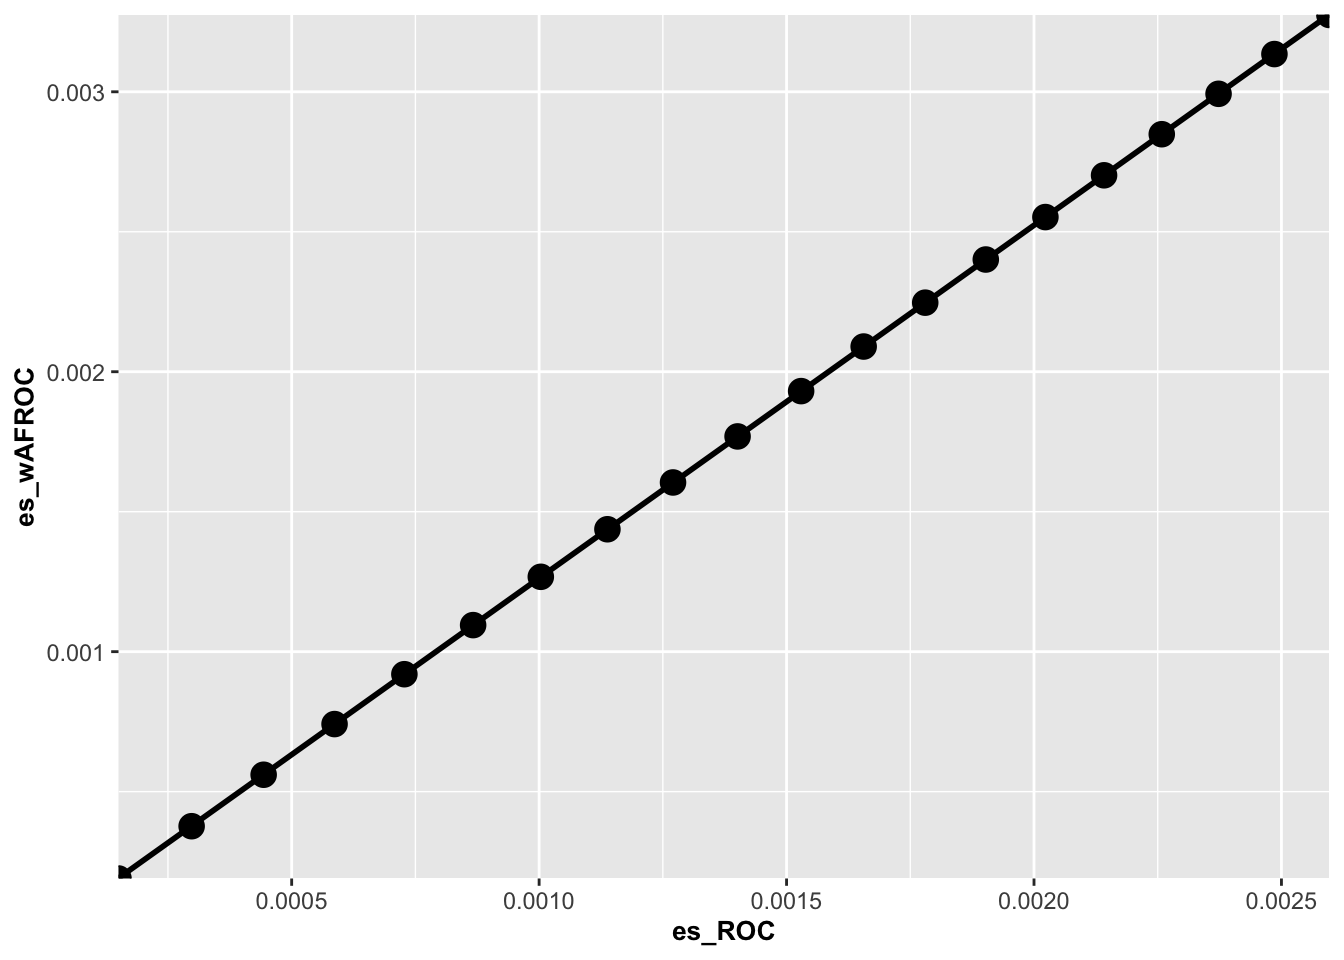
\includegraphics{19-froc-sample-size_files/figure-latex/unnamed-chunk-7-1} \end{center}

The plot is very close to linear. This makes it easy to design an interpolation function. In the following code block the first line fits \texttt{eswAfroc} vs.~\texttt{esRoc} using the linear model \texttt{lm()} function constrained to pass through the origin (the minus one): \texttt{scaleFactor\ \textless{}-\ lm(eswAfroc\ \textasciitilde{}\ -1\ +\ esRoc)}. One expects this constraint since for \texttt{deltaMu\ =\ 0} the effect size must be zero no matter how it is measured.

\begin{Shaded}
\begin{Highlighting}[]
\NormalTok{scaleFactor}\OtherTok{\textless{}{-}}\FunctionTok{lm}\NormalTok{(eswAfroc}\SpecialCharTok{\textasciitilde{}{-}}\DecValTok{1}\SpecialCharTok{+}\NormalTok{esRoc) }\CommentTok{\# fit values to straight line thru origin}
\NormalTok{effectSizeROC }\OtherTok{\textless{}{-}} \FunctionTok{seq}\NormalTok{(}\FloatTok{0.01}\NormalTok{, }\FloatTok{0.1}\NormalTok{, }\FloatTok{0.01}\NormalTok{)}
\NormalTok{effectSizewAFROC }\OtherTok{\textless{}{-}}\NormalTok{ effectSizeROC}\SpecialCharTok{*}\NormalTok{scaleFactor}\SpecialCharTok{$}\NormalTok{coefficients[}\DecValTok{1}\NormalTok{] }\CommentTok{\# r2 = summary(scaleFactor)$r.squared}
\end{Highlighting}
\end{Shaded}

The slope of the zero-intercept constrained straight line fit is \texttt{scaleFactor} = 1.2617239 and the squared correlation coefficient is \texttt{R2} = 0.9999997. Therefore, the conversion from ROC to wAFROC effect size is: \texttt{effectSizewAFROC\ =\ scaleFactor\ *\ effectSizeROC}. \textbf{The wAFROC effect size is twice the ROC effect size.} All that remains is to calculate the variance components using the two FOMs.

\hypertarget{computing-the-respective-variance-components}{%
\subsection{Computing the respective variance components}\label{computing-the-respective-variance-components}}

The code block applies \texttt{StSignificanceTesting()} to \texttt{rocData} and \texttt{frocData}, using the appropriate FOM, and extracts the variance components.

\begin{Shaded}
\begin{Highlighting}[]
\NormalTok{temp1 }\OtherTok{\textless{}{-}} \FunctionTok{StSignificanceTesting}\NormalTok{(rocData, }\AttributeTok{FOM =} \StringTok{"Wilcoxon"}\NormalTok{, }\AttributeTok{method =} \StringTok{"DBM"}\NormalTok{, }\AttributeTok{analysisOption =} \StringTok{"RRRC"}\NormalTok{)}
\NormalTok{temp2 }\OtherTok{\textless{}{-}} \FunctionTok{StSignificanceTesting}\NormalTok{(frocData, }\AttributeTok{FOM =} \StringTok{"wAFROC"}\NormalTok{, }\AttributeTok{method =} \StringTok{"DBM"}\NormalTok{, }\AttributeTok{analysisOption =} \StringTok{"RRRC"}\NormalTok{)}
\NormalTok{varCompROC }\OtherTok{\textless{}{-}}\NormalTok{ temp1}\SpecialCharTok{$}\NormalTok{ANOVA}\SpecialCharTok{$}\NormalTok{VarCom}
\NormalTok{varCompwAFROC }\OtherTok{\textless{}{-}}\NormalTok{ temp2}\SpecialCharTok{$}\NormalTok{ANOVA}\SpecialCharTok{$}\NormalTok{VarCom}
\end{Highlighting}
\end{Shaded}

The observed wAFROC effect-size is -0.00685625. This is a very small effect size; the corresponding ROC effect-size is -0.0051; the sign does not affect the calculations, which is too small to reach 80\% power. It is not surprising that the study \citep{RN1882} did not find a significant difference between these two treatments

The respective variance components are:

\begin{Shaded}
\begin{Highlighting}[]
\FunctionTok{print}\NormalTok{(varCompROC)}
\end{Highlighting}
\end{Shaded}

\begin{verbatim}
##            Estimates
## VarR   0.00082773798
## VarC   0.03812334734
## VarTR  0.00015265067
## VarTC  0.00964432675
## VarRC  0.00354419640
## VarErr 0.09484636574
\end{verbatim}

\begin{Shaded}
\begin{Highlighting}[]
\FunctionTok{print}\NormalTok{(varCompwAFROC)}
\end{Highlighting}
\end{Shaded}

\begin{verbatim}
##             Estimates
## VarR    0.00185422886
## VarC    0.06117804981
## VarTR  -0.00044392794
## VarTC   0.01016518621
## VarRC   0.01355883396
## VarErr  0.09672559908
\end{verbatim}

Only terms involving treatment are relevant to sample size. The wAFROC \texttt{varTC} and \texttt{varErr} values are slightly larger than the ROC ones - as expected - because the range of the wAFROC FOM is twice that of the ROC FOM.

\hypertarget{comparing-roc-power-to-wafroc-power-for-equivalent-effect-sizes}{%
\subsection{Comparing ROC power to wAFROC power for equivalent effect-sizes}\label{comparing-roc-power-to-wafroc-power-for-equivalent-effect-sizes}}

We are now ready to compare ROC and wAFROC powers for equivalent effect sizes. The following example is for 5 readers (\texttt{JPivot}) and 100 cases (\texttt{KPivot}) in the \textbf{pivotal study}.

\begin{Shaded}
\begin{Highlighting}[]
\NormalTok{powerROC }\OtherTok{\textless{}{-}} \FunctionTok{array}\NormalTok{(}\AttributeTok{dim =} \FunctionTok{length}\NormalTok{(effectSizeROC));powerwAFROC }\OtherTok{\textless{}{-}} \FunctionTok{array}\NormalTok{(}\AttributeTok{dim =} \FunctionTok{length}\NormalTok{(effectSizeROC))}

\NormalTok{JPivot }\OtherTok{\textless{}{-}} \DecValTok{5}\NormalTok{;KPivot }\OtherTok{\textless{}{-}} \DecValTok{100}
\ControlFlowTok{for}\NormalTok{ (i }\ControlFlowTok{in} \DecValTok{1}\SpecialCharTok{:}\FunctionTok{length}\NormalTok{(effectSizeROC)) \{}
\NormalTok{  varYTR }\OtherTok{\textless{}{-}}\NormalTok{ varCompROC[}\StringTok{"VarTR"}\NormalTok{,}\StringTok{"Estimates"}\NormalTok{] }\CommentTok{\# these are pseudovalue based variance components assuming FOM = "Wilcoxon"}
\NormalTok{  varYTC }\OtherTok{\textless{}{-}}\NormalTok{ varCompROC[}\StringTok{"VarTC"}\NormalTok{,}\StringTok{"Estimates"}\NormalTok{]}
\NormalTok{  varYEps }\OtherTok{\textless{}{-}}\NormalTok{ varCompROC[}\StringTok{"VarErr"}\NormalTok{,}\StringTok{"Estimates"}\NormalTok{]}
\NormalTok{  ret }\OtherTok{\textless{}{-}} \FunctionTok{SsPowerGivenJK}\NormalTok{(}\AttributeTok{dataset =} \ConstantTok{NULL}\NormalTok{, }\AttributeTok{FOM =} \StringTok{"Wilcoxon"}\NormalTok{, }\AttributeTok{J =}\NormalTok{ JPivot, }\AttributeTok{K =}\NormalTok{ KPivot, }\AttributeTok{analysisOption =} \StringTok{"RRRC"}\NormalTok{, }\AttributeTok{effectSize =}\NormalTok{ effectSizeROC[i], }\AttributeTok{method =} \StringTok{"DBM"}\NormalTok{, }\AttributeTok{LegacyCode =} \ConstantTok{TRUE}\NormalTok{, }
        \FunctionTok{list}\NormalTok{(}\AttributeTok{VarTR =}\NormalTok{ varYTR, }\AttributeTok{VarTC =}\NormalTok{ varYTC, }\AttributeTok{VarErr =}\NormalTok{ varYEps))}
\NormalTok{  powerROC[i] }\OtherTok{\textless{}{-}}\NormalTok{ ret}\SpecialCharTok{$}\NormalTok{powerRRRC}
  
\NormalTok{  varYTR }\OtherTok{\textless{}{-}}\NormalTok{ varCompwAFROC[}\StringTok{"VarTR"}\NormalTok{,}\StringTok{"Estimates"}\NormalTok{] }\CommentTok{\# these are pseudovalue based variance components assuming FOM = "wAFROC"}
\NormalTok{  varYTC }\OtherTok{\textless{}{-}}\NormalTok{ varCompwAFROC[}\StringTok{"VarTC"}\NormalTok{,}\StringTok{"Estimates"}\NormalTok{]}
\NormalTok{  varYEps }\OtherTok{\textless{}{-}}\NormalTok{ varCompwAFROC[}\StringTok{"VarErr"}\NormalTok{,}\StringTok{"Estimates"}\NormalTok{]}
\NormalTok{  ret }\OtherTok{\textless{}{-}} \FunctionTok{SsPowerGivenJK}\NormalTok{(}\AttributeTok{dataset =} \ConstantTok{NULL}\NormalTok{, }\AttributeTok{FOM =} \StringTok{"Wilcoxon"}\NormalTok{, }\AttributeTok{J =}\NormalTok{ JPivot, }\AttributeTok{K =}\NormalTok{ KPivot, }\AttributeTok{analysisOption =} \StringTok{"RRRC"}\NormalTok{, }\AttributeTok{effectSize =}\NormalTok{ effectSizewAFROC[i], }\AttributeTok{method =} \StringTok{"DBM"}\NormalTok{, }\AttributeTok{LegacyCode =} \ConstantTok{TRUE}\NormalTok{, }
        \FunctionTok{list}\NormalTok{(}\AttributeTok{VarTR =}\NormalTok{ varYTR, }\AttributeTok{VarTC =}\NormalTok{ varYTC, }\AttributeTok{VarErr =}\NormalTok{ varYEps))}
\NormalTok{  powerwAFROC[i] }\OtherTok{\textless{}{-}}\NormalTok{ ret}\SpecialCharTok{$}\NormalTok{powerRRRC}
  
  \FunctionTok{cat}\NormalTok{(}\StringTok{"ROC{-}ES = "}\NormalTok{, effectSizeROC[i], }\StringTok{", wAFROC{-}ES = "}\NormalTok{, effectSizewAFROC[i], }
      \StringTok{", Power{-}ROC = "}\NormalTok{, powerROC[i], }\StringTok{", Power{-}wAFROC = "}\NormalTok{, powerwAFROC[i], }\StringTok{"}\SpecialCharTok{\textbackslash{}n}\StringTok{"}\NormalTok{)}
\NormalTok{\}}
\end{Highlighting}
\end{Shaded}

\begin{verbatim}
## ROC-ES =  0.01 , wAFROC-ES =  0.012617239 , Power-ROC =  0.064430457 , Power-wAFROC =  0.075439644 
## ROC-ES =  0.02 , wAFROC-ES =  0.025234479 , Power-ROC =  0.10878897 , Power-wAFROC =  0.15449773 
## ROC-ES =  0.03 , wAFROC-ES =  0.037851718 , Power-ROC =  0.18471152 , Power-wAFROC =  0.28797922 
## ROC-ES =  0.04 , wAFROC-ES =  0.050468957 , Power-ROC =  0.29079274 , Power-wAFROC =  0.4612966 
## ROC-ES =  0.05 , wAFROC-ES =  0.063086196 , Power-ROC =  0.41954431 , Power-wAFROC =  0.6420946 
## ROC-ES =  0.06 , wAFROC-ES =  0.075703436 , Power-ROC =  0.55738123 , Power-wAFROC =  0.79495349 
## ROC-ES =  0.07 , wAFROC-ES =  0.088320675 , Power-ROC =  0.68816012 , Power-wAFROC =  0.90003872 
## ROC-ES =  0.08 , wAFROC-ES =  0.10093791 , Power-ROC =  0.79836108 , Power-wAFROC =  0.95891383 
## ROC-ES =  0.09 , wAFROC-ES =  0.11355515 , Power-ROC =  0.88095077 , Power-wAFROC =  0.98585038 
## ROC-ES =  0.1 , wAFROC-ES =  0.12617239 , Power-ROC =  0.93606799 , Power-wAFROC =  0.9959336
\end{verbatim}

Since the wAFROC effect size is about a factor of two larger than the ROC effect size, wAFROC power is larger than that for ROC. The effect is magnified as the effect size enters as the square in the formula for the power (this overwhelms the slight increase in variability of wAFROC-FOM relative to ROC-FOM noted previously). The following is a plot of the respective powers.

\begin{Shaded}
\begin{Highlighting}[]
\NormalTok{df }\OtherTok{\textless{}{-}} \FunctionTok{data.frame}\NormalTok{(}\AttributeTok{power\_ROC =}\NormalTok{ powerROC, }\AttributeTok{power\_wAFROC =}\NormalTok{ powerwAFROC)}
\NormalTok{p }\OtherTok{\textless{}{-}} \FunctionTok{ggplot}\NormalTok{(}\AttributeTok{mapping =} \FunctionTok{aes}\NormalTok{(}\AttributeTok{x =}\NormalTok{ power\_ROC, }\AttributeTok{y =}\NormalTok{ power\_wAFROC)) }\SpecialCharTok{+}
  \FunctionTok{geom\_line}\NormalTok{(}\AttributeTok{data =}\NormalTok{ df, }\AttributeTok{size =} \DecValTok{2}\NormalTok{)}\SpecialCharTok{+}
  \FunctionTok{scale\_color\_manual}\NormalTok{(}\AttributeTok{values =} \StringTok{"black"}\NormalTok{) }\SpecialCharTok{+} 
  \FunctionTok{theme}\NormalTok{(}\AttributeTok{axis.title.y =} \FunctionTok{element\_text}\NormalTok{(}\AttributeTok{size =} \DecValTok{10}\NormalTok{,}\AttributeTok{face=}\StringTok{"bold"}\NormalTok{),}
        \AttributeTok{axis.title.x =} \FunctionTok{element\_text}\NormalTok{(}\AttributeTok{size =} \DecValTok{10}\NormalTok{,}\AttributeTok{face=}\StringTok{"bold"}\NormalTok{))  }\SpecialCharTok{+}
  \FunctionTok{scale\_x\_continuous}\NormalTok{(}\AttributeTok{expand =} \FunctionTok{c}\NormalTok{(}\DecValTok{0}\NormalTok{, }\DecValTok{0}\NormalTok{)) }\SpecialCharTok{+} 
  \FunctionTok{scale\_y\_continuous}\NormalTok{(}\AttributeTok{expand =} \FunctionTok{c}\NormalTok{(}\DecValTok{0}\NormalTok{, }\DecValTok{0}\NormalTok{))}
\end{Highlighting}
\end{Shaded}

\begin{verbatim}
## Warning: Using `size` aesthetic for lines was deprecated in ggplot2 3.4.0.
## i Please use `linewidth` instead.
## This warning is displayed once every 8 hours.
## Call `lifecycle::last_lifecycle_warnings()` to see where this warning was
## generated.
\end{verbatim}

\begin{Shaded}
\begin{Highlighting}[]
\FunctionTok{print}\NormalTok{(p)}
\end{Highlighting}
\end{Shaded}

\begin{center}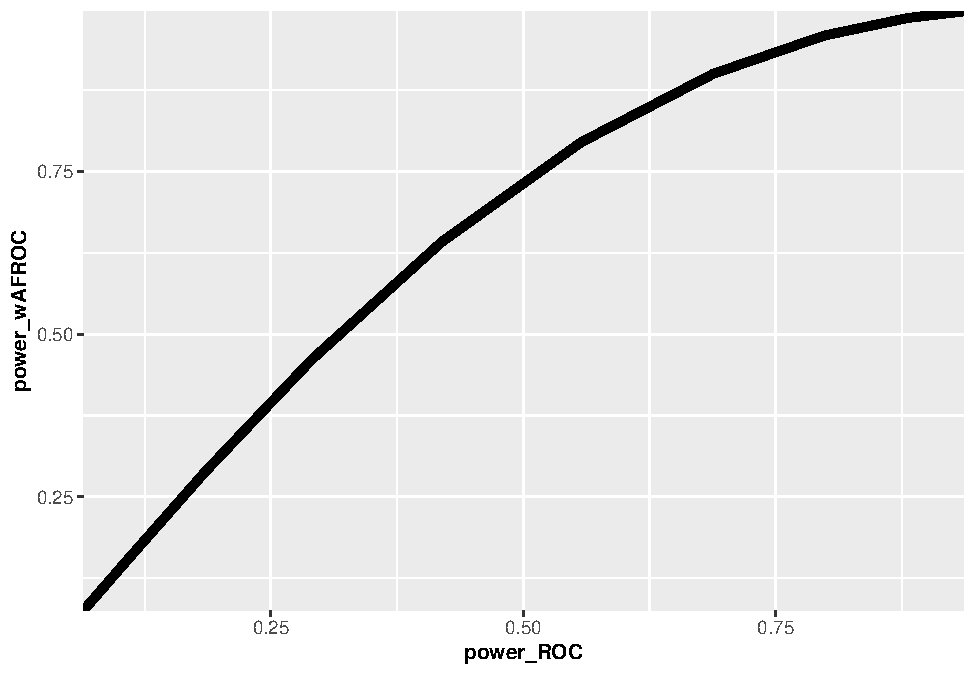
\includegraphics{19-froc-sample-size_files/figure-latex/unnamed-chunk-12-1} \end{center}

\hypertarget{part-2}{%
\section{Part 2}\label{part-2}}

\hypertarget{introduction}{%
\subsection{Introduction}\label{introduction}}

This example uses the FED dataset as a pilot FROC study and function \texttt{SsFrocNhRsmModel()} to construct the NH model (encapsulating some of the code in the first part).

\hypertarget{constructing-the-nh-model-for-the-dataset}{%
\subsection{Constructing the NH model for the dataset}\label{constructing-the-nh-model-for-the-dataset}}

One starts by extracting the first two treatments from \texttt{dataset04}, which represent the NH dataset, see previous part. Next one constructs the NH model - note that the lesion distribution \texttt{lesDistr} can be specified here independently of that in the pilot dataset. This allows some control over selection of the diseased cases in the pivotal study.

\begin{Shaded}
\begin{Highlighting}[]
\NormalTok{lesDistr }\OtherTok{\textless{}{-}} \FunctionTok{c}\NormalTok{(}\FloatTok{0.7}\NormalTok{, }\FloatTok{0.2}\NormalTok{, }\FloatTok{0.1}\NormalTok{)}
\NormalTok{frocNhData }\OtherTok{\textless{}{-}} \FunctionTok{DfExtractDataset}\NormalTok{(dataset04, }\AttributeTok{trts =} \FunctionTok{c}\NormalTok{(}\DecValTok{1}\NormalTok{,}\DecValTok{2}\NormalTok{))}
\NormalTok{ret }\OtherTok{\textless{}{-}} \FunctionTok{SsFrocNhRsmModel}\NormalTok{(frocNhData, }\AttributeTok{lesDistr =}\NormalTok{ lesDistr)}
\NormalTok{mu }\OtherTok{\textless{}{-}}\NormalTok{ ret}\SpecialCharTok{$}\NormalTok{mu}
\NormalTok{lambda }\OtherTok{\textless{}{-}}\NormalTok{ ret}\SpecialCharTok{$}\NormalTok{lambda}
\NormalTok{nu }\OtherTok{\textless{}{-}}\NormalTok{ ret}\SpecialCharTok{$}\NormalTok{nu}
\NormalTok{scaleFactor }\OtherTok{\textless{}{-}}\NormalTok{ ret}\SpecialCharTok{$}\NormalTok{scaleFactor}
\end{Highlighting}
\end{Shaded}

The fitting model is defined by \texttt{mu} = 3.31491361, \texttt{lambda} = 1.6930673 and \texttt{nu} = 0.70649936 and \texttt{lesDistr}. The effect size scale factor is 1.25445833.

\begin{Shaded}
\begin{Highlighting}[]
\NormalTok{aucRocNH }\OtherTok{\textless{}{-}} \FunctionTok{PlotRsmOperatingCharacteristics}\NormalTok{(mu, lambda, nu, }
                                            \AttributeTok{lesDistr =}\NormalTok{ lesDistr, }\AttributeTok{OpChType =} \StringTok{"ROC"}\NormalTok{)}\SpecialCharTok{$}\NormalTok{aucROC}
\NormalTok{aucwAfrocNH }\OtherTok{\textless{}{-}} \FunctionTok{PlotRsmOperatingCharacteristics}\NormalTok{(mu, lambda, nu, }
                                               \AttributeTok{lesDistr =}\NormalTok{ lesDistr, }\AttributeTok{OpChType =} \StringTok{"wAFROC"}\NormalTok{)}\SpecialCharTok{$}\NormalTok{aucwAFROC}
\end{Highlighting}
\end{Shaded}

The null hypothesis ROC AUC is 0.8790548 and the corresponding NH wAFROC AUC is 0.72320816.

\hypertarget{extracting-the-wafroc-variance-components}{%
\subsection{Extracting the wAFROC variance components}\label{extracting-the-wafroc-variance-components}}

The next code block applies \texttt{StSignificanceTesting()} to \texttt{frocNhData}, using \texttt{FOM\ =\ "wAFROC"} and extracts the variance components.

\begin{Shaded}
\begin{Highlighting}[]
\NormalTok{varCompwAFROC  }\OtherTok{\textless{}{-}} \FunctionTok{StSignificanceTesting}\NormalTok{(frocNhData, }\AttributeTok{FOM =} \StringTok{"wAFROC"}\NormalTok{, }\AttributeTok{method =} \StringTok{"DBM"}\NormalTok{, }\AttributeTok{analysisOption =} \StringTok{"RRRC"}\NormalTok{)}\SpecialCharTok{$}\NormalTok{ANOVA}\SpecialCharTok{$}\NormalTok{VarCom}
\end{Highlighting}
\end{Shaded}

\hypertarget{wafroc-power-for-specified-roc-effect-size-number-of-readers-j-and-number-of-cases-k}{%
\subsection{wAFROC power for specified ROC effect size, number of readers J and number of cases K}\label{wafroc-power-for-specified-roc-effect-size-number-of-readers-j-and-number-of-cases-k}}

The following example is for ROC effect size = 0.05, 5 readers (\texttt{J\ =\ 5}) and 100 cases (\texttt{K\ =\ 100}) in the \textbf{pivotal study}.

\begin{Shaded}
\begin{Highlighting}[]
\NormalTok{ROC\_ES }\OtherTok{\textless{}{-}} \FloatTok{0.05}
\NormalTok{effectSizewAFROC }\OtherTok{\textless{}{-}}\NormalTok{ scaleFactor }\SpecialCharTok{*}\NormalTok{ ROC\_ES}
\NormalTok{J }\OtherTok{\textless{}{-}} \DecValTok{5}\NormalTok{;K }\OtherTok{\textless{}{-}} \DecValTok{100}

\NormalTok{varYTR }\OtherTok{\textless{}{-}}\NormalTok{ varCompwAFROC[}\StringTok{"VarTR"}\NormalTok{,}\StringTok{"Estimates"}\NormalTok{] }
\NormalTok{varYTC }\OtherTok{\textless{}{-}}\NormalTok{ varCompwAFROC[}\StringTok{"VarTC"}\NormalTok{,}\StringTok{"Estimates"}\NormalTok{]}
\NormalTok{varYEps }\OtherTok{\textless{}{-}}\NormalTok{ varCompwAFROC[}\StringTok{"VarErr"}\NormalTok{,}\StringTok{"Estimates"}\NormalTok{]}
\NormalTok{ret }\OtherTok{\textless{}{-}} \FunctionTok{SsPowerGivenJK}\NormalTok{(}\AttributeTok{dataset =} \ConstantTok{NULL}\NormalTok{, }\AttributeTok{FOM =} \StringTok{"Wilcoxon"}\NormalTok{, }\AttributeTok{J =}\NormalTok{ J, }\AttributeTok{K =}\NormalTok{ K, }\AttributeTok{analysisOption =} \StringTok{"RRRC"}\NormalTok{, }
                      \AttributeTok{effectSize =}\NormalTok{ effectSizewAFROC, }\AttributeTok{method =} \StringTok{"DBM"}\NormalTok{, }\AttributeTok{LegacyCode =} \ConstantTok{TRUE}\NormalTok{, }
                      \FunctionTok{list}\NormalTok{(}\AttributeTok{VarTR =}\NormalTok{ varYTR,}
                           \AttributeTok{VarTC =}\NormalTok{ varYTC,}
                           \AttributeTok{VarErr =}\NormalTok{ varYEps))}
\NormalTok{powerwAFROC }\OtherTok{\textless{}{-}}\NormalTok{ ret}\SpecialCharTok{$}\NormalTok{powerRRRC}

\FunctionTok{cat}\NormalTok{(}\StringTok{"ROC{-}ES = "}\NormalTok{, ROC\_ES, }\StringTok{", wAFROC{-}ES = "}\NormalTok{, ROC\_ES }\SpecialCharTok{*}\NormalTok{ scaleFactor, }\StringTok{", Power{-}wAFROC = "}\NormalTok{, powerwAFROC, }\StringTok{"}\SpecialCharTok{\textbackslash{}n}\StringTok{"}\NormalTok{)}
\end{Highlighting}
\end{Shaded}

\begin{verbatim}
## ROC-ES =  0.05 , wAFROC-ES =  0.062722916 , Power-wAFROC =  0.63713244
\end{verbatim}

\hypertarget{wafroc-number-of-cases-for-80-power-for-a-given-number-of-readers-j}{%
\subsection{wAFROC number of cases for 80\% power for a given number of readers J}\label{wafroc-number-of-cases-for-80-power-for-a-given-number-of-readers-j}}

\begin{Shaded}
\begin{Highlighting}[]
\NormalTok{VarTR }\OtherTok{\textless{}{-}}\NormalTok{ varCompwAFROC[}\StringTok{"VarTR"}\NormalTok{,}\StringTok{"Estimates"}\NormalTok{] }
\NormalTok{VarTC }\OtherTok{\textless{}{-}}\NormalTok{ varCompwAFROC[}\StringTok{"VarTC"}\NormalTok{,}\StringTok{"Estimates"}\NormalTok{]}
\NormalTok{VarErr }\OtherTok{\textless{}{-}}\NormalTok{ varCompwAFROC[}\StringTok{"VarErr"}\NormalTok{,}\StringTok{"Estimates"}\NormalTok{]}
\NormalTok{ret2 }\OtherTok{\textless{}{-}} \FunctionTok{SsSampleSizeKGivenJ}\NormalTok{(}\AttributeTok{dataset =} \ConstantTok{NULL}\NormalTok{, }\AttributeTok{J =} \DecValTok{6}\NormalTok{, }\AttributeTok{effectSize =}\NormalTok{ effectSizewAFROC, }\AttributeTok{method =} \StringTok{"DBM"}\NormalTok{, }\AttributeTok{LegacyCode =} \ConstantTok{TRUE}\NormalTok{,}
                            \FunctionTok{list}\NormalTok{(}\AttributeTok{VarTR =}\NormalTok{ VarTR, }\AttributeTok{VarTC =}\NormalTok{ VarTC, }\AttributeTok{VarErr =}\NormalTok{ VarErr))}

\FunctionTok{cat}\NormalTok{(}\StringTok{"ROC{-}ES = "}\NormalTok{, ROC\_ES, }\StringTok{", wAFROC{-}ES = "}\NormalTok{, ROC\_ES }\SpecialCharTok{*}\NormalTok{ scaleFactor, }
    \StringTok{", K80RRRC = "}\NormalTok{, ret2}\SpecialCharTok{$}\NormalTok{KRRRC, }\StringTok{", Power{-}wAFROC = "}\NormalTok{, ret2}\SpecialCharTok{$}\NormalTok{powerRRRC, }\StringTok{"}\SpecialCharTok{\textbackslash{}n}\StringTok{"}\NormalTok{)}
\end{Highlighting}
\end{Shaded}

\begin{verbatim}
## ROC-ES =  0.05 , wAFROC-ES =  0.062722916 , K80RRRC =  123 , Power-wAFROC =  0.80210887
\end{verbatim}

\hypertarget{wafroc-fom-power-for-a-given-number-of-readers-j-and-cases-k}{%
\subsection{wAFROC-FOM power for a given number of readers J and cases K}\label{wafroc-fom-power-for-a-given-number-of-readers-j-and-cases-k}}

\begin{Shaded}
\begin{Highlighting}[]
\NormalTok{ret3 }\OtherTok{\textless{}{-}} \FunctionTok{SsPowerGivenJK}\NormalTok{(}\AttributeTok{dataset =} \ConstantTok{NULL}\NormalTok{, }\AttributeTok{J =} \DecValTok{6}\NormalTok{, }\AttributeTok{K =}\NormalTok{ ret2}\SpecialCharTok{$}\NormalTok{KRRRC, }\AttributeTok{effectSize =}\NormalTok{ effectSizewAFROC, }\AttributeTok{method =} \StringTok{"DBM"}\NormalTok{, }\AttributeTok{LegacyCode =} \ConstantTok{TRUE}\NormalTok{,}
                       \FunctionTok{list}\NormalTok{(}\AttributeTok{VarTR =}\NormalTok{ VarTR, }\AttributeTok{VarTC =}\NormalTok{ VarTC, }\AttributeTok{VarErr =}\NormalTok{ VarErr))}

\FunctionTok{cat}\NormalTok{(}\StringTok{"ROC{-}ES = "}\NormalTok{, ROC\_ES, }\StringTok{", wAFROC{-}ES = "}\NormalTok{, ROC\_ES }\SpecialCharTok{*}\NormalTok{ scaleFactor, }
    \StringTok{", powerRRRC = "}\NormalTok{, ret3}\SpecialCharTok{$}\NormalTok{powerRRRC, }\StringTok{"}\SpecialCharTok{\textbackslash{}n}\StringTok{"}\NormalTok{)}
\end{Highlighting}
\end{Shaded}

\begin{verbatim}
## ROC-ES =  0.05 , wAFROC-ES =  0.062722916 , powerRRRC =  0.80210887
\end{verbatim}

The estimated power is close to 80\% as the number of cases (\texttt{ret2\$KRRRC\ =\ 123}) was chosen deliberately from the previous code block.

\hypertarget{part-software-details}{%
\part*{Software details}\label{part-software-details}}
\addcontentsline{toc}{part}{Software details}

\hypertarget{dataset-object-details}{%
\chapter{Excel file and dataset details}\label{dataset-object-details}}

\hypertarget{introduction-1}{%
\section{Introduction}\label{introduction-1}}

This chapter is included to document recent Excel file format changes and the new dataset structure.

\hypertarget{dataset-object-details-roc-dataset}{%
\section{ROC dataset}\label{dataset-object-details-roc-dataset}}

\begin{Shaded}
\begin{Highlighting}[]
\NormalTok{x }\OtherTok{\textless{}{-}} \FunctionTok{DfReadDataFile}\NormalTok{(}\StringTok{"R/quick{-}start/rocCr.xlsx"}\NormalTok{, }\AttributeTok{newExcelFileFormat =} \ConstantTok{TRUE}\NormalTok{)}
\end{Highlighting}
\end{Shaded}

\hypertarget{dataset-object-details-structure-roc-dataset}{%
\subsection{The structure of a factorial ROC dataset object}\label{dataset-object-details-structure-roc-dataset}}

\texttt{x} is a \texttt{list} with 3 members: \texttt{ratings}, \texttt{lesions} and \texttt{descriptions}.

\begin{Shaded}
\begin{Highlighting}[]
\FunctionTok{str}\NormalTok{(x, }\AttributeTok{max.level =} \DecValTok{1}\NormalTok{)}
\CommentTok{\#\textgreater{} List of 3}
\CommentTok{\#\textgreater{}  $ ratings     :List of 3}
\CommentTok{\#\textgreater{}  $ lesions     :List of 3}
\CommentTok{\#\textgreater{}  $ descriptions:List of 7}
\end{Highlighting}
\end{Shaded}

The \texttt{x\$ratings} member contains 3 sub-lists.

\begin{Shaded}
\begin{Highlighting}[]
\FunctionTok{str}\NormalTok{(x}\SpecialCharTok{$}\NormalTok{ratings)}
\CommentTok{\#\textgreater{} List of 3}
\CommentTok{\#\textgreater{}  $ NL   : num [1:2, 1:5, 1:8, 1] 1 3 2 3 2 2 1 2 3 2 ...}
\CommentTok{\#\textgreater{}  $ LL   : num [1:2, 1:5, 1:5, 1] 5 5 5 5 5 5 5 5 5 5 ...}
\CommentTok{\#\textgreater{}  $ LL\_IL: logi NA}
\end{Highlighting}
\end{Shaded}

\begin{itemize}
\item
  \texttt{x\$ratings\$NL}, with dimension {[}2, 5, 8, 1{]}, contains the ratings of normal cases. The first dimension (2) is the number of treatments, the second (5) is the number of readers and the third (8) is the total number of cases. For ROC datasets the fourth dimension is always unity. The five extra values \footnote{With only 3 non-diseased cases why does one need 8 values?} in the third dimension, of \texttt{x\$ratings\$NL} which are filled with \texttt{NAs}, are needed for compatibility with FROC datasets.
\item
  \texttt{x\$ratings\$LL}, with dimension {[}2, 5, 5, 1{]}, contains the ratings of abnormal cases. The third dimension (5) corresponds to the 5 diseased cases.
\item
  \texttt{x\$ratings\$LL\_IL}, equal to NA', is there for compatibility with LROC data, \texttt{IL} denotes incorrect-localizations.
\end{itemize}

The \texttt{x\$lesions} member contains 3 sub-lists.

\begin{Shaded}
\begin{Highlighting}[]
\FunctionTok{str}\NormalTok{(x}\SpecialCharTok{$}\NormalTok{lesions)}
\CommentTok{\#\textgreater{} List of 3}
\CommentTok{\#\textgreater{}  $ perCase: int [1:5] 1 1 1 1 1}
\CommentTok{\#\textgreater{}  $ IDs    : num [1:5, 1] 1 1 1 1 1}
\CommentTok{\#\textgreater{}  $ weights: num [1:5, 1] 1 1 1 1 1}
\end{Highlighting}
\end{Shaded}

\begin{itemize}
\item
  The \texttt{x\$lesions\$perCase} member is a vector with 5 ones representing the 5 diseased cases in the dataset.
\item
  The \texttt{x\$lesions\$IDs} member is an array with 5 ones.
\end{itemize}

\begin{Shaded}
\begin{Highlighting}[]
\NormalTok{x}\SpecialCharTok{$}\NormalTok{lesions}\SpecialCharTok{$}\NormalTok{weights}
\CommentTok{\#\textgreater{}      [,1]}
\CommentTok{\#\textgreater{} [1,]    1}
\CommentTok{\#\textgreater{} [2,]    1}
\CommentTok{\#\textgreater{} [3,]    1}
\CommentTok{\#\textgreater{} [4,]    1}
\CommentTok{\#\textgreater{} [5,]    1}
\end{Highlighting}
\end{Shaded}

\texttt{x\$lesions\$weights} member is an array with 5 ones. These are irrelevant for ROC datasets. They are there for compatibility with FROC datasets.

\texttt{x\$descriptions} contains 7 sub-lists.

\begin{Shaded}
\begin{Highlighting}[]
\FunctionTok{str}\NormalTok{(x}\SpecialCharTok{$}\NormalTok{descriptions)}
\CommentTok{\#\textgreater{} List of 7}
\CommentTok{\#\textgreater{}  $ fileName     : chr "rocCr"}
\CommentTok{\#\textgreater{}  $ type         : chr "ROC"}
\CommentTok{\#\textgreater{}  $ name         : logi NA}
\CommentTok{\#\textgreater{}  $ truthTableStr: num [1:2, 1:5, 1:8, 1:2] 1 1 1 1 1 1 1 1 1 1 ...}
\CommentTok{\#\textgreater{}  $ design       : chr "FCTRL"}
\CommentTok{\#\textgreater{}  $ modalityID   : Named chr [1:2] "0" "1"}
\CommentTok{\#\textgreater{}   ..{-} attr(*, "names")= chr [1:2] "0" "1"}
\CommentTok{\#\textgreater{}  $ readerID     : Named chr [1:5] "0" "1" "2" "3" ...}
\CommentTok{\#\textgreater{}   ..{-} attr(*, "names")= chr [1:5] "0" "1" "2" "3" ...}
\end{Highlighting}
\end{Shaded}

\begin{itemize}
\tightlist
\item
  \texttt{x\$descriptions\$fileName} is intended for internal use.
\item
  \texttt{x\$descriptions\$type} indicates that this is an \texttt{ROC} dataset.
\item
  \texttt{x\$descriptions\$name} is intended for internal use.
\item
  \texttt{x\$descriptions\$truthTableStr} is intended for internal use, see Section \ref{dataset-object-truth-table-str}.
\item
  \texttt{x\$descriptions\$design} specifies the dataset design, which is ``FCTRL'' in the present example (``FCTRL'' = a factorial dataset).
\item
  \texttt{x\$descriptions\$modalityID} is a vector with two elements \texttt{"0"} and \texttt{"1"}, the names of the two modalities.
\item
  \texttt{x\$readerID} is a vector with five elements \texttt{"0"}, \texttt{"1"}, \texttt{"2"}, \texttt{"3"} and \texttt{"4"}, the names of the five readers.
\end{itemize}

\hypertarget{dataset-object-details-read-datafile-correspondence-nl-fp}{%
\subsection{\texorpdfstring{The \texttt{FP} worksheet}{The FP worksheet}}\label{dataset-object-details-read-datafile-correspondence-nl-fp}}

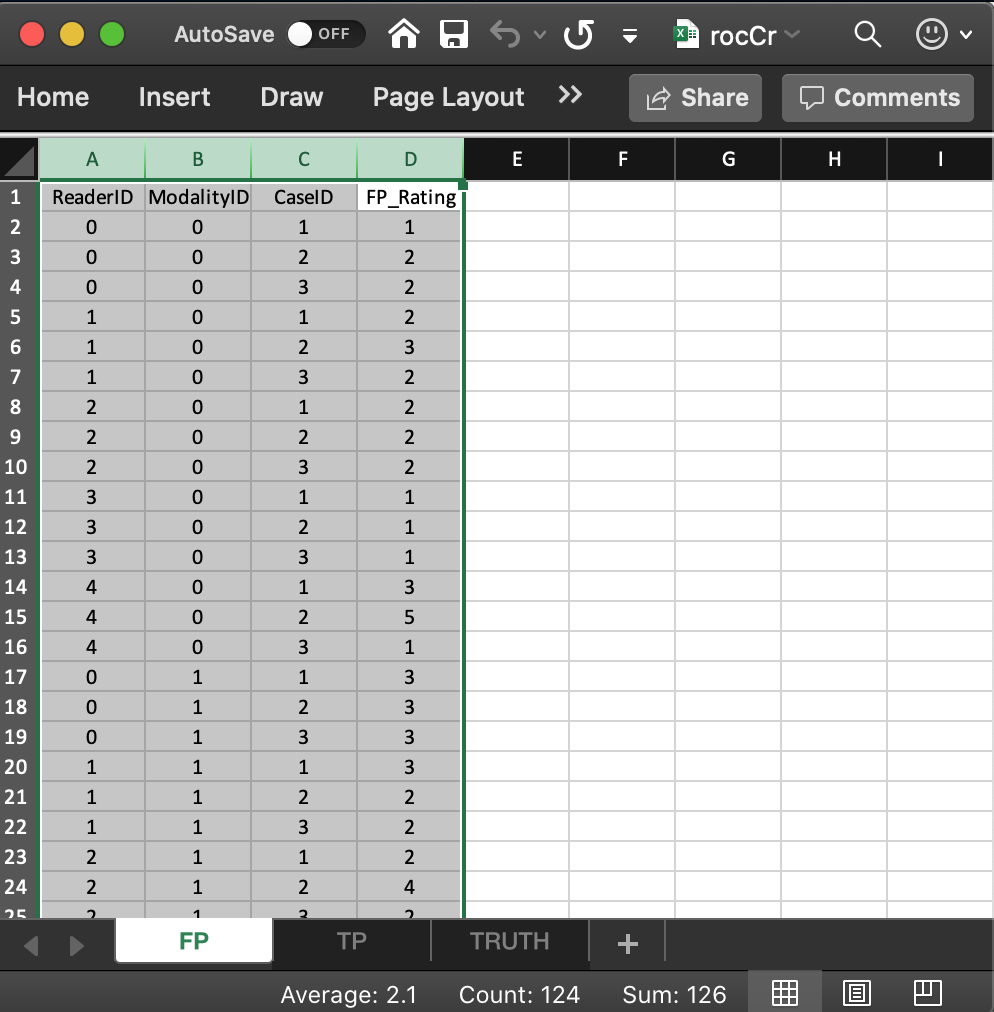
\includegraphics[width=1\textwidth,height=\textheight]{images/quick-start/rocCrFp.png}

\begin{itemize}
\tightlist
\item
  The list member \texttt{x\$ratings\$NL} is an array with \texttt{dim\ =\ c(2,5,8,1)}.

  \begin{itemize}
  \tightlist
  \item
    The first dimension (2) comes from the number of modalities.
  \item
    The second dimension (5) comes from the number of readers.
  \item
    The third dimension (8) comes from the \textbf{total} number of cases.
  \item
    The fourth dimension is always 1 for an ROC dataset.
  \end{itemize}
\item
  The value of \texttt{x\$ratings\$NL{[}1,5,2,1{]}}, i.e., 5, corresponds to row 15 of the FP table, i.e., to \texttt{ModalityID} = 0, \texttt{ReaderID} = 4 and \texttt{CaseID} = 2.
\item
  The value of \texttt{x\$ratings\$NL{[}2,3,2,1{]}}, i.e., 4, corresponds to row 24 of the FP table, i.e., to \texttt{ModalityID} 1, \texttt{ReaderID} 2 and \texttt{CaseID} 2.
\item
  All values for case index \textgreater{} 3 and case index \textless= 8 are \texttt{-Inf}. For example the value of \texttt{x\$ratings\$NL{[}2,3,4,1{]}} is \texttt{-Inf}. This is because there are only 3 non-diseased cases. The extra length is needed for compatibility with FROC datasets.
\end{itemize}

\hypertarget{dataset-object-details-read-datafile-correspondence-ll-tp}{%
\subsection{\texorpdfstring{The \texttt{TP} worksheet}{The TP worksheet}}\label{dataset-object-details-read-datafile-correspondence-ll-tp}}

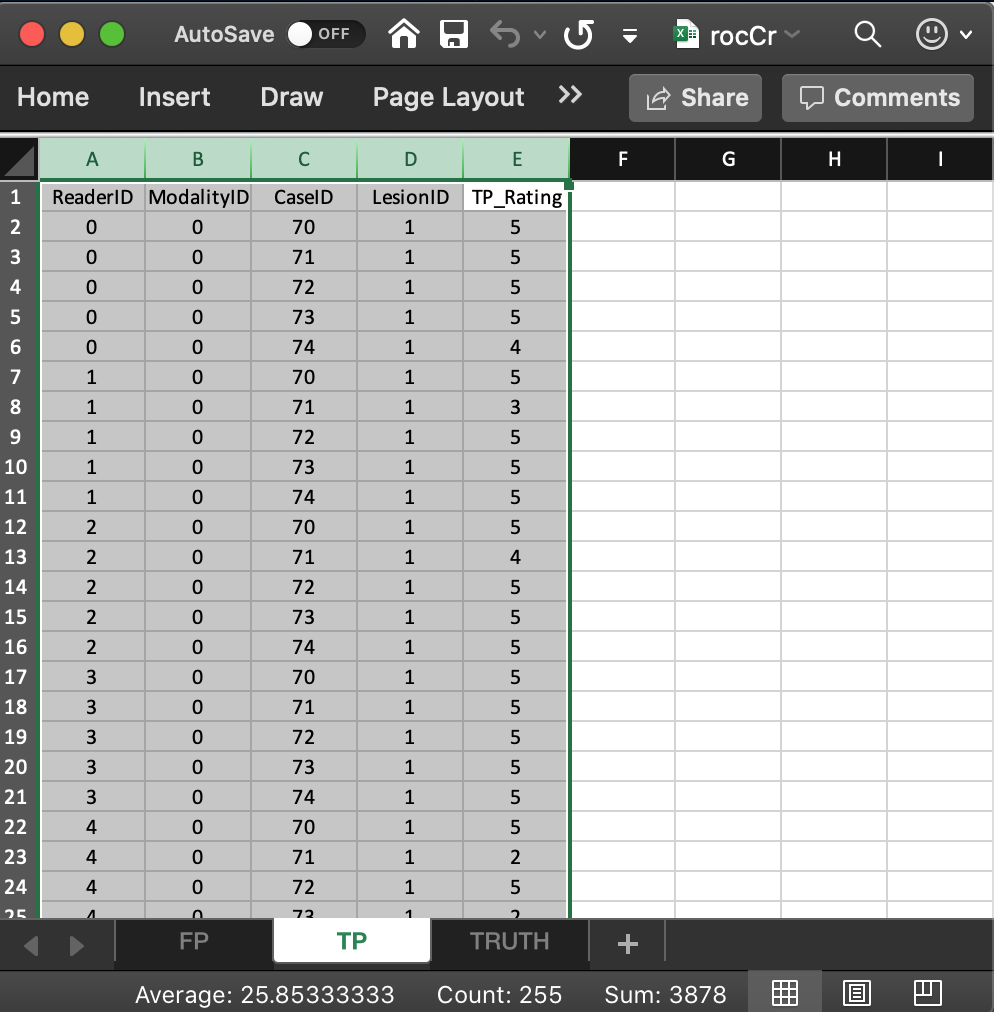
\includegraphics[width=1\textwidth,height=\textheight]{images/quick-start/rocCrTp.png}

\begin{itemize}
\tightlist
\item
  The list member \texttt{x\$ratings\$LL} is an array with \texttt{dim\ =\ c(2,5,5,1)}.

  \begin{itemize}
  \tightlist
  \item
    The first dimension (2) comes from the number of modalities.
  \item
    The second dimension (5) comes from the number of readers.
  \item
    The third dimension (5) comes from the number of diseased cases.
  \item
    The fourth dimension is always 1 for an ROC dataset.
  \end{itemize}
\item
  The value of \texttt{x\$ratings\$LL{[}1,1,5,1{]}}, i.e., 4, corresponds to row 6 of the TP table, i.e., to \texttt{ModalityID} = 0, \texttt{ReaderID} = 0 and \texttt{CaseID} = 74.
\item
  The value of \texttt{x\$ratings\$LL{[}1,2,2,1{]}}, i.e., 3, corresponds to row 8 of the TP table, i.e., to \texttt{ModalityID} = 0, \texttt{ReaderID} = 1 and \texttt{CaseID} = 71.
\item
  The value of \texttt{x\$ratings\$LL{[}1,4,4,1{]}}, i.e., 5, corresponds to row 21 of the TP table, i.e., to \texttt{ModalityID} = 0, \texttt{ReaderID} = 3 and \texttt{CaseID} = 74.
\item
  The value of \texttt{x\$ratings\$LL{[}1,5,2,1{]}}, i.e., 2, corresponds to row 23 of the TP table, i.e., to \texttt{ModalityID} = 0, \texttt{ReaderID} = 4 and \texttt{CaseID} = 71.
\item
  There are no \texttt{-Inf} values in \texttt{x\$ratings\$LL}: \texttt{any(x\$ratings\$LL\ ==\ -Inf)} = FALSE. This is true for any ROC dataset.
\end{itemize}

\hypertarget{dataset-object-details-read-datafile-correspondence-case-index-vs-case-id}{%
\subsection{caseIndex vs.~caseID}\label{dataset-object-details-read-datafile-correspondence-case-index-vs-case-id}}

\begin{itemize}
\tightlist
\item
  The \texttt{caseIndex} is the array index used to access elements in the NL and LL arrays. The case-index is always an integer in the range 1, 2, \ldots, up to the array length. Remember that unlike C++, R indexing starts from 1.
\item
  The \texttt{caseID} is any integer value, including zero, used to uniquely label the cases.
\item
  Regardless of what order they occur in the worksheet, the non-diseased cases are always ordered first. In the current example the case indices are 1, 2 and 3, corresponding to the three non-diseased cases with \texttt{caseIDs} equal to 1, 2 and 3.
\item
  Regardless of what order they occur in the worksheet, in the NL array the diseased cases are always ordered \emph{after} the last non-diseased case. In the current example the case indices in the \texttt{NL} array are 4, 5, 6, 7 and 8, corresponding to the five diseased cases with \texttt{caseIDs} equal to 70, 71, 72, 73, and 74. In the \texttt{LL} array they are indexed 1, 2, 3, 4 and 5. Some examples follow:
\item
  \texttt{x\$ratings\$NL{[}1,3,2,1{]}}, a FP rating, refers to \texttt{ModalityID} 0, \texttt{ReaderID} 2 and \texttt{CaseID} 2 (since the modality and reader IDs start with 0).
\item
  \texttt{x\$ratings\$NL{[}2,5,4,1{]}}, a FP rating, refers to \texttt{ModalityID} 1, \texttt{ReaderID} 4 and \texttt{CaseID} 70, the first diseased case; this is \texttt{-Inf}.
\item
  \texttt{x\$ratings\$NL{[}1,4,8,1{]}}, a FP rating, refers to \texttt{ModalityID} 0, \texttt{ReaderID} 3 and \texttt{CaseID} 74, the last diseased case; this is \texttt{-Inf}.
\item
  \texttt{x\$ratings\$NL{[}1,3,9,1{]}}, a FP rating, is an illegal value, as the third index cannot exceed 8.
\item
  \texttt{x\$ratings\$NL{[}1,3,8,2{]}}, a FP rating, is an illegal value, as the fourth index cannot exceed 1 for an ROC dataset.
\item
  \texttt{x\$ratings\$LL{[}1,3,1,1{]}}, a TP rating, refers to \texttt{ModalityID} 0, \texttt{ReaderID} 2 and \texttt{CaseID} 70, the first diseased case.
\item
  \texttt{x\$ratings\$LL{[}2,5,4,1{]}}, a TP rating, refers to \texttt{ModalityID} 1, \texttt{ReaderID} 4 and \texttt{CaseID} 73, the fourth diseased case.
\end{itemize}

\hypertarget{dataset-object-details-froc-dataset}{%
\section{FROC dataset}\label{dataset-object-details-froc-dataset}}

\includegraphics[width=1\textwidth,height=\textheight]{images/software-details/frocCrTruth.png}

\hypertarget{dataset-object-details-structure-froc-dataset}{%
\subsection{The structure of a factorial FROC dataset}\label{dataset-object-details-structure-froc-dataset}}

\begin{Shaded}
\begin{Highlighting}[]
\NormalTok{x }\OtherTok{\textless{}{-}} \FunctionTok{DfReadDataFile}\NormalTok{(}\StringTok{"images/software{-}details/frocCr.xlsx"}\NormalTok{, }\AttributeTok{newExcelFileFormat =} \ConstantTok{TRUE}\NormalTok{)}
\end{Highlighting}
\end{Shaded}

The dataset \texttt{x} is a \texttt{list} variable with 3 members: \texttt{x\$ratings}, \texttt{x\$lesions} and \texttt{x\$descriptions}.

\begin{Shaded}
\begin{Highlighting}[]
\FunctionTok{str}\NormalTok{(x, }\AttributeTok{max.level =} \DecValTok{1}\NormalTok{)}
\CommentTok{\#\textgreater{} List of 3}
\CommentTok{\#\textgreater{}  $ ratings     :List of 3}
\CommentTok{\#\textgreater{}  $ lesions     :List of 3}
\CommentTok{\#\textgreater{}  $ descriptions:List of 7}
\end{Highlighting}
\end{Shaded}

The \texttt{x\$ratings} member contains 3 sub-lists.

\begin{Shaded}
\begin{Highlighting}[]
\FunctionTok{str}\NormalTok{(x}\SpecialCharTok{$}\NormalTok{ratings)}
\CommentTok{\#\textgreater{} List of 3}
\CommentTok{\#\textgreater{}  $ NL   : num [1:2, 1:3, 1:8, 1:2] 1.02 2.89 2.21 3.01 2.14 ...}
\CommentTok{\#\textgreater{}  $ LL   : num [1:2, 1:3, 1:5, 1:3] 5.28 5.2 5.14 4.77 4.66 4.87 3.01 3.27 3.31 3.19 ...}
\CommentTok{\#\textgreater{}  $ LL\_IL: logi NA}
\end{Highlighting}
\end{Shaded}

\begin{itemize}
\tightlist
\item
  There are \texttt{K2\ =\ 5} diseased cases (the length of the third dimension of \texttt{x\$ratings\$LL}) and \texttt{K1\ =\ 3} non-diseased cases (the length of the third dimension of \texttt{x\$ratings\$NL} minus \texttt{K2}).
\item
  \texttt{x\$ratings\$NL}, a {[}2, 3, 8, 2{]} array, contains the NL ratings on non-diseased and diseased cases.
\item
  \texttt{x\$ratings\$LL}, a {[}2, 3, 5, 3{]} array, contains the ratings of LLs on diseased cases.
\item
  \texttt{x\$ratings\$LL\_IL} is \texttt{NA}, this field applies to an LROC dataset (contains incorrect localizations on diseased cases).
\end{itemize}

The \texttt{x\$lesions} member contains 3 sub-lists.

\begin{Shaded}
\begin{Highlighting}[]
\FunctionTok{str}\NormalTok{(x}\SpecialCharTok{$}\NormalTok{lesions)}
\CommentTok{\#\textgreater{} List of 3}
\CommentTok{\#\textgreater{}  $ perCase: int [1:5] 2 1 3 2 1}
\CommentTok{\#\textgreater{}  $ IDs    : num [1:5, 1:3] 1 1 1 1 1 ...}
\CommentTok{\#\textgreater{}  $ weights: num [1:5, 1:3] 0.3 1 0.333 0.1 1 ...}
\end{Highlighting}
\end{Shaded}

\begin{itemize}
\tightlist
\item
  \texttt{x\$lesions\$perCase} is the number of lesions per diseased case vector, i.e., 2, 1, 3, 2, 1.
\item
  \texttt{max(x\$lesions\$perCase)} is the maximum number of lesions per case, i.e., \texttt{r}max(x\(lesions\)perCase)`.
\item
  \texttt{x\$lesions\$weights} is the weights of lesions.
\end{itemize}

\begin{Shaded}
\begin{Highlighting}[]
\NormalTok{x}\SpecialCharTok{$}\NormalTok{lesions}\SpecialCharTok{$}\NormalTok{weights}
\CommentTok{\#\textgreater{}           [,1]      [,2]      [,3]}
\CommentTok{\#\textgreater{} [1,] 0.3000000 0.7000000      {-}Inf}
\CommentTok{\#\textgreater{} [2,] 1.0000000      {-}Inf      {-}Inf}
\CommentTok{\#\textgreater{} [3,] 0.3333333 0.3333333 0.3333333}
\CommentTok{\#\textgreater{} [4,] 0.1000000 0.9000000      {-}Inf}
\CommentTok{\#\textgreater{} [5,] 1.0000000      {-}Inf      {-}Inf}
\end{Highlighting}
\end{Shaded}

The weights for the first diseased case are 0.3 and 0.7. The weight for the second diseased case is 1. For the third diseased case the three weights are 1/3 each, etc. For each diseased case the finite weights sum to unity.

\texttt{x\$descriptions} contains 7 sub-lists.

\begin{Shaded}
\begin{Highlighting}[]
\FunctionTok{str}\NormalTok{(x}\SpecialCharTok{$}\NormalTok{descriptions)}
\CommentTok{\#\textgreater{} List of 7}
\CommentTok{\#\textgreater{}  $ fileName     : chr "frocCr"}
\CommentTok{\#\textgreater{}  $ type         : chr "FROC"}
\CommentTok{\#\textgreater{}  $ name         : logi NA}
\CommentTok{\#\textgreater{}  $ truthTableStr: num [1:2, 1:3, 1:8, 1:4] 1 1 1 1 1 1 1 1 1 1 ...}
\CommentTok{\#\textgreater{}  $ design       : chr "FCTRL"}
\CommentTok{\#\textgreater{}  $ modalityID   : Named chr [1:2] "0" "1"}
\CommentTok{\#\textgreater{}   ..{-} attr(*, "names")= chr [1:2] "0" "1"}
\CommentTok{\#\textgreater{}  $ readerID     : Named chr [1:3] "0" "1" "2"}
\CommentTok{\#\textgreater{}   ..{-} attr(*, "names")= chr [1:3] "0" "1" "2"}
\end{Highlighting}
\end{Shaded}

\begin{itemize}
\tightlist
\item
  \texttt{x\$descriptions\$filename} is for internal use.
\item
  \texttt{x\$descriptions\$type} is FROC, which specifies the data collection method.
\item
  \texttt{x\$descriptions\$name} is for internal use.
\item
  \texttt{x\$descriptions\$truthTableStr} is for internal use; it quantifies the structure of the dataset; it is explained in the next section.
\item
  \texttt{x\$descriptions\$design} is FCTRL; it specifies the study design.
\item
  \texttt{x\$descriptions\$modalityID} is a vector with two elements 0, 1 naming the two modalities.
\item
  \texttt{x\$readerID} is a vector with three elements 0, 1, 2 naming the three readers.
\end{itemize}

\hypertarget{dataset-object-truth-table-str}{%
\subsection{\texorpdfstring{\texttt{truthTableStr}}{truthTableStr}}\label{dataset-object-truth-table-str}}

\begin{itemize}
\tightlist
\item
  For this dataset \texttt{I} = 2, \texttt{J} = 3 and \texttt{K} = 8.
\item
  \texttt{truthTableStr} is a \texttt{2\ x\ 3\ x\ 8\ x\ 4} array, i.e., \texttt{I} x \texttt{J} x \texttt{K} x (maximum number of lesions per case plus 1 - the \texttt{plus\ 1} is needed to accommodate non-diseased cases).
\item
  Each entry in this array is either \texttt{1}, meaning the corresponding interpretation happened, or \texttt{NA}, meaning the corresponding interpretation did not happen.
\end{itemize}

\hypertarget{explanation-for-non-diseased-cases}{%
\subsubsection{Explanation for non-diseased cases}\label{explanation-for-non-diseased-cases}}

Since the fourth index is set to 1, in the following code only non-diseased cases yield ones and all diseased cases yield \texttt{NA}.

\begin{Shaded}
\begin{Highlighting}[]
\FunctionTok{all}\NormalTok{(x}\SpecialCharTok{$}\NormalTok{descriptions}\SpecialCharTok{$}\NormalTok{truthTableStr[,,}\DecValTok{1}\SpecialCharTok{:}\DecValTok{3}\NormalTok{,}\DecValTok{1}\NormalTok{] }\SpecialCharTok{==}\DecValTok{1}\NormalTok{)}
\CommentTok{\#\textgreater{} [1] TRUE}
\FunctionTok{all}\NormalTok{(}\FunctionTok{is.na}\NormalTok{(x}\SpecialCharTok{$}\NormalTok{descriptions}\SpecialCharTok{$}\NormalTok{truthTableStr[,,}\DecValTok{4}\SpecialCharTok{:}\DecValTok{8}\NormalTok{,}\DecValTok{1}\NormalTok{]))}
\CommentTok{\#\textgreater{} [1] TRUE}
\end{Highlighting}
\end{Shaded}

\hypertarget{explanation-for-diseased-cases-with-one-lesion}{%
\subsubsection{Explanation for diseased cases with one lesion}\label{explanation-for-diseased-cases-with-one-lesion}}

Since the fourth index is set to 2, in the following code all non-diseased cases yield \texttt{NA} and all diseased cases yield 1 as all diseased cases have at least one lesion.

\begin{Shaded}
\begin{Highlighting}[]
\FunctionTok{all}\NormalTok{(}\FunctionTok{is.na}\NormalTok{(x}\SpecialCharTok{$}\NormalTok{descriptions}\SpecialCharTok{$}\NormalTok{truthTableStr[,,}\DecValTok{1}\SpecialCharTok{:}\DecValTok{3}\NormalTok{,}\DecValTok{2}\NormalTok{]))}
\CommentTok{\#\textgreater{} [1] TRUE}
\FunctionTok{all}\NormalTok{(x}\SpecialCharTok{$}\NormalTok{descriptions}\SpecialCharTok{$}\NormalTok{truthTableStr[,,}\DecValTok{4}\SpecialCharTok{:}\DecValTok{8}\NormalTok{,}\DecValTok{2}\NormalTok{] }\SpecialCharTok{==} \DecValTok{1}\NormalTok{)}
\CommentTok{\#\textgreater{} [1] TRUE}
\end{Highlighting}
\end{Shaded}

\hypertarget{explanation-for-diseased-cases-with-two-lesions}{%
\subsubsection{Explanation for diseased cases with two lesions}\label{explanation-for-diseased-cases-with-two-lesions}}

Since the fourth index is set to 3, in the following code all non-diseased cases yield \texttt{NA}; the first diseased case \texttt{70} yields 1 (this case contains two lesions); the second disease case \texttt{71} yields \texttt{NA} (this case contains only one lesion); the third disease case \texttt{72} yields \texttt{NA} (this case contains only two lesions); the fourth disease case \texttt{73} yields 1 (this case contains two lesions); the fifth disease case \texttt{74} yields \texttt{NA} (this case contains one lesion).

\begin{Shaded}
\begin{Highlighting}[]
\CommentTok{\# all non diseased cases}
\FunctionTok{all}\NormalTok{(}\FunctionTok{is.na}\NormalTok{(x}\SpecialCharTok{$}\NormalTok{descriptions}\SpecialCharTok{$}\NormalTok{truthTableStr[,,}\DecValTok{1}\SpecialCharTok{:}\DecValTok{3}\NormalTok{,}\DecValTok{3}\NormalTok{]))}
\CommentTok{\#\textgreater{} [1] TRUE}
\CommentTok{\# first diseased case}
\FunctionTok{all}\NormalTok{(x}\SpecialCharTok{$}\NormalTok{descriptions}\SpecialCharTok{$}\NormalTok{truthTableStr[,,}\DecValTok{4}\NormalTok{,}\DecValTok{3}\NormalTok{] }\SpecialCharTok{==} \DecValTok{1}\NormalTok{)}
\CommentTok{\#\textgreater{} [1] TRUE}
\CommentTok{\# second diseased case}
\FunctionTok{all}\NormalTok{(}\FunctionTok{is.na}\NormalTok{(x}\SpecialCharTok{$}\NormalTok{descriptions}\SpecialCharTok{$}\NormalTok{truthTableStr[,,}\DecValTok{5}\NormalTok{,}\DecValTok{3}\NormalTok{]))}
\CommentTok{\#\textgreater{} [1] TRUE}
\CommentTok{\# third diseased case}
\FunctionTok{all}\NormalTok{(x}\SpecialCharTok{$}\NormalTok{descriptions}\SpecialCharTok{$}\NormalTok{truthTableStr[,,}\DecValTok{6}\NormalTok{,}\DecValTok{3}\NormalTok{] }\SpecialCharTok{==} \DecValTok{1}\NormalTok{)}
\CommentTok{\#\textgreater{} [1] TRUE}
\CommentTok{\# fourth diseased case}
\FunctionTok{all}\NormalTok{(x}\SpecialCharTok{$}\NormalTok{descriptions}\SpecialCharTok{$}\NormalTok{truthTableStr[,,}\DecValTok{7}\NormalTok{,}\DecValTok{3}\NormalTok{] }\SpecialCharTok{==} \DecValTok{1}\NormalTok{)}
\CommentTok{\#\textgreater{} [1] TRUE}
\CommentTok{\# fifth diseased case}
\FunctionTok{all}\NormalTok{(}\FunctionTok{is.na}\NormalTok{(x}\SpecialCharTok{$}\NormalTok{descriptions}\SpecialCharTok{$}\NormalTok{truthTableStr[,,}\DecValTok{8}\NormalTok{,}\DecValTok{3}\NormalTok{]))}
\CommentTok{\#\textgreater{} [1] TRUE}
\end{Highlighting}
\end{Shaded}

\hypertarget{explanation-for-diseased-cases-with-three-lesions}{%
\subsubsection{Explanation for diseased cases with three lesions}\label{explanation-for-diseased-cases-with-three-lesions}}

Since the fourth index is set to 4, in the following code all non-diseased cases yield \texttt{NA}; the first diseased case \texttt{70} yields \texttt{NA} (this case contains two lesions); the second disease case \texttt{71} yields \texttt{NA} (this case contains one lesion); the third disease case \texttt{72} yields \texttt{NA} (this case contains two lesions); the fourth disease case \texttt{73} yields 1 (this case contains three lesions); the fifth disease case \texttt{74} yields \texttt{NA} (this case contains one lesion).

\begin{Shaded}
\begin{Highlighting}[]
\CommentTok{\# all non diseased cases}
\FunctionTok{all}\NormalTok{(}\FunctionTok{is.na}\NormalTok{(x}\SpecialCharTok{$}\NormalTok{descriptions}\SpecialCharTok{$}\NormalTok{truthTableStr[,,}\DecValTok{1}\SpecialCharTok{:}\DecValTok{3}\NormalTok{,}\DecValTok{4}\NormalTok{]))}
\CommentTok{\#\textgreater{} [1] TRUE}
\CommentTok{\# first diseased case}
\FunctionTok{all}\NormalTok{(}\FunctionTok{is.na}\NormalTok{(x}\SpecialCharTok{$}\NormalTok{descriptions}\SpecialCharTok{$}\NormalTok{truthTableStr[,,}\DecValTok{4}\NormalTok{,}\DecValTok{4}\NormalTok{]))}
\CommentTok{\#\textgreater{} [1] TRUE}
\CommentTok{\# second diseased case}
\FunctionTok{all}\NormalTok{(}\FunctionTok{is.na}\NormalTok{(x}\SpecialCharTok{$}\NormalTok{descriptions}\SpecialCharTok{$}\NormalTok{truthTableStr[,,}\DecValTok{5}\NormalTok{,}\DecValTok{4}\NormalTok{]))}
\CommentTok{\#\textgreater{} [1] TRUE}
\CommentTok{\# third diseased case}
\FunctionTok{all}\NormalTok{(x}\SpecialCharTok{$}\NormalTok{descriptions}\SpecialCharTok{$}\NormalTok{truthTableStr[,,}\DecValTok{6}\NormalTok{,}\DecValTok{4}\NormalTok{] }\SpecialCharTok{==} \DecValTok{1}\NormalTok{)}
\CommentTok{\#\textgreater{} [1] TRUE}
\CommentTok{\# fourth diseased case}
\FunctionTok{all}\NormalTok{(}\FunctionTok{is.na}\NormalTok{(x}\SpecialCharTok{$}\NormalTok{descriptions}\SpecialCharTok{$}\NormalTok{truthTableStr[,,}\DecValTok{7}\NormalTok{,}\DecValTok{4}\NormalTok{]))}
\CommentTok{\#\textgreater{} [1] TRUE}
\CommentTok{\# fifth diseased case}
\FunctionTok{all}\NormalTok{(}\FunctionTok{is.na}\NormalTok{(x}\SpecialCharTok{$}\NormalTok{descriptions}\SpecialCharTok{$}\NormalTok{truthTableStr[,,}\DecValTok{8}\NormalTok{,}\DecValTok{4}\NormalTok{]))}
\CommentTok{\#\textgreater{} [1] TRUE}
\end{Highlighting}
\end{Shaded}

\hypertarget{the-fp-worksheet}{%
\subsection{The FP worksheet}\label{the-fp-worksheet}}

These are found in the \texttt{FP} or \texttt{NL} worksheet:

\includegraphics[width=1\textwidth,height=\textheight]{images/software-details/frocCrFp.png}

\begin{itemize}
\tightlist
\item
  The common vertical length is 22 in this example.
\item
  \texttt{ReaderID}: the reader labels: \texttt{0}, 1\texttt{,}2\texttt{,\ as\ declared\ in\ the}Truth` worksheet.
\item
  \texttt{ModalityID}: the modality labels: \texttt{0} or \texttt{1}, as declared in the \texttt{Truth} worksheet.
\item
  \texttt{CaseID}: \texttt{1}, \texttt{2}, \texttt{3}, \texttt{71}, \texttt{72}, \texttt{73}, \texttt{74}, as declared in the \texttt{Truth} worksheet; note that not all cases have NL marks on them.\\
\item
  \texttt{NL\_Rating}: the ratings of non-diseased cases.
\end{itemize}

\hypertarget{the-tp-worksheet}{%
\subsection{The TP worksheet}\label{the-tp-worksheet}}

These are found in the \texttt{TP} or \texttt{LL} worksheet, see below.

\includegraphics[width=1\textwidth,height=\textheight]{images/software-details/frocCrTp.png}

\begin{itemize}
\tightlist
\item
  This worksheet has the ratings of diseased cases.
\item
  \texttt{ReaderID}: the reader labels: these must be from \texttt{0}, \texttt{1}, \texttt{2}, as declared in the \texttt{Truth} worksheet.
\item
  \texttt{ModalityID}: \texttt{0} or \texttt{1}, as declared in the \texttt{Truth} worksheet.
\item
  \texttt{CaseID}: these must be from \texttt{70}, \texttt{71}, \texttt{72}, \texttt{73}, \texttt{74}, as declared in the \texttt{Truth} worksheet; not all diseased cases have LL marks.\\
\item
  \texttt{LL\_Rating}: the ratings of diseased cases.
\end{itemize}

\hypertarget{part-datasets}{%
\part*{DATASETS}\label{part-datasets}}
\addcontentsline{toc}{part}{DATASETS}

\hypertarget{datasets}{%
\chapter{Datasets}\label{datasets}}

\hypertarget{datasets-datasetsdd}{%
\section{\texorpdfstring{Datasets embedded in \texttt{RJafroc}}{Datasets embedded in RJafroc}}\label{datasets-datasetsdd}}

They are identified in the code by dataset\texttt{dd} (where \texttt{dd} is an integer in the range \texttt{01} to \texttt{14}). As an example, \texttt{dataset01} can be viewed \href{https://dpc10ster.github.io/RJafroc/reference/dataset01.html}{here}.

\hypertarget{datasets-dataset01}{%
\subsection{Dataset01}\label{datasets-dataset01}}

\texttt{dataset01} ``TONY'' FROC dataset \citep{chakraborty2011estimating}

\begin{verbatim}
## List of 3
##  $ NL   : num [1:2, 1:5, 1:185, 1:3] 3 -Inf 3 -Inf 4 ...
##  $ LL   : num [1:2, 1:5, 1:89, 1:2] 4 4 3 -Inf 3.5 ...
##  $ LL_IL: logi NA
\end{verbatim}

\hypertarget{datasets-dataset02}{%
\subsection{Dataset02}\label{datasets-dataset02}}

\texttt{dataset02} ``VAN-DYKE'' (Van Dyke) ROC dataset \citep{RN1993}

\begin{verbatim}
## List of 3
##  $ NL   : num [1:2, 1:5, 1:114, 1] 1 3 2 3 2 2 1 2 3 2 ...
##  $ LL   : num [1:2, 1:5, 1:45, 1] 5 5 5 5 5 5 5 5 5 5 ...
##  $ LL_IL: logi NA
\end{verbatim}

\hypertarget{datasets-dataset03}{%
\subsection{Dataset03}\label{datasets-dataset03}}

\texttt{dataset03} ``FRANKEN'' (Franken) ROC dataset \citep{RN1995}

\begin{verbatim}
## List of 3
##  $ NL   : num [1:2, 1:4, 1:100, 1] 3 3 4 3 3 3 4 1 1 3 ...
##  $ LL   : num [1:2, 1:4, 1:67, 1] 5 5 4 4 5 4 4 5 2 2 ...
##  $ LL_IL: logi NA
\end{verbatim}

\hypertarget{datasets-dataset04}{%
\subsection{Dataset04}\label{datasets-dataset04}}

\texttt{dataset04} ``FEDERICA'' (Federica Zanca) FROC dataset \citep{zanca2009evaluation}

\begin{verbatim}
## List of 3
##  $ NL   : num [1:5, 1:4, 1:200, 1:7] -Inf -Inf 1 -Inf -Inf ...
##  $ LL   : num [1:5, 1:4, 1:100, 1:3] 4 5 4 5 4 3 5 4 4 3 ...
##  $ LL_IL: logi NA
\end{verbatim}

\hypertarget{datasets-dataset05}{%
\subsection{Dataset05}\label{datasets-dataset05}}

\texttt{dataset05} ``THOMPSON'' (John Thompson) FROC dataset \citep{RN2368}

\begin{verbatim}
## List of 3
##  $ NL   : num [1:2, 1:9, 1:92, 1:7] 4 5 -Inf -Inf 8 ...
##  $ LL   : num [1:2, 1:9, 1:47, 1:3] 5 9 -Inf 10 8 ...
##  $ LL_IL: logi NA
\end{verbatim}

\hypertarget{datasets-dataset06}{%
\subsection{Dataset06}\label{datasets-dataset06}}

\begin{itemize}
\tightlist
\item
  \texttt{dataset06} ``MAGNUS'' (Magnus Bath) FROC dataset \citep{RN1929}
\end{itemize}

\begin{verbatim}
## List of 3
##  $ NL   : num [1:2, 1:4, 1:89, 1:17] 1 -Inf -Inf -Inf 1 ...
##  $ LL   : num [1:2, 1:4, 1:42, 1:15] -Inf -Inf -Inf -Inf -Inf ...
##  $ LL_IL: logi NA
\end{verbatim}

\hypertarget{datasets-dataset07}{%
\subsection{Dataset07}\label{datasets-dataset07}}

\texttt{dataset07} ``LUCY-WARREN'' (Lucy Warren) FROC dataset \citep{RN2507}

\begin{verbatim}
## List of 3
##  $ NL   : num [1:5, 1:7, 1:162, 1:4] 1 2 1 2 -Inf ...
##  $ LL   : num [1:5, 1:7, 1:81, 1:3] 2 -Inf 2 -Inf 1 ...
##  $ LL_IL: logi NA
\end{verbatim}

\hypertarget{datasets-dataset08}{%
\subsection{Dataset08}\label{datasets-dataset08}}

\texttt{dataset08} ``PENEDO'' (Monica Penedo) FROC dataset \citep{RN1520}

\begin{verbatim}
## List of 3
##  $ NL   : num [1:5, 1:5, 1:112, 1] 3 2 3 2 3 0 0 4 0 2 ...
##  $ LL   : num [1:5, 1:5, 1:64, 1] 3 2 4 3 3 3 3 4 4 3 ...
##  $ LL_IL: logi NA
\end{verbatim}

\hypertarget{datasets-dataset09}{%
\subsection{Dataset09}\label{datasets-dataset09}}

\texttt{dataset09} ``NICO-CAD-ROC'' (Nico Karssemeijer) ROC dataset \citep{hupse2013standalone}

\begin{verbatim}
## List of 3
##  $ NL   : num [1, 1:10, 1:200, 1] 28 0 14 0 16 0 31 0 0 0 ...
##  $ LL   : num [1, 1:10, 1:80, 1] 29 12 13 10 41 67 61 51 67 0 ...
##  $ LL_IL: logi NA
\end{verbatim}

\hypertarget{datasets-dataset10}{%
\subsection{Dataset10}\label{datasets-dataset10}}

\texttt{dataset10} ``RUSCHIN'' (Mark Ruschin) ROC dataset \citep{RN1646}

\begin{verbatim}
## List of 3
##  $ NL   : num [1:3, 1:8, 1:90, 1] 1 0 0 0 0 0 1 0 0 0 ...
##  $ LL   : num [1:3, 1:8, 1:40, 1] 2 1 1 2 0 0 0 0 0 3 ...
##  $ LL_IL: logi NA
\end{verbatim}

\hypertarget{datasets-dataset11}{%
\subsection{Dataset11}\label{datasets-dataset11}}

\texttt{dataset11} ``DOBBINS-1'' (James Dobbins) FROC dataset \citep{Dobbins2016MultiInstitutional}

\begin{verbatim}
## List of 3
##  $ NL   : num [1:4, 1:5, 1:158, 1:4] -Inf -Inf -Inf -Inf -Inf ...
##  $ LL   : num [1:4, 1:5, 1:115, 1:20] -Inf -Inf -Inf -Inf -Inf ...
##  $ LL_IL: logi NA
\end{verbatim}

\hypertarget{datasets-dataset12}{%
\subsection{Dataset12}\label{datasets-dataset12}}

\texttt{dataset12} ``DOBBINS-2'' (James Dobbins) ROC dataset \citep{Dobbins2016MultiInstitutional}

\begin{verbatim}
## List of 3
##  $ NL   : num [1:4, 1:5, 1:152, 1] -Inf -Inf -Inf -Inf -Inf ...
##  $ LL   : num [1:4, 1:5, 1:88, 1] 3 4 4 -Inf -Inf ...
##  $ LL_IL: logi NA
\end{verbatim}

\hypertarget{datasets-dataset13}{%
\subsection{Dataset13}\label{datasets-dataset13}}

\texttt{dataset13} ``DOBBINS-3'' (James Dobbins) FROC dataset \citep{Dobbins2016MultiInstitutional}

\begin{verbatim}
## List of 3
##  $ NL   : num [1:4, 1:5, 1:158, 1:4] -Inf 3 -Inf 4 5 ...
##  $ LL   : num [1:4, 1:5, 1:106, 1:15] -Inf -Inf -Inf -Inf -Inf ...
##  $ LL_IL: logi NA
\end{verbatim}

\hypertarget{datasets-dataset14}{%
\subsection{Dataset14}\label{datasets-dataset14}}

\texttt{dataset14} ``FEDERICA-REAL-ROC'' (Federica Zanca) \emph{real} ROC dataset \citep{zanca2012correlation}

\begin{verbatim}
## List of 3
##  $ NL   : num [1:2, 1:4, 1:200, 1] 2 2 2 2 1 3 2 2 3 1 ...
##  $ LL   : num [1:2, 1:4, 1:100, 1] 6 5 6 4 5 5 5 5 5 4 ...
##  $ LL_IL: logi NA
\end{verbatim}

\hypertarget{other-datasets}{%
\section{Other datasets}\label{other-datasets}}

\hypertarget{datasets-datasetCadLroc}{%
\subsection{DatasetCadLroc}\label{datasets-datasetCadLroc}}

\texttt{datasetCadLroc} ``NICO-CAD-LROC'' (Nico Karssemeijer) standalone CAD LROC dataset

\begin{verbatim}
## List of 3
##  $ NL   : num [1, 1:10, 1:200, 1] 28 0 14 0 16 0 31 0 0 0 ...
##  $ LL   : num [1, 1:10, 1:80, 1] 0 0 0 0 0 0 0 0 67 0 ...
##  $ LL_IL: num [1, 1:10, 1:80, 1] 29 12 13 10 41 67 61 51 0 0 ...
\end{verbatim}

\hypertarget{datasets-datasetCadSimuFroc}{%
\subsection{datasetCadSimuFroc}\label{datasets-datasetCadSimuFroc}}

\texttt{datasetCadSimuFroc} ``SIM-CAD-FROC'' (Nico Karssemeijer) simulated standalone CAD FROC dataset

\begin{verbatim}
## List of 3
##  $ NL   : num [1, 1:10, 1:200, 1] 28 -Inf 14 -Inf 16 ...
##  $ LL   : num [1, 1:10, 1:80, 1] -Inf -Inf -Inf -Inf -Inf ...
##  $ LL_IL: logi NA
\end{verbatim}

  \bibliography{packages.bib,myRefs.bib}

\end{document}
